\documentclass[12pt]{article}
\usepackage[utf8]{inputenc}
%\usepackage[english]{babel}
\usepackage{graphicx,animate}
\usepackage{fancybox,fancyhdr}
\usepackage[pagebackref=true]{hyperref}
\usepackage{placeins}
\usepackage{scalerel}
\usepackage[dvipsnames]{xcolor}
\usepackage{setspace}
\usepackage{mathtools}
\usepackage{wrapfig}
\usepackage{enumitem}
\usepackage{amsmath,amssymb}
\usepackage{indentfirst}
\usepackage{anyfontsize}
\usepackage{listings}
\usepackage{float} % j'ai add ca pour forcer l'image à s'afficher à un endroit précis
\usepackage{graphicx}
\usepackage{subcaption}  % et PAS subfigure (qui est obsolète)

\usepackage[top=2.5cm, bottom=2.5cm,left=1.5cm, right=1.5cm]{geometry}

\usepackage{fancyhdr}
\pagestyle{fancy}

\hypersetup{
    colorlinks=true,
    urlcolor=blue,
    linkcolor=teal,
    citecolor=red,
    breaklinks=true
}

\renewcommand{\headrulewidth}{1pt}
%\fancyhead[C]{\textbf{page \thepage}} 
%\fancyhead[L]{\leftmark}
%\fancyhead[R]{Meet In The Middle}

\renewcommand{\footrulewidth}{1pt}
%\fancyfoot[C]{\textbf{page \thepage}} 
%\fancyfoot[L]{\leftmark}
%\fancyfoot[R]{PPAR}

\renewcommand{\contentsname}{Table des Matières}

\definecolor{grisdufond}{rgb}{0.96,0.96,0.96}
\definecolor{mauvedesstrings}{rgb}{0.58,0,0.82}
\lstset{
  aboveskip=3mm,
  belowskip=-2mm,
  backgroundcolor=\color{grisdufond},
  basicstyle=\footnotesize\ttfamily,
  breakatwhitespace=false,
  breaklines=true,
  captionpos=b,
  commentstyle=\itshape\color{red},
  deletekeywords={set}, %marche pas niksamer
  escapeinside={\%*}{*)},
  extendedchars=true,
  framexleftmargin=16pt,
  framextopmargin=3pt,
  framexbottommargin=6pt,
  frame=tb,
  keepspaces=true,
  keywordstyle=\color{blue},
  language=python,
  literate=
  {²}{{\textsuperscript{2}}}1
  {⁴}{{\textsuperscript{4}}}1
  {⁶}{{\textsuperscript{6}}}1
  {⁸}{{\textsuperscript{8}}}1
  {€}{{\euro{}}}1
  {é}{{\'e}}1
  {è}{{\`{e}}}1
  {ê}{{\^{e}}}1
  {ë}{{\¨{e}}}1
  {É}{{\'{E}}}1
  {Ê}{{\^{E}}}1
  {û}{{\^{u}}}1
  {ù}{{\`{u}}}1
  {â}{{\^{a}}}1
  {à}{{\`{a}}}1
  {á}{{\'{a}}}1
  {ã}{{\~{a}}}1
  {À}{{\`{A}}}1
  {Á}{{\'{A}}}1
  {Â}{{\^{A}}}1
  {Ã}{{\~{A}}}1
  {ç}{{\c{c}}}1
  {Ç}{{\c{C}}}1
  {õ}{{\~{o}}}1
  {ó}{{\'{o}}}1
  {ô}{{\^{o}}}1
  {Õ}{{\~{O}}}1
  {Ó}{{\'{O}}}1
  {Ô}{{\^{O}}}1
  {î}{{\^{i}}}1
  {Î}{{\^{I}}}1
  {í}{{\'{i}}}1
  {Í}{{\~{Í}}}1
  {°}{{\textdegree}}1,
  morekeywords={as},
  numbers=left,
  numbersep=10pt,
  numberstyle=\tiny\color{black},
  rulecolor=\color{black},
  showspaces=false,
  showstringspaces=false,
  showtabs=false,
  stepnumber=1,
  stringstyle=\color{mauvedesstrings},
  tabsize=4,
  title=\lstname,
}

\title{Rapport de stage - METIS/Éveha}
\author{Thomas Aubertier}
\date{22 avril - 15 août 2025}

\begin{document}

\maketitle

\begin{abstract}
        
\end{abstract}

\tableofcontents

\newpage
\section{Introduction}

    Ce stage, réalisé au \href{https://sciences.sorbonne-universite.fr/structures-de-recherche/metis}{laboratoire METIS} et en collaboration avec \href{https://www.eveha.fr/}{Éveha International}, s'est déroulé du 22 avril au 15 août 2025. Son objectif était de travailler sur le traîtement de données géophysiques récoltées avec des appareils électromagnétiques.
    
    Selon le descriptif : "\textit{Le stage s'inscrit dans le cadre des activités de recherche et développement du bureau d'études Éveha International, spécialisé dans les études géophysiques en contextes archéologiques variés, du $\ll$ LabCom $\gg$ Geo-Heritage, dédié au sein de l’UMR 5133 Archéorient, à la recherche et au développement de méthodes pour l'étude du patrimoine, et en partenariat avec l'UMR 7619 METIS, dont les activités de recherche portent sur le développement méthodologique en géophysique appliquée principalement à l’analyse des hydrosystèmes et des sols. Il implique sur la base de code existant l'implémentation en langage Python de processus de traitements géophysique spécifiques à la méthode électromagnétique de type Slingram.}"

    Les réalisations et résultats des différentes tâches seront décrites et détaillées dans les setions suivantes. Cela comprend :

    \begin{enumerate}
        \item[$\bullet$] L'ajustement des données selon différents critères (bases, frontières, interpolations, valeurs manquantes...)
        \item[$\bullet$] La multiplicité des méthodes de représentation des données finales (nuage classique, grille)
        \item[$\bullet$] L'automatisation des phases de traitement, lorsque c'est possible. La possibilité de laisser l'utilisateur prendre la main, si la procédure le nécessite.
        \item[$\bullet$] Le stockage de configurations via fichier JSON.
        \item[$\bullet$] L'interface utilisateur via terminal (cmd ou shell python), puis graphique.
        \item[$\bullet$] La rédaction de documentations pour les fonctions.
        \item[$\bullet$] L'intégration à une librairie python, mise en forme des fonctions réalisées au format "module".
        \item[$\bullet$] La création de notebooks (.ipynb) servant d'exemples d'utilisation de fonctions.
        
    \end{enumerate}

\newpage
\section{Traitement CMD}

\subsection{Détection des frontières}\label{2-front}
\subsubsection{Méthode utilisée}
    L'objectif de cette tâche est de corriger les déformations qui peuvent survenir entre deux récoltes de données. Les conditions extérieures, comme la pluie, peuvent changer les propriétés du sol et avoir un effet sur des mesures effectuées avec le même appareil ; et donc par extension biaiser les données. On cherche à ce que les données récoltées sur un même terrain mais à des temps différents puissent être comparables (subir les mêmes déformations) malgré les changements de conditions.

    Pour cela, on veut calculer des paramètres de correction à partir de deux jeux de données (1 et 2) qui serviront à "décaler" les mesures du jeu 2 pour que les points les plus proches spatialement entre 1 et 2 soient de mesure équivalente. En effet, on fera l'hypothèse que deux points proches dans l'espace auront des valeurs de mesures géophysiques proches.

    Afin de minimiser les incertitudes quant à ce redressement, on cherche à trouver les points de 1 et de 2 se trouvant au plus proche de la frontière entre les deux (ceux qui doivent avoir des mesures similaires).

    L'opération doit respecter au mieux les critères suivants :
    \begin{enumerate}
        \item[\textbf{(1)}] La méthode doit pouvoir s'appliquer à tous les jeux de données électromagnétiques.
        \item[\textbf{(2)}] La méthode doit établir un nombre suffisant de points et les plus répartis possibles sur la frontière pour être représentatif.
        \item[\textbf{(3)}] Deux jeux non frontaliers ne doivent pas posséder de frontière.
        \item[\textbf{(4)}] La complexité doit être raisonnable par rapport au nombre de points (si possible linéaire).
    \end{enumerate}

    Pour la suite, on note $E_1$ et $E_2$ les ensembles de points des deux jeux de données, $E_1^f$ et $E_2^f$ ceux des frontières, $p1 = (x1[i], y1[i])$ et $p2 = (x2[j], y2[j])$ les points de $E_1$ et $E_2$ et leur coordonnées, $d = (x1[i]-x2[j])^{2} + (y1[i]-y2[j])^{2}$ leur distance au carré (qu'on cherche à minimiser, $d_{min}$).\\

    \noindent\textbf{\underline{Solutions envisagées}} :
    \begin{enumerate}
        \item[$\bullet$] \textbf{Force brute} : Trouver la distance minimale $d_{min}$ en calculant la distance de tous les couples de points. Si cette solution marche à coup sûr et permet de trouver le minimum global, sa complexité est en $O(n^{2})$ sur des jeux de données pouvant comporter des milliers de lignes (exigeance \textbf{(4)} non respectée). De plus, même si on s'assure de tirer n couples de points distincts étant les n minimums globaux, ils risquent d'être concentrés sur la même région de la frontière et d'être donc assez peu représentatifs (exigeance \textbf{(2)} non respectée).
        \item[$\bullet$] \textbf{Enveloppe convexe} : Il est possible avec une bibliothèque Python (\href{https://docs.scipy.org/doc/scipy/reference/generated/scipy.spatial.ConvexHull.html}{ConvexHull}) d'établir une couverture convexe d'un ensemble de points avec une complexité $O(nlog(n))$ \footnote{\href{https://stackoverflow.com/questions/13524344/complexity-of-the-quickhull-algorithm}{source}, l'algorithme \texttt{scipy} utilise celui décrit dans le poste.}. À partir des côtés du polygone convexe obtenu, on peut déterminer lesquels font partie de $E_1^f$ et $E_2^f$, puis en déduire les points appartenant à cette frontière. Cependant, établir l'appartenance d'un point à une frontière n'est pas toujours trivial et est ambigü, de même que définir ce qu'est une "frontière" d'un nuage de points (une telle structure ne possède pas de côtés). Mais surtout, il n'y a aucune garantie que le prospecteur parcours une zone convexe en premier lieu. Cette approche ne peut donc répondre à tous les cas (exigeance \textbf{(1)} non respectée).
        \item[$\bullet$] \textbf{Enveloppe non convexe} : Cette méthode souffre sensiblement des mêmes défauts que la précédente, avec une complexité normalement linéaire. De plus, je n'ai jamais réussi à obtenir un résultat exploitable.
    \end{enumerate}
    \textbf{\underline{Solution choisie}} : \textbf{Convergence vers un minimum local} : On part de deux points, un dans chaque ensemble (à priori quelconques) et on calcule leur distance $d_{min}$. À chaque itération, on choisit le point suivant dans la liste de $E_1$ et on calcule $d$. Si $d < d_{min}$, alors on le garde et on itère sur $E_2$, sinon on l'ignore et on continue de chercher dans $E_1$. On continue en alternant la recherche sur $E_1$ et $E_2$, tant que tous les points ne sont pas traités. 
    
    À chaque itération, on avance d'un point soit sur $E_1$ soit sur $E_2$. Aucun point n'est parcouru plusieurs fois. Par conséquent, le nombre d'itération de l'algorithme est toujours égal à $|E_1| + |E_2|$. On notant $n$ le nombre total de points des deux jeux, cette méthode permet donc de trouver en $O(n)$ un minimum local du problème tout en restant plutôt facile à mettre en place \label{2_detec_front_out} (\ref{2_detec_front_in}).

    
    %\vspace{10pt}
    %\textcolor{violet}{Julien : je pense qu'il faut justifier les affirmation concernant les différentes complexités (soit en citant la source qui t'as donné l'information soit en décrivant comment tu l'évalues. Il faudrait également harmoniser le snotation (des fois tu utilise le $O(n)$ et équivalent et des fois non}
    %\vspace{10pt}
    
    Il y a néanmoins plusieurs correctifs à apporter pour palier à certains problèmes. Afin 
    d'éviter les doublons lors de plusieurs itérations, on ne prendra que les points non déjà choisi par l'algorithme. De plus, un biais important peut survenir en fonction du point de départ choisi (pour un même point, on retombe toujours dans la même zone). Ces points seront donc tirés au hasard sur les deux ensembles. Enfin, deux ensembles trop éloignés ne peuvent pas partager de frontières. Il faut donc considérer une distance maximale pour considérer ou non la frontière trouvée.

    Si les fichiers de données contiennent des bases, c'est-à-dire des points servant uniquement à l'étalonnage, il faut les retirer au préalable pour ne pas fausser l'écart. En effet, toutes les bases d'une même prospection sont en principe faites au même endroit.
    
    %\vspace{10pt}
    %\textcolor{violet}{Julien : attention, tu n'as pas décrit le jeu de données auquel tu es confronté, du coup le lecteur lambda ne sait pas ce qu'est une base}
    %\vspace{10pt}

    \begin{figure}[ht!]
        \centering
        \begin{subfigure}[b]{0.475\textwidth}
            \centering
            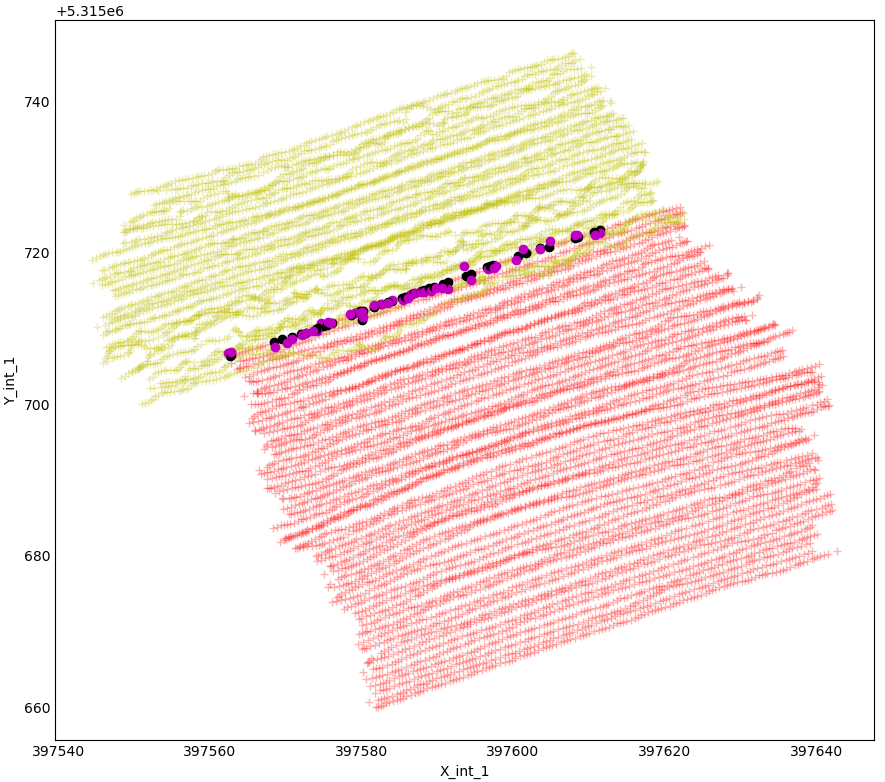
\includegraphics[width=\textwidth]{Images/Frontiere_pts1-3.png}
            \caption[]%
            {{ \small Ensembles avec "superposition".}}    
        \end{subfigure}
        \hfill
        \begin{subfigure}[b]{0.475\textwidth}  
            \centering 
            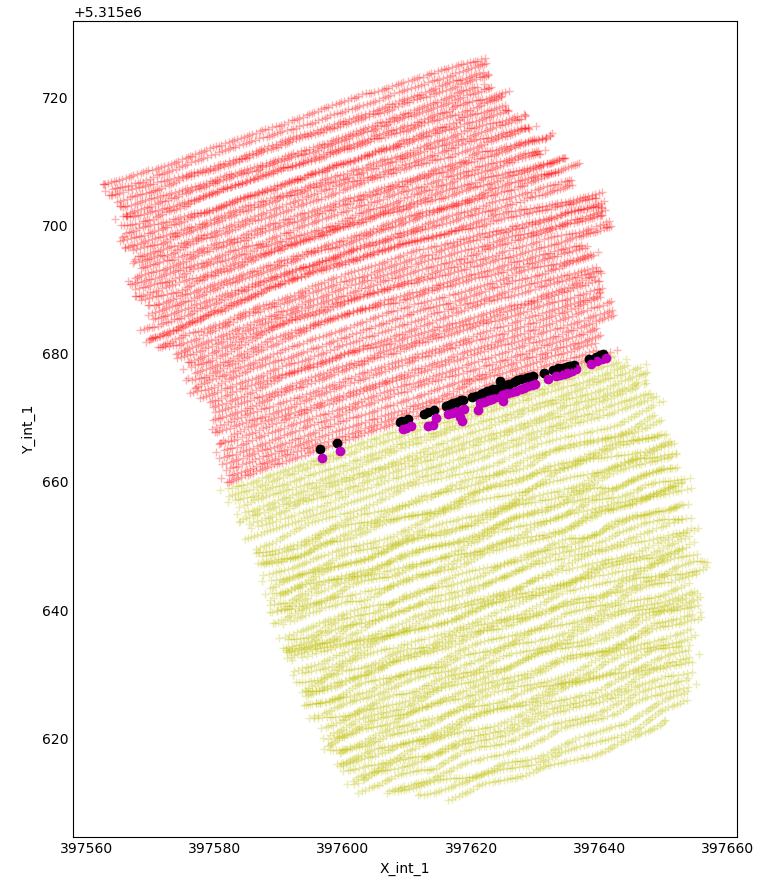
\includegraphics[width=\textwidth]{Images/Frontiere_pts1-2.png}
            \caption[]%
            {{\small Ensembles frontaliers.}}    
        \end{subfigure}
        \caption{25 duos de points sur la frontière, détectés par l'algorithme.}
    \end{figure}
    
    On représente les points choisis en violet et noir. On constate que les distances entre les deux couleurs sont plutôt bien minimisées et se répartissent sur l'ensemble de la frontière.
    
    Selon les hypothèses du modèle, on peut s'attendre à ce que ces points soient suffisament représentatifs de la frontière pour pouvoir effectuer un ajustement efficace par la suite.

    On s'assure de ce que les ensembles non frontaliers ne soient pas détectés comme tels. Par exemple, les deux cas suivants sont exclus :

    \begin{figure}[ht!]
        \centering
        \begin{subfigure}[b]{0.475\textwidth}
            \centering
            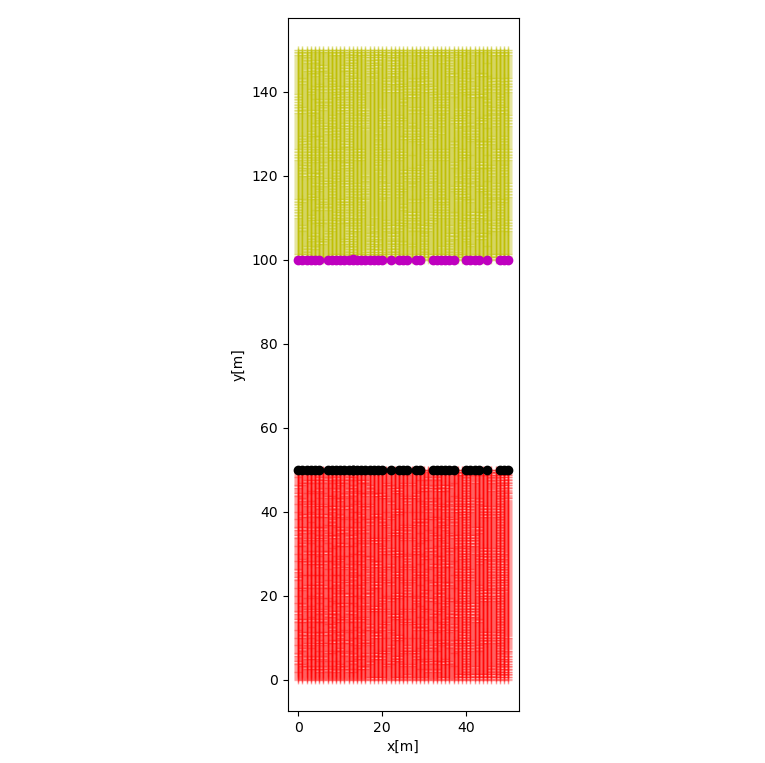
\includegraphics[width=\textwidth]{Images/Frontiere_pts_carre1-5.png}
            \caption[]%
            {{ \small Ensembles trop éloignés.}}    
        \end{subfigure}
        \hfill
        \begin{subfigure}[b]{0.475\textwidth}  
            \centering 
            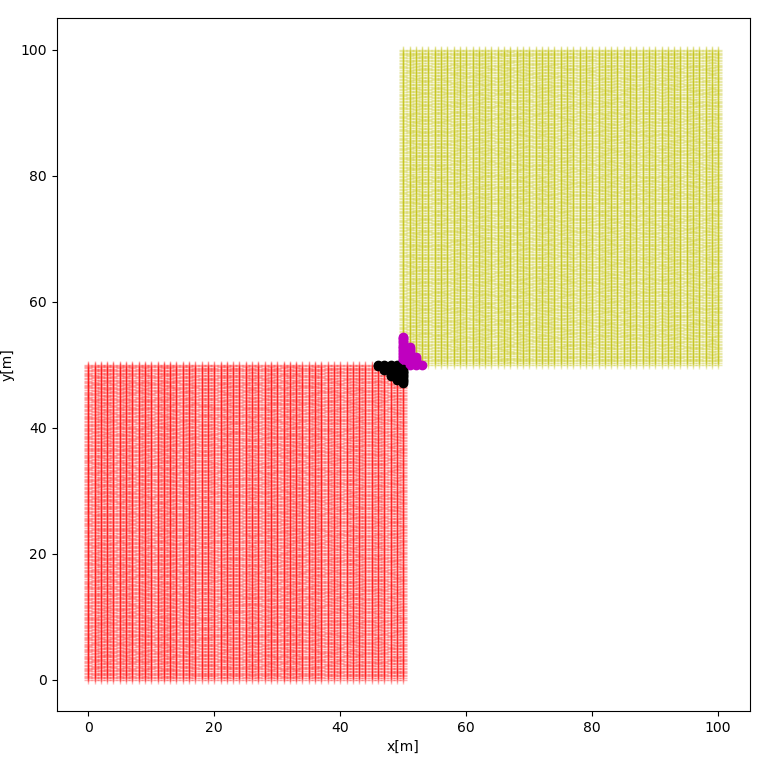
\includegraphics[width=\textwidth]{Images/Frontiere_pts_carre1-3.png}
            \caption[]%
            {{\small Ensembles en contact par un coin.}}    
        \end{subfigure}
        \caption{Cas d'exclusion de frontière.}
    \end{figure}

\subsubsection{Ajustement des données}
    
    On approxime la déformation des données par un modèle linéaire $X = aX' + b$ avec $X'$ la donnée mesuré, $X$ la donnée réelle, $a$ le ratio des écarts types de $E_1^f$ et $E_2^f$ et $b$ la différence de moyenne entre $E_1^f$ et $E_2^f$. On applique cette transformation sur l'ensemble $E_2$.

    \begin{figure}[ht!]
        \begin{center}
            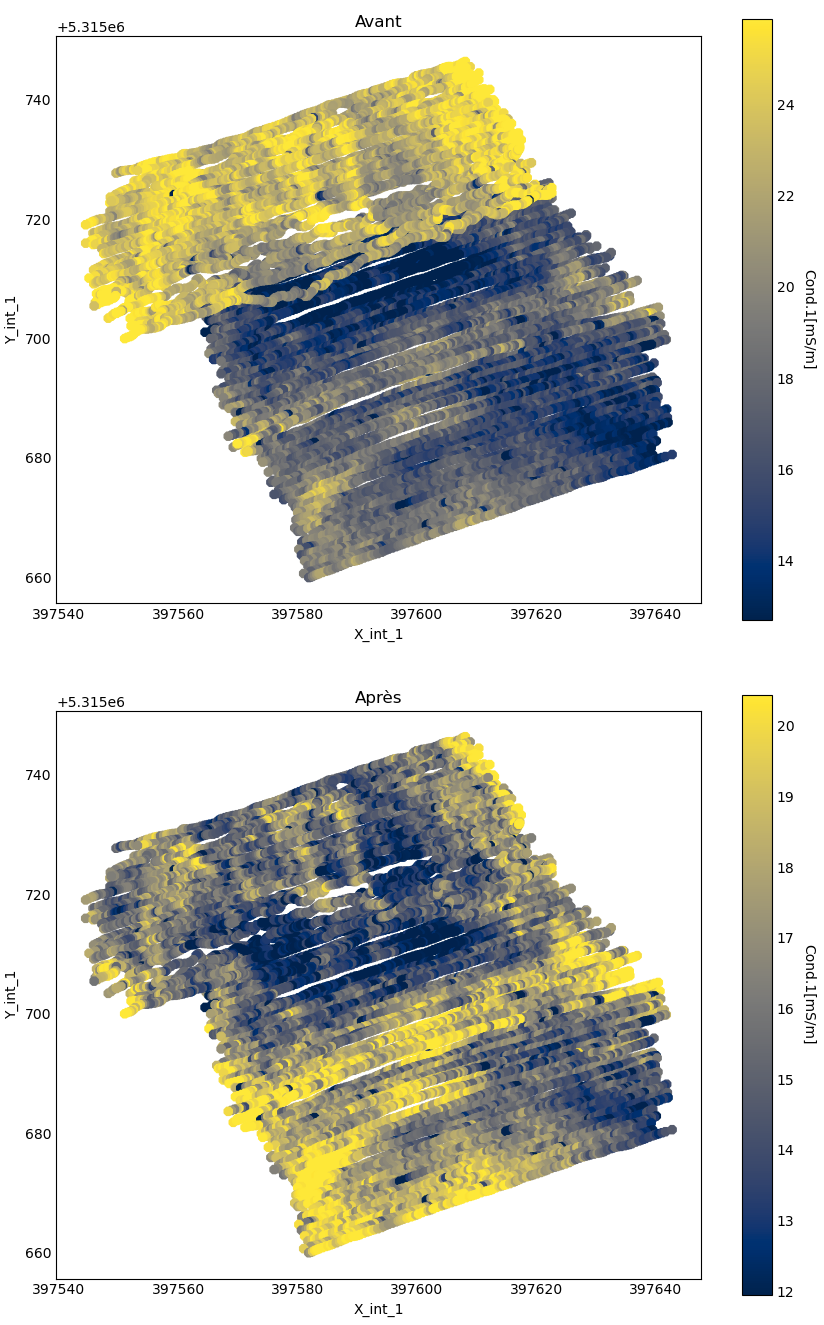
\includegraphics[width=0.72\textwidth]{Images/Frontiere_ajust1-3.png}
            \caption{\label{2_avant_apres}Jeu de données avant et après ajustement.}
        \end{center}
    \end{figure}

    Par exemple, ici (figure \ref{2_avant_apres}), j'ai volontairement bruité le second ensemble par une constante pour renforcer le décalage. On remarque que suite à la rectification, les deux ensembles de départ ne sont plus discernables, ce qui souligne une meilleur cohérence des données.
    
    \label{2_detec_front_ex_out} Un autre exemple est disponible en annexe (\ref{2_detec_front_ex_in}).\\

    Cependant, il peut arriver que l'ajustement proposé dégrade la continuité. En effet, le choix aléatoire et non exhaustif des points couplé à l'erreur intrinsèque du modèle linéaire peut créer un "faux positif" et mal évaluer l'écart entre deux ensemble. Cela peut aussi arriver si un existe un biais fort sur la récolte, comme par exemple si l'appareil est encore en train de démarrer. Si ce cas ne fait pas majorité, on pourrait chercher à le supprimer.
    
    \label{2_detec_front_ex2_out} Pour cette raison, si il le souhaite, l'utilisateur pourra activer un mode plus manuel où il peut valider ou non chaque transformation proposée (pour chaque variable). On peut espérer obtenir un résultat final encore meilleur (\ref{2_detec_front_ex2_in}). En revanche cette étape ne concerne pas les déformations internes à un fichier. Tenter d'évaluer les frontières avant de régler les sauts internes risque de fausser les résultats.

\newpage
\subsubsection{Intérêt de la démarche (frontière)}

    Pour s'assurer de l'intérêt de la méthode comparée à celle consistant à prendre tous les points des ensembles $E_1$ et $E_2$ en considération, prenons un exemple choisi à la main. Les données suivantes ne possèdent pas d'unité à titre d'exemple.

    Soit deux ensembles aléatoires de points sur des espaces rectangulaire, $E_1$ à gauche et $E_2$ à droite. La valeur en chaque point est défini par des lignes de niveaux, de telle sorte que la moyenne des valeurs des points de $E_1$ ($13.67$) soit inférieur à celle de $E_2$ ($26.53$).

    \begin{figure}[ht!]
        \centering
        \begin{subfigure}[b]{0.475\textwidth}
            \centering
            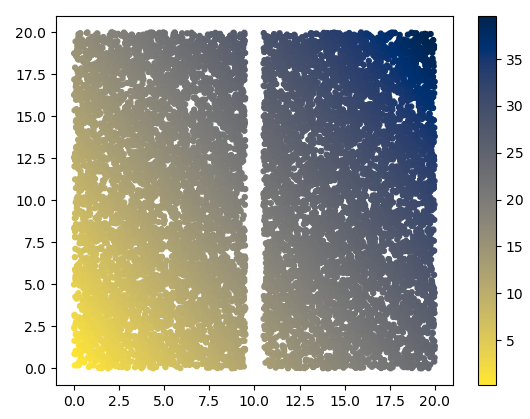
\includegraphics[width=\textwidth]{Images/Frontiere_int_raw.png}
            \caption[]%
            {{ \small Données "réelles" du terrain (bien échelonnées).}}    
        \end{subfigure}
        \hfill
        \begin{subfigure}[b]{0.475\textwidth}  
            \centering 
            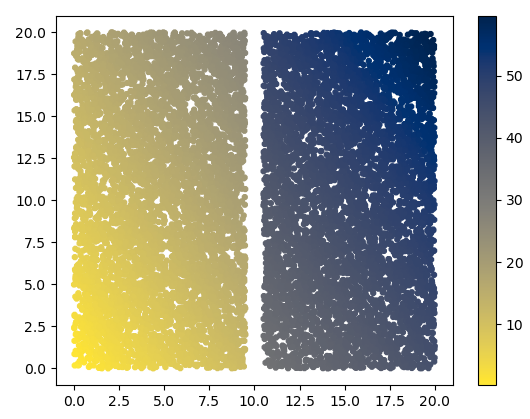
\includegraphics[width=\textwidth]{Images/Frontiere_int_deform.png}
            \caption[]%
            {{\small Données "bruitées" mesurées sur l'ensemble $E_2$.}}    
        \end{subfigure}
        \centering
        \begin{subfigure}[b]{0.475\textwidth}
            \centering
            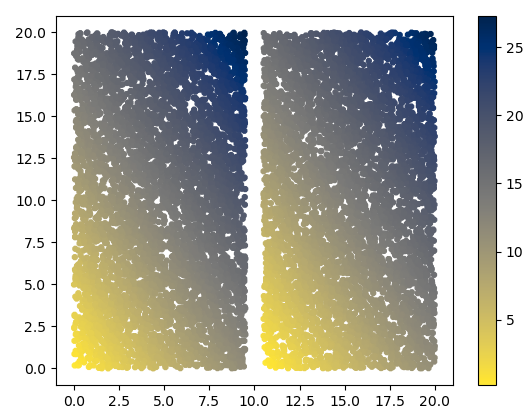
\includegraphics[width=\textwidth]{Images/Frontiere_int_full.png}
            \caption[]%
            {{ \small Échelonnage sur tous les points.}}    
        \end{subfigure}
        \hfill
        \begin{subfigure}[b]{0.475\textwidth}  
            \centering 
            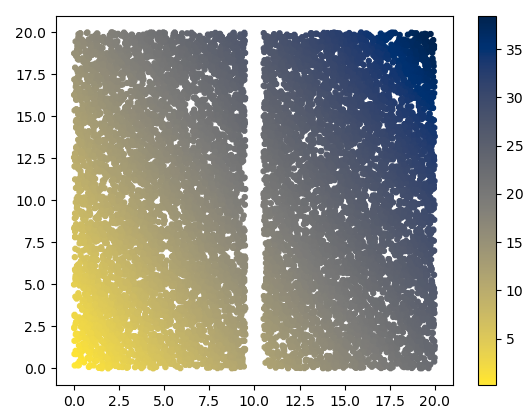
\includegraphics[width=\textwidth]{Images/Frontiere_int_final.png}
            \caption[]%
            {{\small Échelonnage sur la frontière.}}    
        \end{subfigure}
        \caption{Deux techniques de redressement (moyenne différente).}
    \end{figure}

    On suppose que les mesures de l'appareil donnent la figure (b), où on a bruité $E_2$ suivant une loi linéaire. Or on remarque qu'il y a un saut de valeur entre les deux ensembles : la légende indique que l'ensemble $E_2$ possède des valeurs trop élevées par rapport à $E_1$. On voudrait le redresser pour obtenir la figure (a), bien plus cohérente compte tenu des lignes de niveaux des valeurs.

    On applique alors la méthode de redressement décrite précédemment, d'abord en prenant tous les points de l'ensemble (figure (c)) puis seulement ceux trouvés à la frontière (figure (d)).

    Dans le premier cas, on remarque que l'ensemble $E_2$ n'est pas la continuité de l'ensemble $E_1$. Leur moyenne sont identiques (en témoigne les couleurs similaires), mais cela ne regle pas le problème de décalage. En effet, il n'y a aucune raison qu'un découpage d'un ensemble de mesures donne des parcelles de moyenne identiques. La seule hypothèse concernant une quelconque organisation des valeurs est la continuité de la répartition, c'est-à-dire que deux points très proches auront (à forte probabilité) des valeurs mesurées très proches. C'est pour cette raison qu'il est important de d'abord estimer les points frontaliers à l'ensembles, car cela permet de réduire au maximum l'erreur lié à l'évolution du terrain.

    En se concentrant sur les points frontaliers, en l'occurence ceux le plus au centre, on retrouve la continuité de la couleur ; si bien que le résultat est indissociable du jeu initial (a).

\newpage
\subsubsection{Intérêt de la démarche (modèle linéaire)}

    De même manière, on peut refaire la même procédure pour justifier l'utilisation d'une transformation linéaire plutôt que simplement ajouter une constante. Ici l'ensemble $E_2$ subit une déformation réduisant grandement son écart type.

    \begin{figure}[ht!]
        \centering
        \begin{subfigure}[b]{0.475\textwidth}
            \centering
            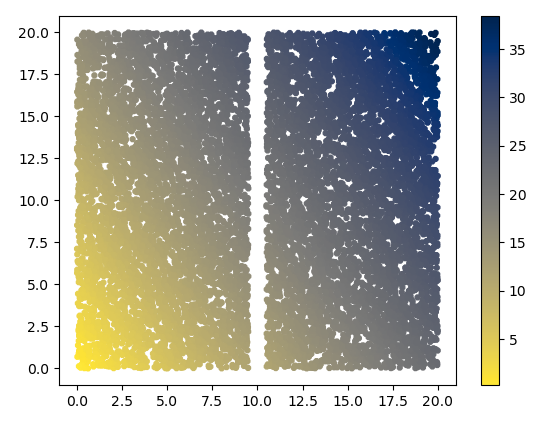
\includegraphics[width=\textwidth]{Images/Frontiere_int2_raw.png}
            \caption[]%
            {{ \small Données "réelles" du terrain (bien échelonnées).}}    
        \end{subfigure}
        \hfill
        \begin{subfigure}[b]{0.475\textwidth}  
            \centering 
            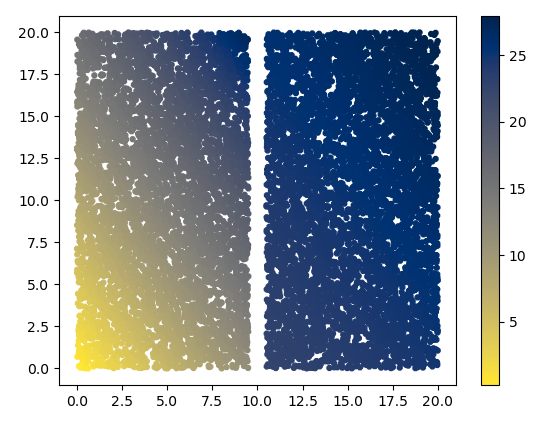
\includegraphics[width=\textwidth]{Images/Frontiere_int2_deform.png}
            \caption[]%
            {{\small Données "bruitées" mesurées sur l'ensemble $E_2$.}}    
        \end{subfigure}
        \centering
        \begin{subfigure}[b]{0.475\textwidth}
            \centering
            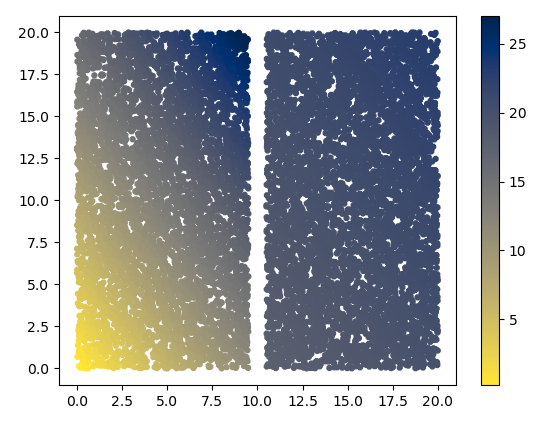
\includegraphics[width=\textwidth]{Images/Frontiere_int2_nostd.png}
            \caption[]%
            {{ \small Échelonnage sans écart type.}}    
        \end{subfigure}
        \hfill
        \begin{subfigure}[b]{0.475\textwidth}  
            \centering 
            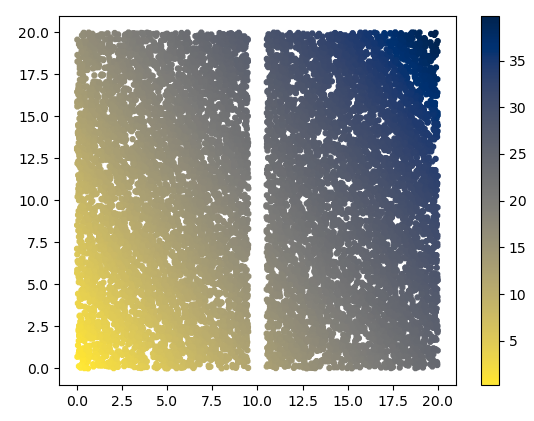
\includegraphics[width=\textwidth]{Images/Frontiere_int2_final.png}
            \caption[]%
            {{\small Échelonnage avec écart type.}}    
        \end{subfigure}
        \caption{Deux techniques de redressement (écart type différent).}
    \end{figure}

    Dans les deux cas, on se concentre sur la frontière. Si les conditions du terrain changent la variation des mesures, prendre en compte l'écart type permet de gommer une bonne partie de l'erreur obtenue. En revanche, le modèle linéaire ne peut faire qu'approcher la réalité du terrain. Calculer les termes de plus haut degré (carré, cube) serait bien plus complexe pour un gain peu significatif (en témoigne du redressement sur (\ref{2_avant_apres})).    

\newpage
\subsection{Gestion des données manquantes et redressement des positions}\label{2-don_manq}

    Lors de la récolte sur le terrain, il peut arriver que la localisation de l'appareil plante. Dans ce cas, un certain nombre de points se retrouve sans position ni temps associé (champs NaN, Not a Number).

    La solution la plus simple dans ce cas est de les supprimer complètement. En général, le géophysicien ne continue pas l'acquisition de donnéessur la zone et se contente simplement de terminer le profil en cours. Perdre les points défectueux ne constitue donc pas une perte majeur. En revanche, l'appareil continue de mesurer le sol avec ses bobines ; il n'est donc pas inutile de vouloir conserver ces mesures dans l'analyse.

    Cependant, comme indiqué précedemment, il peut être compliqué de les utiliser au vu des coordonnées manquantes. Elles sont nécessaires au traitement. La seule solution est donc de les estimer à l'aide des autres points du jeu de données.

    Une première partie de la question a déjà été résolue, celle d'identifier les différents profils. Cela servait à l'origine à séparer les points de la base du reste des mesures. Grâce à cela on peut identifier quels points peuvent servir à redresser les données manquantes, sous certaines hypothèses : 

    \begin{enumerate}
        \item[\textbf{(1)}] Une série de points manquants appartient toujours au même profil, et sont situés à la fin de celui-ci. Cette hypothèse est raisonnable compte tenu des précautions prises par le géophysicien en cas de déconnexion.
        \item[\textbf{(2)}] Les points en base sont toujours correctement définis (ce qui rejoint le premier point).
        \item[\textbf{(3)}] Un profil est toujours effectué le plus linéairement possible. On peut donc imaginer que les positions manquantes se trouvent sur la continuation d'une droite formée par les autres points du profil.
        \item[\textbf{(4)}] La vitesse du géophysicien est constante, ainsi que l'écart de temps entre chaque mesure. Les points adjacentsd'une même profil doivent donc être en théorie équidistants.
    \end{enumerate}

    \textbf{\underline{Solution choisie :}} \textbf{Régression linéaire} : L'idée est de d'abord détecter chaque bloc NaN. On détecte ensuite leur profil associé en se basant sur le point précédent dans le jeu de données (classés par ordre chronologique) (hypothèses \textbf{(1)} et \textbf{(2)}).
    
    On sélectionne l'ensemble des points connus de même profil, puis on effectue une régression linéaire sur les axes X et Y, ainsi que sur le temps (hypothèse \textbf{(3)}). Compte tenu de l'hypothèse \textbf{(4)}, il est possible de prendre comme ordonnée des régressions l'indice du point dans le fichier. Chacune des trois régressions est indépendante.
    
    \label{2_Na_compl_out}Il suffit enfin de prédire la donnée recherché avec l'indice en se basant sur les constantes de la régression. La procédure est en $O(n)$ (\ref{2_Na_compl_in}).\\

    \begin{figure}[ht!]
        \centering
        \begin{subfigure}[b]{0.475\textwidth}
            \centering
            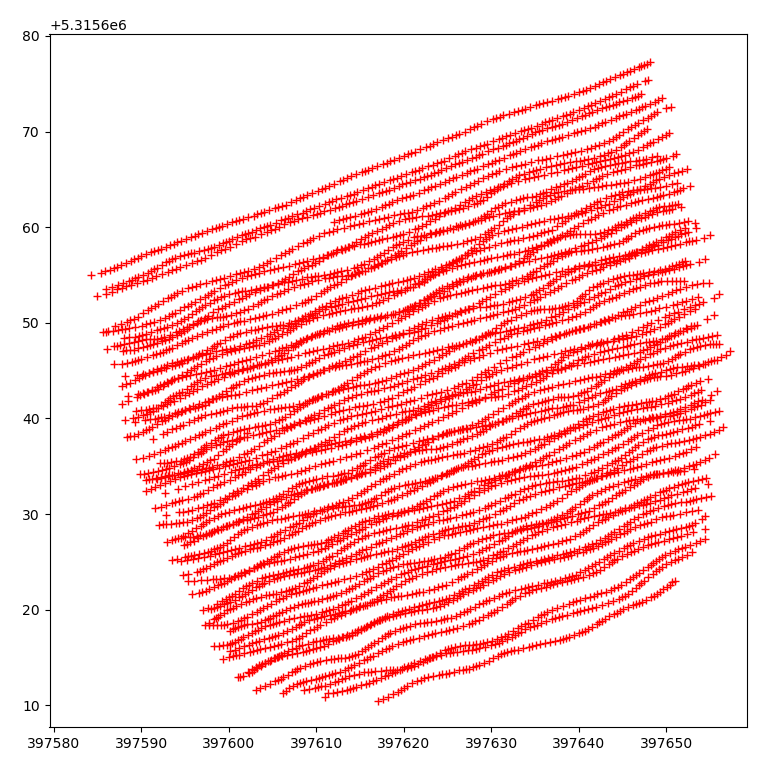
\includegraphics[width=\textwidth]{Images/Na_Avant2.png}
            \caption[]%
            {{ \small Jeu après retrait des points NaN.}}    
        \end{subfigure}
        \hfill
        \begin{subfigure}[b]{0.475\textwidth}  
            \centering 
            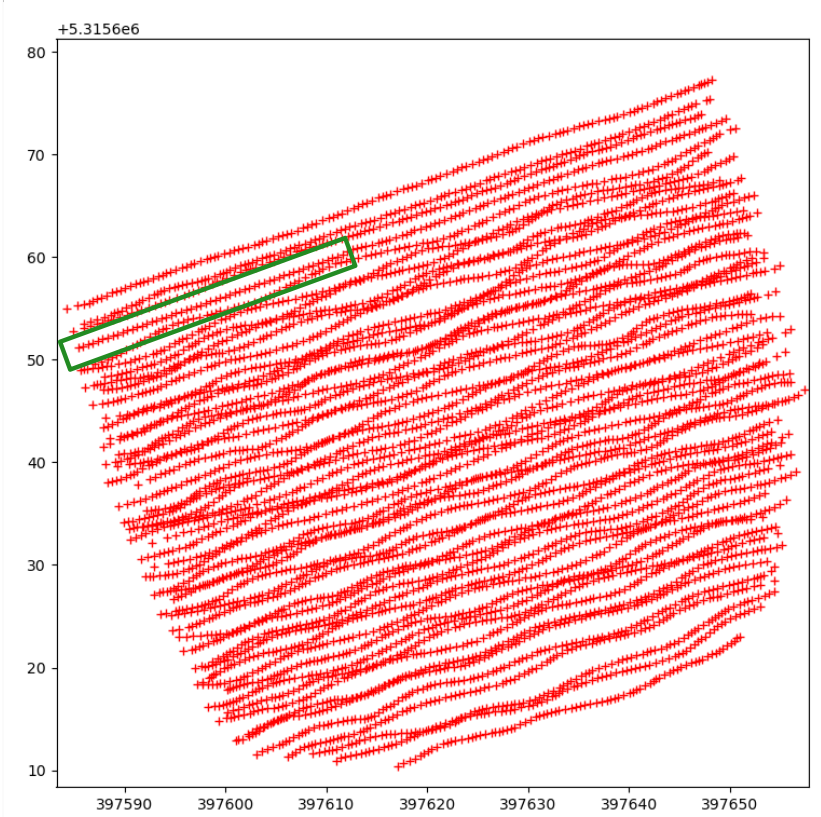
\includegraphics[width=\textwidth]{Images/Na_Apres2.png}
            \caption[]%
            {{\small Jeu après correction NaN.}}    
        \end{subfigure}
        \caption{Recalibrage des points incomplets (en vert).}
    \end{figure}
    
    \label{2_regr_compl_out}Cette solution permet de résoudre un autre problème sur les positions. On remarque sur le jeu précédent que les profils sont sinusoïdaux, ce qui correspond à une erreur de localisation GPS. Lorsque celle-ci est trop prononcée (comme ici), elle bruite le jeu de manière significative. Mais en effectuant les régressions sur tous les profils, on peut projeter les coordonnées de tous les points sur une droite. (\ref{2_regr_compl_in})

    On préfèrera ne pas appliquer cette transformation sur tous les jeux de données, car la plupart du temps le décalage correspond à la réelle trajectoire du géophysicien. On crée donc une erreur pas toujours nécessaire. On pourrait aussi vouloir restreindre l'opération à un ensemble de profils. Il sera donc important de laisser la main à l'utilisateur dans le choix de la meilleure méthode.

    \begin{figure}[ht!]
        \centering
        \begin{subfigure}[b]{0.475\textwidth}
            \centering
            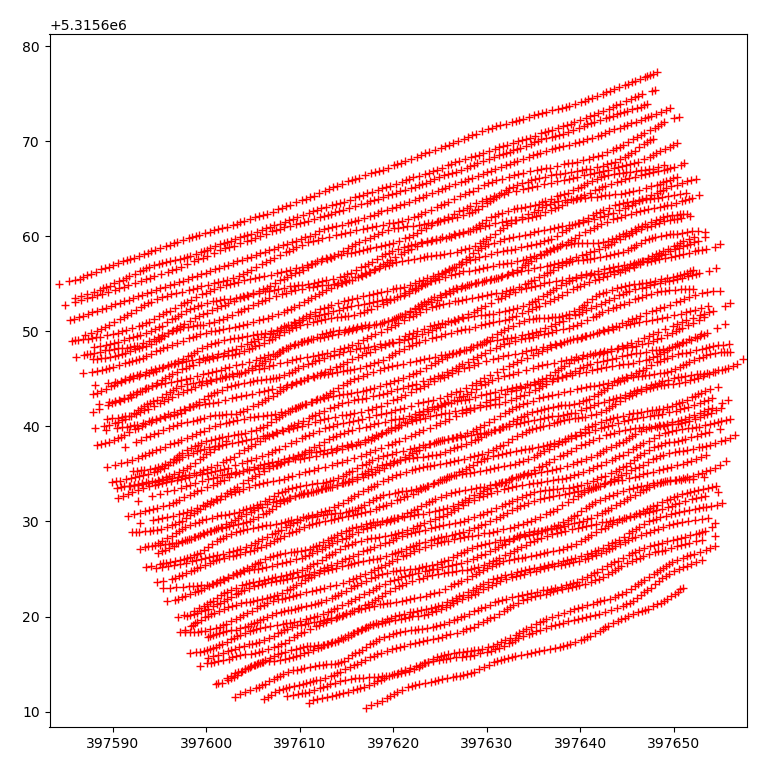
\includegraphics[width=\textwidth]{Images/Regr_Avant2.png}
            \caption[]%
            {{ \small Jeu après correction NaN.}}    
        \end{subfigure}
        \hfill
        \begin{subfigure}[b]{0.475\textwidth}  
            \centering 
            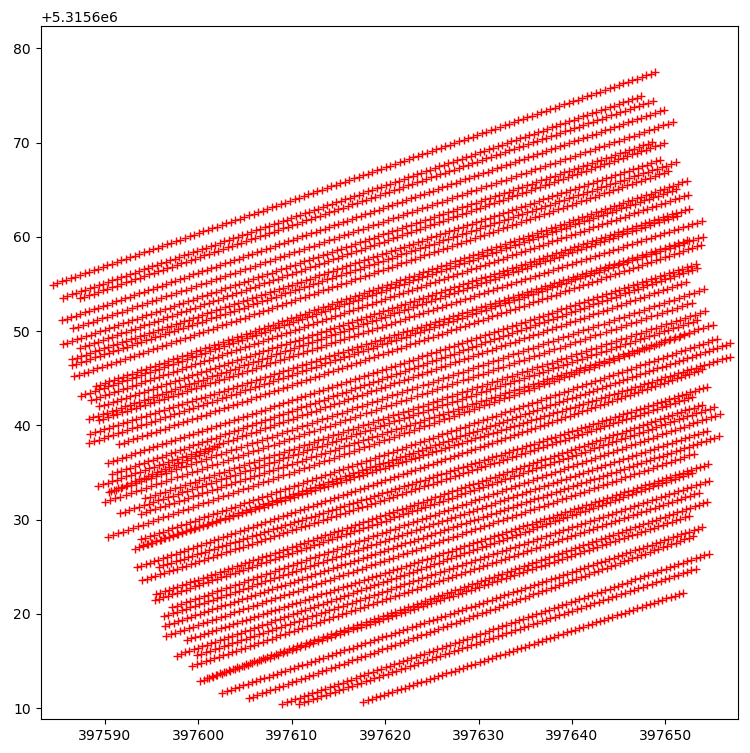
\includegraphics[width=\textwidth]{Images/Regr_Apres2.png}
            \caption[]%
            {{\small Jeu après régression sur l'ensemble.}}    
        \end{subfigure}
        \caption{Réalignement des profils.}
    \end{figure}

\newpage\newpage
    Il existe cependant des types de prospections faites au point par point, c'est-à-dire que l'utilisateur parcourt le terrain sans nécessairement passer par des trajectoires rectilignes. De plus, la prise des points peut être faite en continu. Tout cela peut empêcher de se référer à une division de la prospection par profil.

    \label{2_Na_compl_solo_out} Dans ce cas, on pourra établir la completion des points NaN en traçant une droite entre les points connus avant et après et en y reportant les points inconnus. Cette solution est moins coûteuse en hypothèse, mais risque de créer plus d'erreurs de positionnement puisqu'on ne se base que sur deux points (\ref{2_Na_compl_solo_in}).

    Sur l'exemple suivant, on remarque que la répartition des points n'est rectiligne que sur une partie de l'ensemble. On ne pourra pas modéliser le nuage en bas à gauche par des profils linéaires. Par conséquent, on pourra rectifier chaque point séparément.

    On vérifie sur la figure de droite que les points ajoutés s'intègrent correctement à la structure du nuage de points.

    \begin{figure}[ht!]
        \centering
        \begin{subfigure}[b]{0.475\textwidth}
            \centering
            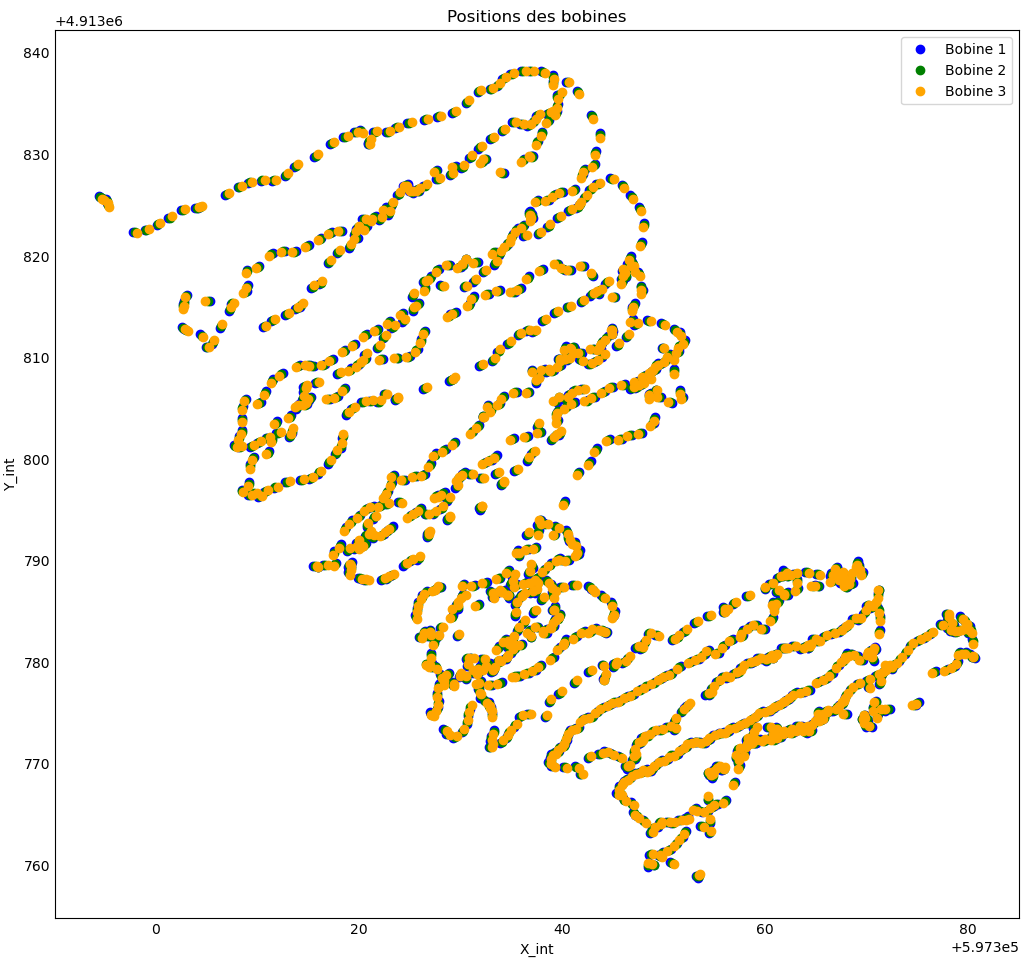
\includegraphics[width=\textwidth]{Images/NA_solo_Avant.png}
            \caption[]%
            {{ \small Jeu après retrait des points NaN.}}    
        \end{subfigure}
        \hfill
        \begin{subfigure}[b]{0.475\textwidth}  
            \centering 
            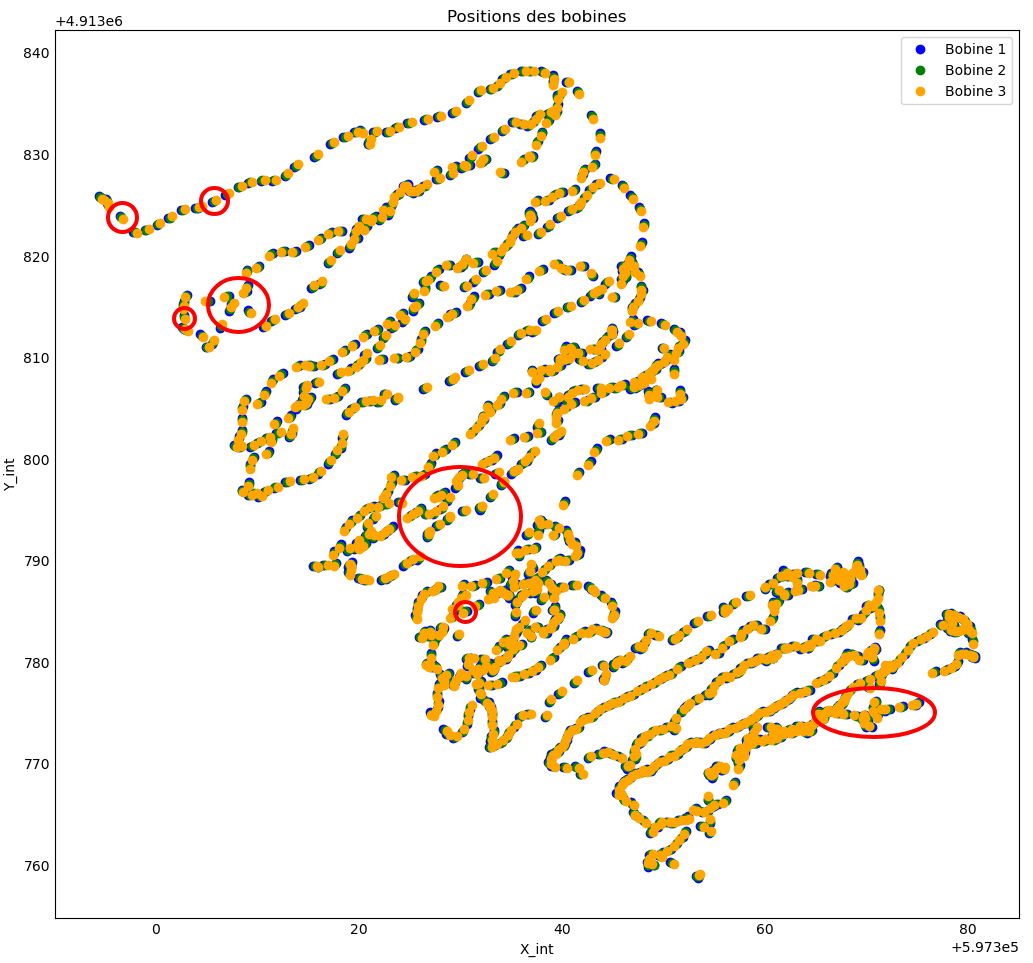
\includegraphics[width=\textwidth]{Images/NA_solo_Apres.png}
            \caption[]%
            {{\small Jeu après correction NaN.}}    
        \end{subfigure}
        \caption{Complétion au point par point.}
    \end{figure}

    Le représentation ci-dessus suit la procédure décrite dans la partie suivante.

\newpage
\subsection{Division des positions par bobine} \label{2-divpos}

    Une des erreurs que possède la position (GPS ou non) mesurée par l'appareil, c'est qu'elle ne prend pas en compte la différence de position du centre de chaque couples de bobines pour un même point de prospection. Afin de réduire ce biais, on effectue un recalibrage où chaque voie aura son propre X et Y.

    On se place dans le système d'hypothèse suivant :

    \begin{enumerate}
        \item[\textbf{(1)}] L'appareil garde la même répartition de bobine, c'est-à-dire que les écarts émetteur/récepteur sont constants.
        \item[\textbf{(2)}] Le sens dans lequel l'appareil est tourné est constant par rapport au sens de marche.
        \item[\textbf{(3)}] La trajectoire entre deux point mesurés est linéaire.
    \end{enumerate}

    On doit donc tout d'abord obtenir l'information de la position des bobines par rapport au centre de l'appareil. On prendra le repère $O_{lt}$, où $l$ est l'axe de déplacement dans le sens de la marche et $t$ est l'axe perpendiculaire à $l$ formant un repère orthonormé.

    \begin{figure}[ht!]
        \centering
        \begin{subfigure}[b]{0.475\textwidth}
            \centering
            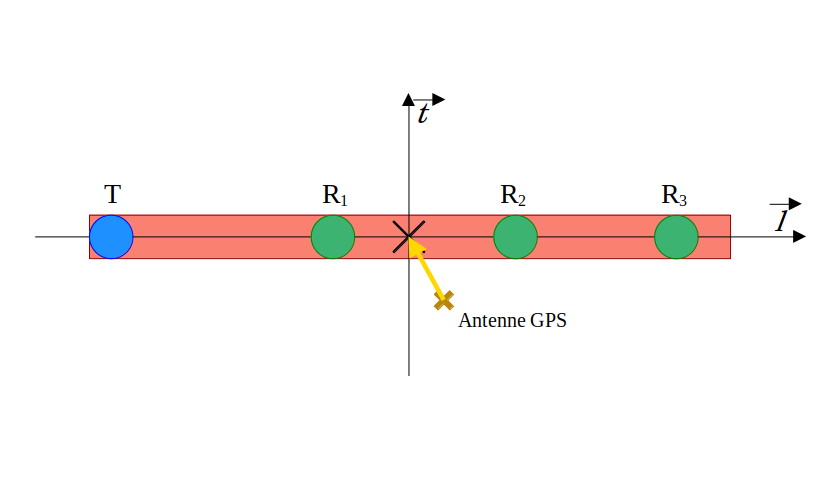
\includegraphics[width=\textwidth]{Images/SepVoies_Sch1.png}
            \caption[]%
            {{ \small Appareil dans le sens de la marche.}}    
        \end{subfigure}
        \hfill
        \begin{subfigure}[b]{0.475\textwidth}  
            \centering 
            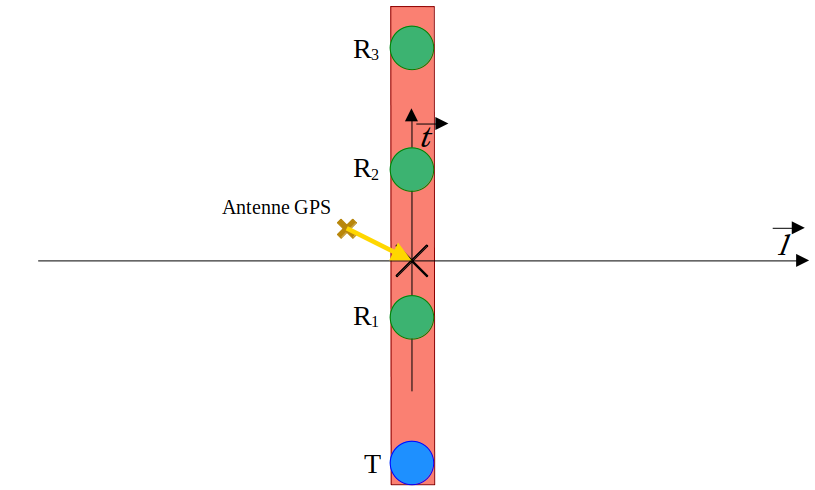
\includegraphics[width=\textwidth]{Images/SepVoies_Sch2.png}
            \caption[]%
            {{\small Appareil incliné.}}    
        \end{subfigure}
        \caption{Schéma de la position des bobines dans le repère.}
    \end{figure}

    Chaque bobine sera donc représenté par deux coordonnées. En l'occurence, on se réfère aux paramètres \texttt{TR\_l} et \texttt{TR\_t} de l'appareil (\ref{2-app}).

    De plus on prend en compte le décalage de l'antenne GPS avec le paramètre \texttt{GPS\_dec}. Si aucune antenne n'est utilisée (pas de GPS), on considérera ce décalage comme nul.

    Ensuite, en suivant l'ordre dans lequel les points ont été mesurés (et en prenant en compte le début/fin des profils), on peut déduire l'angle de déplacement dans le repère X/Y des coordonnées mesurées. On peut donc appliquer ensuite une translation sur chaque bobine en tout point du jeu.

    \begin{figure}[ht!]
        \begin{center}
            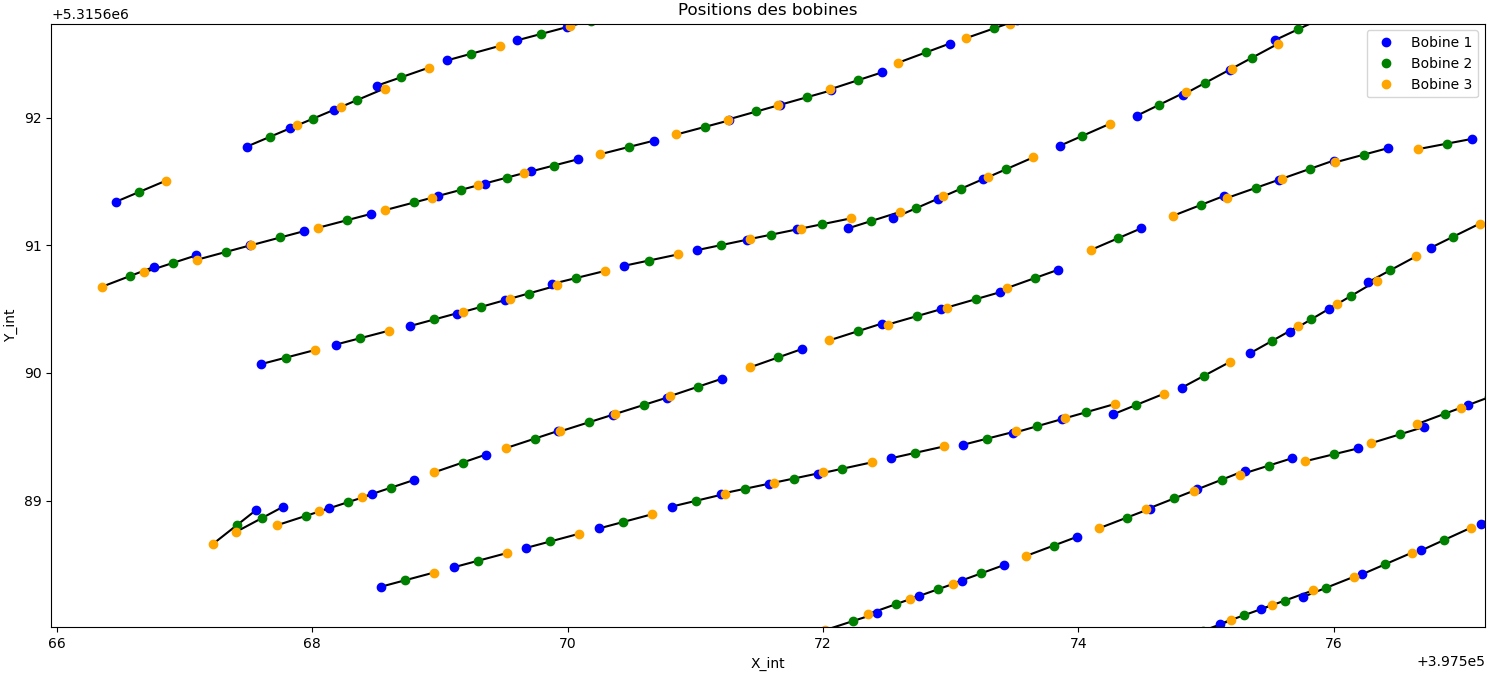
\includegraphics[width=0.90\textwidth]{Images/SepVoies_plot.png}
            \caption{Positions des bobines sur quelques morceaux de profils}
        \end{center}
    \end{figure}

    On a représenté chaque voie par une couleur différente, et les trois positions appartenant à un même point sont reliés par un trait noir.

    On vérifie en premier lieu que les profils sont de sens alternés grâce à la légende. Par exemple, le premier profil (en haut) va de gauche à droite et le second de droite à gauche. De plus, les profils sont équidistants. En effet, cette représentation est cohérente avec la manière dont la cartographie a été réalisé. Enfin, on retrouve que l'appareil est parallèle à la direction d'avancement.

    De cette manière, on peut estimer que la procédure a été correctement réalisée.

    Ce seront ces nouvelles positions qui devront être utilisées pour les traîtements suivants, comme par exemple les frontières, l'étalonnage manuel ou par profil ou encore la mise en grille.

    Attention, si le nombre de points du jeu est important, cet affichage peut provoquer des lags / freezes.

    \newpage
    \subsection{Détection pseudo-profils}

    La découpage en profils est important pour permettre par la suite de corriger des déformations dû à l'appareil (la procédure en question est décrite dans la partie suivante \ref{2-etal}). Or cette information est absente du fichier de données, on doit donc la recréer. Pour cela on a besoin de procéder différemment en fonction du type de prospection réalisée.

    \begin{enumerate}
        \item[$\bullet$] Si l'appareil ne possède pas de données GPS, on est dans un cas trivial. La position (notée \texttt{"x[m]"} et \texttt{"y[m]"}) est indicative d'une cartographie en position relative (souvent par carré de prospection), où chaque profil suit l'axe $y$. Il suffit donc de commencer un nouveau profil à chaque fois que le $x$ change.
        \item[$\bullet$] Dans la majorité des cas où l'appareil utilise une antenne GPS, l'utilisateur commence par une base. Puis, il prospecte le terrain en marquant une pose entre chaque profil. Il peut de temps en temps revenir mesurer une base. Pour correctement découper la prospection en profils et bases, il faut détecter les changements brutaux de temps et surveiller si le profil trouvé est positionné au même endroit que la première base.
        \item[$\bullet$] Il peut arriver qu'une prospection utilises une antenne GPS, mais qu'elle soit réalisée sans s'arrêter. Par exemple, cela peut être le cas en mesure point par point ou sur de faibles surfaces. Dans ce cas, on ne trouvera aucun saut dans le temps. De plus, la trajectoire ne sera pas parfaitement linéaire car la jonction entre deux profils (en demi-cercle) est à prendre en compte, et on doit de toute manière pouvoir gérer des profils qui dévient de leur trajectoire.
    \end{enumerate}

    Le premier cas ne pose pas de problème particulier, et le second est déjà traité avant le stage. On va donc dans cette partie chercher une solution au troisième cas.

    En particulier on fait les tests sur les deux cas problématiques suivants :

    \begin{figure}[ht!]
        \centering
        \begin{subfigure}[b]{0.475\textwidth}
            \centering
            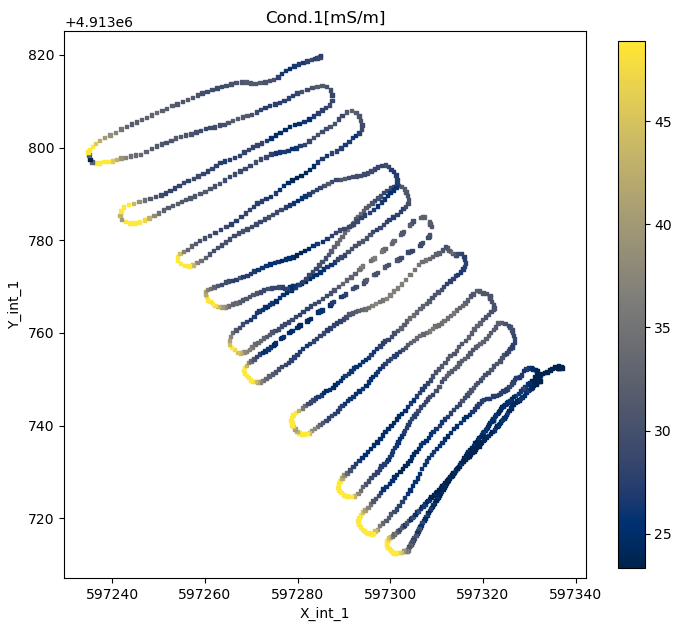
\includegraphics[width=\textwidth]{Images/PseudoProf_1.png}
            \caption[]{{ \small Profils clairs avec virages.}}    
            \label{fig:2_pp_1}
        \end{subfigure}
        \hfill
        \begin{subfigure}[b]{0.475\textwidth}  
            \centering 
            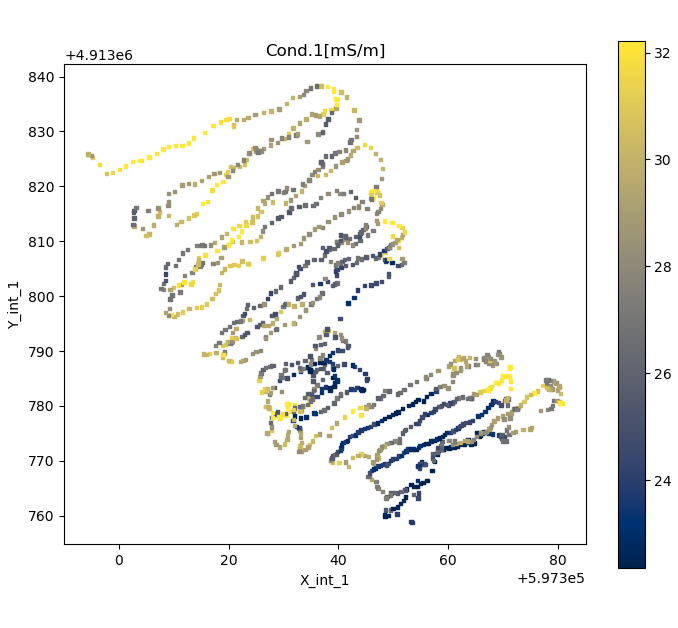
\includegraphics[width=\textwidth]{Images/PseudoProf_2.png}
            \caption[]{{\small Profils chaotiques à tailles variables.}}    
        \end{subfigure}
        \caption{Différents exemples à régler.}
    \end{figure}

    Puisque la définition de profils est ambigü au vu de leur possible non linéarité, on parlera plutôt de pseudo-profils.

    \noindent\textbf{\underline{Solution envisagée}} :
    \begin{enumerate}
        \item[$\bullet$] \textbf{Points à intervalles réguliers} : Au lieu de chercher à se reporter à des pseudo-profils, on pourrait choisir de prendre un point par intervalle régulier (1 point tous les 50 par exemple) ou à proportion régulière (50 points répartis proportionnellement). Déterminer de tels points ne nécessite aucun calculs particulier, et on pourra alors choisir la médiane sur le voisionnage des points pour être représentatif de la zone choisie. Malheureusement, cette solution est inexploitable à cause de la déformation du terrain. Il n'est pas possible de faire la différence entre le terrain et le biais de l'appareil. par exemple sur le jeu \ref{fig:2_pp_1}, la partie gauche va fausser la mesure.
    \end{enumerate}
    \textbf{\underline{Solution choisie}} : \textbf{Centres de profils} : \label{2_pseudoprof_out} On cherche à déduire le centre des profils sans aucune information de départ. Si on y arrive, alors on pourra associer chaque point à un centre en fonction de l'ordre de prospection et donc recréer un découpage se rapprochant d'un profil. (\ref{2_pseudoprof_in})

    \subsubsection{Régression linéaire}

    Afin d'estimer les centres des profils, on souhaite déterminer une droite passant par les centres par régression. Une fois fait, on pourra calculer la distance à la droite en tout point du jeu de données.

    La forme la plus évidente pour cela est de passer par une équation de droite de la forme $ax + by + c = 0$. Cependant, une régression classique de $y$ par rapport à $x$ ne donne pas cette information, car les coefficients $slope$ et $intercept$ trouvés correspondent à une forme $y = slope*x + intercept$, plus restrictive. Par exemple une droite d'équation $x = 5$ n'est pas représentable sous cette forme.

    Par conséquent, on utilise un raisonnement similaire à la partie sur la complétion NaN (\ref{2-don_manq}). On effectue une régression linéaire sur l'indice des lignes et $x$ et $y$. De cette manière, on obtient les 4 constantes répondant au système suivant :

    \begin{spacing}{1}
        \begin{equation}
            \scalebox{1.25}{$
            \begin{cases}
                x = a_xi + b_x \\
                \\
                y = a_yi + b_y
            \end{cases}
            $}
        \end{equation}
    \end{spacing}
    
    où $i$ est l'indice des lignes et $a_x$,$a_y$,$b_x$,$b_y$ les constantes des deux régressions. On cherche ensuite à retirer $i$ du calcul pour ne laisser que $x$ et $y$ en ligne de compte. Pour cela, on exprime $i$ en fonction des deux autres :

    \begin{spacing}{1}
        \begin{equation}
            \scalebox{1.25}{$
            \begin{cases}
                i = \frac{x - b_x}{a_x} \\
                \\
                i = \frac{y - b_y}{a_y}
            \end{cases}
            $}
        \end{equation}
    \end{spacing}

    La relation finale doit être une droite, donc on au moins l'un de $a_x$ et $a_y$ est non nul (sinon le résultat est un point). Le système étant symétrique, on pourra choisir la relation que l'on veut. Pour l'exemple prenons la première :

    \begin{spacing}{1}
        \begin{equation}
            \scalebox{1.25}{$y = a_y\frac{x - b_x}{a_x} + b_y$}
            \implies
            \scalebox{1.25}{$y = \frac{a_y}{a_x}x - \frac{a_y}{a_x}b_x + b_y$}
        \end{equation}
        \begin{equation}
            \implies
            \scalebox{1.25}{$a_xy - a_yx + b_xa_y - b_ya_x = 0$}
        \end{equation}
        \begin{equation}
            \implies
            \scalebox{1.25}{$\textcolor{red}{a_y(x - b_x) - a_x(y - b_y) = 0}$}
        \end{equation}
    \end{spacing}

    On obtient une équation de droite exploitable. On cherche maintenant à établir une distance point/droite. La distance effective est calculée selon \href{https://fr.wikipedia.org/wiki/Distance_d%27un_point_%C3%A0_une_droite#Dans_le_plan}{la relation suivante} :

    \begin{spacing}{1}
        \begin{equation}
            \scalebox{1.25}{$d = \frac{|a_y(x - b_x) - a_x(y - b_y)|}{\sqrt{a_x^2 + a_y^2}}$}
        \end{equation}
    \end{spacing}

    Puisqu'on cherche à comparer les distances, on peut ignorer le terme constant au dénominateur, ce qui laisse simplement à calculer la valeur absolue du terme de l'équation de droite, à savoir.

    \begin{spacing}{1}
        \begin{equation}
            \scalebox{1.25}{$\textcolor{red}{\delta = |a_y(x - b_x) - a_x(y - b_y)|}$}
        \end{equation}
    \end{spacing}

    Pour s'en assurer, on vérifie la conservation des ratios entre $d$ et $\delta$ :

    \begin{spacing}{1}
        \begin{equation}
            \scalebox{1.25}{$\frac{\delta_1}{\delta_2} = \frac{\delta_1}{\delta_2}\frac{\sqrt{a_x^2 + a_y^2}}{\sqrt{a_x^2 + a_y^2}} = \frac{\frac{\delta_1}{\sqrt{a_x^2 + a_y^2}}}{\frac{\delta_2}{\sqrt{a_x^2 + a_y^2}}} = \frac{d_1}{d_2}$}
        \end{equation}
    \end{spacing}

    Ce calcul est très rapide à effectuer.
    
    Pour déterminer quels sont les centres des profils, on choisira les minimums locaux de l'évolution des distances. En revanche, ce critère seul ne suffit pas. Les irrégularités des profils créent des minimums locaux éloignés de la courbe, en témoigne leur présence en dehors des creux.
    
    \begin{figure}[ht!]
        \centering
        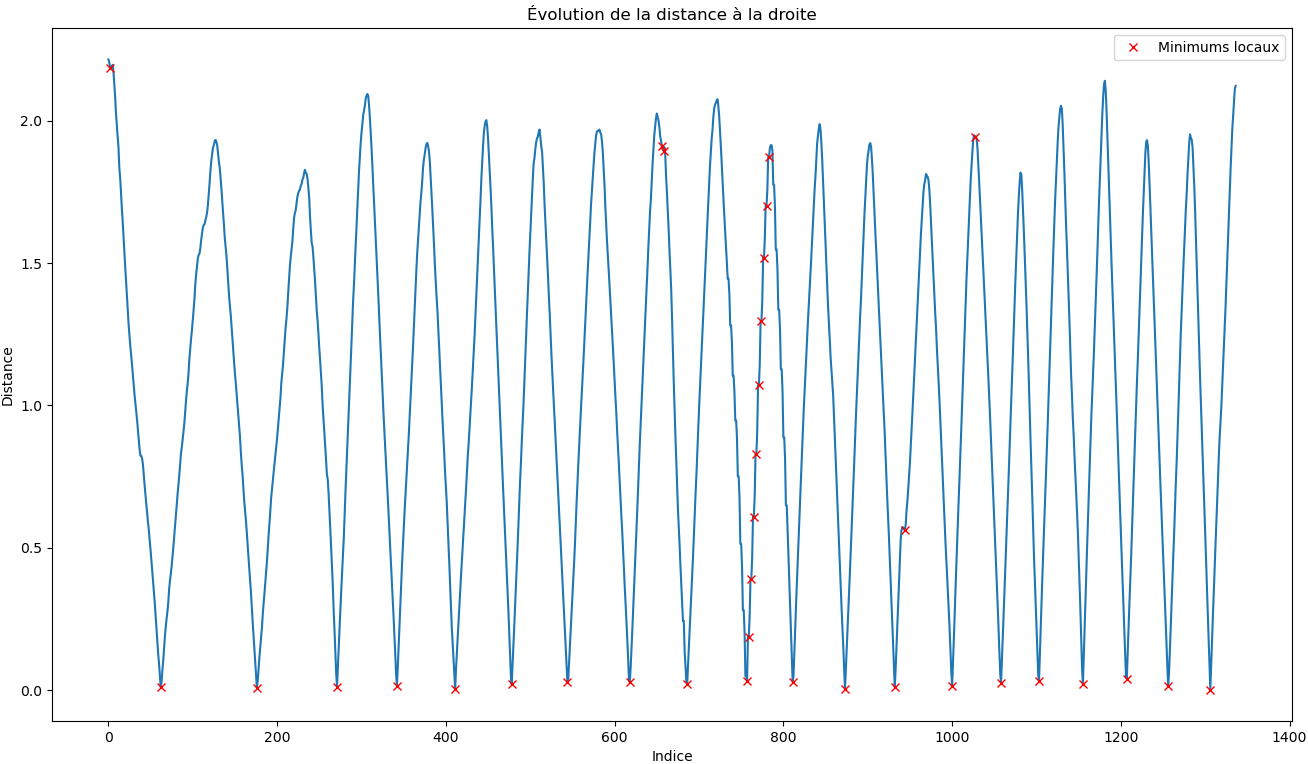
\includegraphics[width=\textwidth]{Images/PseudoProf_dist_1.png}  
        \caption{Évolution de la distance à la droite par rapport à l'indice, jeu 1.}
    \end{figure}

    On doit donc éliminer ensuite ces points. On prend comme valeur de seuil \texttt{tn\_c = 20} fois la moyenne des \texttt{tn = 10} points à distance minimale, en supposant qu'une prospection devrait comprendre au moins 10 profils (et donc au moins 10 points très proches de la droite).

    Malgré cela, il existe deux derniers cas gênant. En premier lieu, celui de détecter deux fois le même profil.
    
    \begin{figure}[ht!]
        \centering
        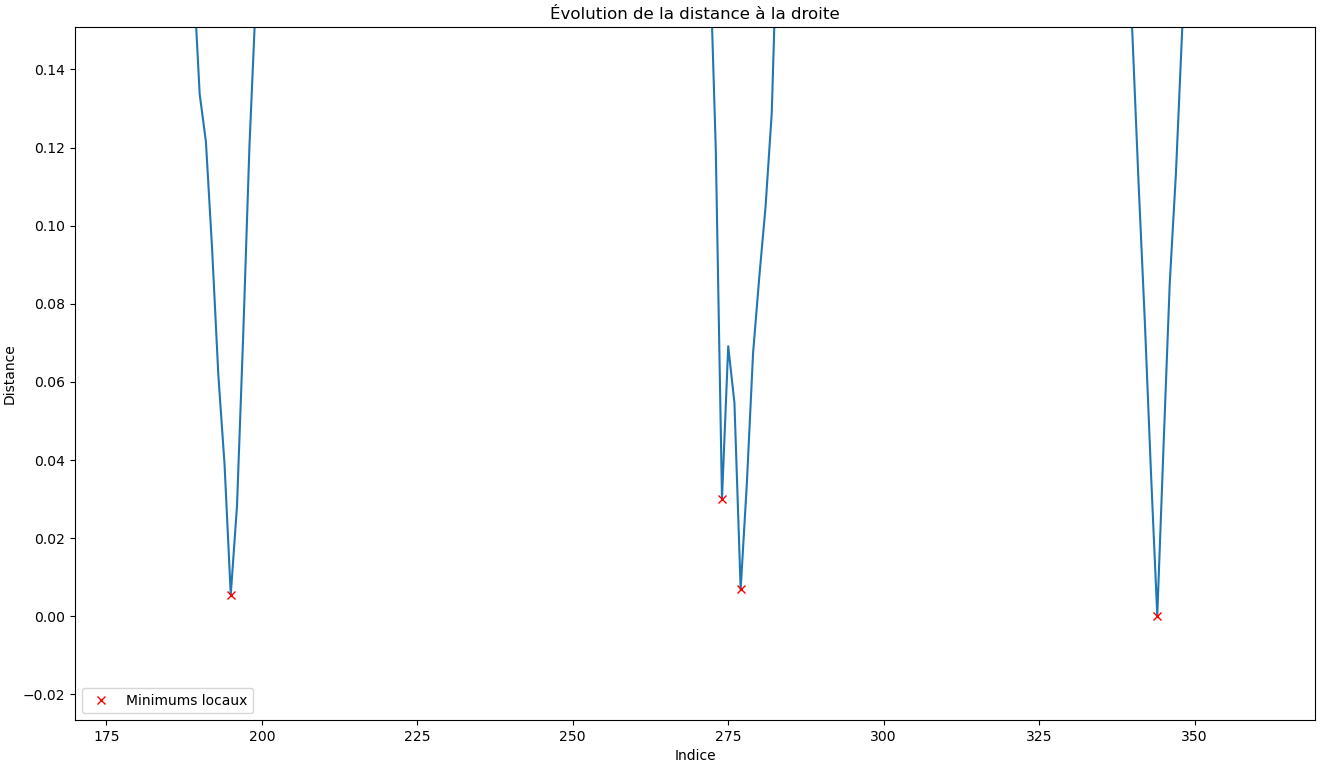
\includegraphics[width=\textwidth]{Images/PseudoProf_dist_2.png}  
        \caption{Extrait de l'évolution de la distance à la droite par rapport à l'indice, jeu 2.}
    \end{figure}

    Si deux points sont espacés de moins de \texttt{min\_conseq = 8} en indice, le plus éloigné sera retiré. On considère qu'un profil devrait mesurer au moins 8 points et que si deux points sont plus espacés, alors au moins l'un d'entre eux sera suffisament excentré pour être éliminé suite au premier filtre. Si un profil revient sur ses pas après plus de 8 points, la procédure va le considérer comme deux profils distincts.

    En second lieu, si certains profils sont trop éloignés de la droite des centres, il est possible qu'il ne se touchent pas. Dans ce cas, on mesurera des profils bien trop grand qui en sont en réalité plusieurs. Par conséquent, si deux centres sont plus éloignés que le double de la médiane des écarts, on coupera la zone entre les deux en insérant des centre arbitraires.

    Enfin, pour chaque point du jeu, on lui associe le centre trouvé le plus proche. L'indice de ce centre dans la liste des centres permettra de numéroter le profil.

    \newpage
    Résultat :
    \begin{figure}[ht!]
        \centering
        \begin{subfigure}[b]{0.90\textwidth}
            \centering
            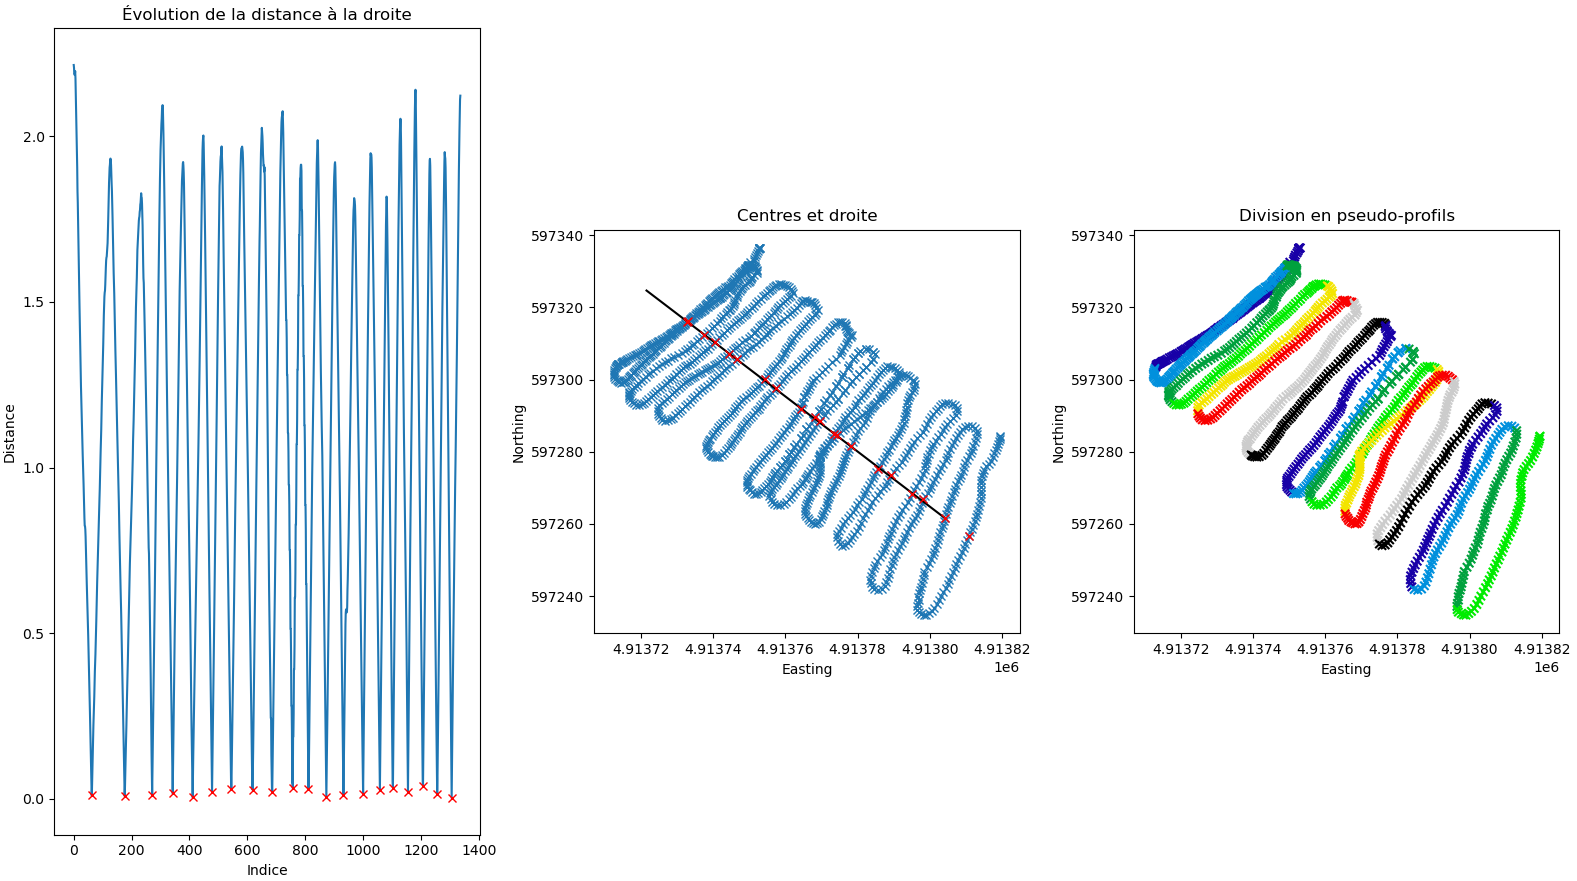
\includegraphics[width=\textwidth]{Images/PseudoProf_full_1.png}
            \caption[]%
            {{ \small Jeu 1 (facile).}}    
        \end{subfigure}
        \centering
        \begin{subfigure}[b]{0.90\textwidth}  
            \centering 
            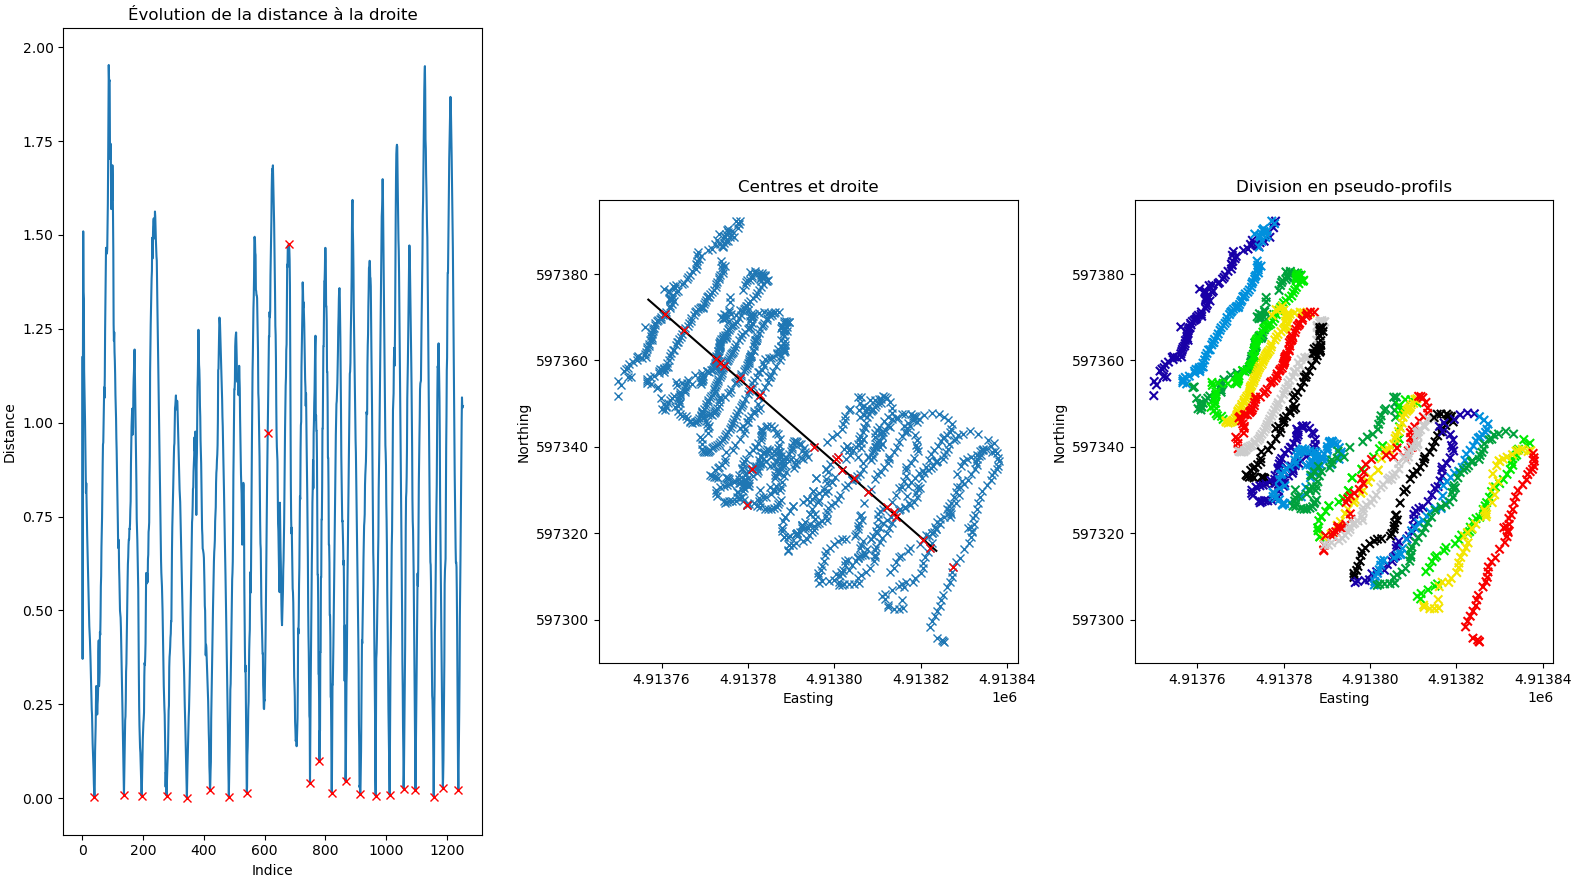
\includegraphics[width=\textwidth]{Images/PseudoProf_full_2.png}
            \caption[]%
            {{\small Jeu 2 (difficile).}}   
            \label{fig:2_pp_2}
        \end{subfigure}
        \caption{Découpage en pseudo-profils proposé.}
    \end{figure}

    \newpage
    \subsubsection{Découpage en segments}

    On remarque sur la figure \ref{fig:2_pp_2} que le découpage du bloc en bas à gauche n'est pas optimal, et qu'on aimerait que la droite coupe ses profils. Dans ce cas, il est intéressant de considérer une succession connexe de segments pour le calcul de la distance. De cette manière on peut s'assurer que tous les profils sont traversés.

    Les $n$ segments seront construits avec les coordonnées de $n+1$ points spécifiés par l'utilisateur. On s'assure donc d'avoir en entrée au moins deux points.

    Afin de calculer la distance entre un point $p$ et un segment $[A,B]$, on effectue un test sur les angles $\widehat{pAB}$ et $\widehat{pBA}$. On suit la procédure suivante :

    \begin{spacing}{1}
        \begin{equation}
            \scalebox{1.25}{$
            \begin{cases}
                \widehat{pAB} > 90° \implies d = ||\overrightarrow{pA}|| \\
                \widehat{pBA} > 90° \implies d = ||\overrightarrow{pB}|| \\
                sinon \implies d = \frac{||\overrightarrow{AB}\land\overrightarrow{Ap}||}{||\overrightarrow{AB}||}
            \end{cases}
            $}
        \end{equation}
    \end{spacing}

    On réalise le calcul pour chaque segment et on garde le minimum. On a donc un nouveau calcul de distance (cette fois-ci exact).

    Puisque les segments en entrée sont censés traverser tous les profils (sinon le choix n'a pas d'intérêt), on ignore la procédure de rajout de centres sur grands blocs.

    \begin{figure}[ht!]
        \centering
        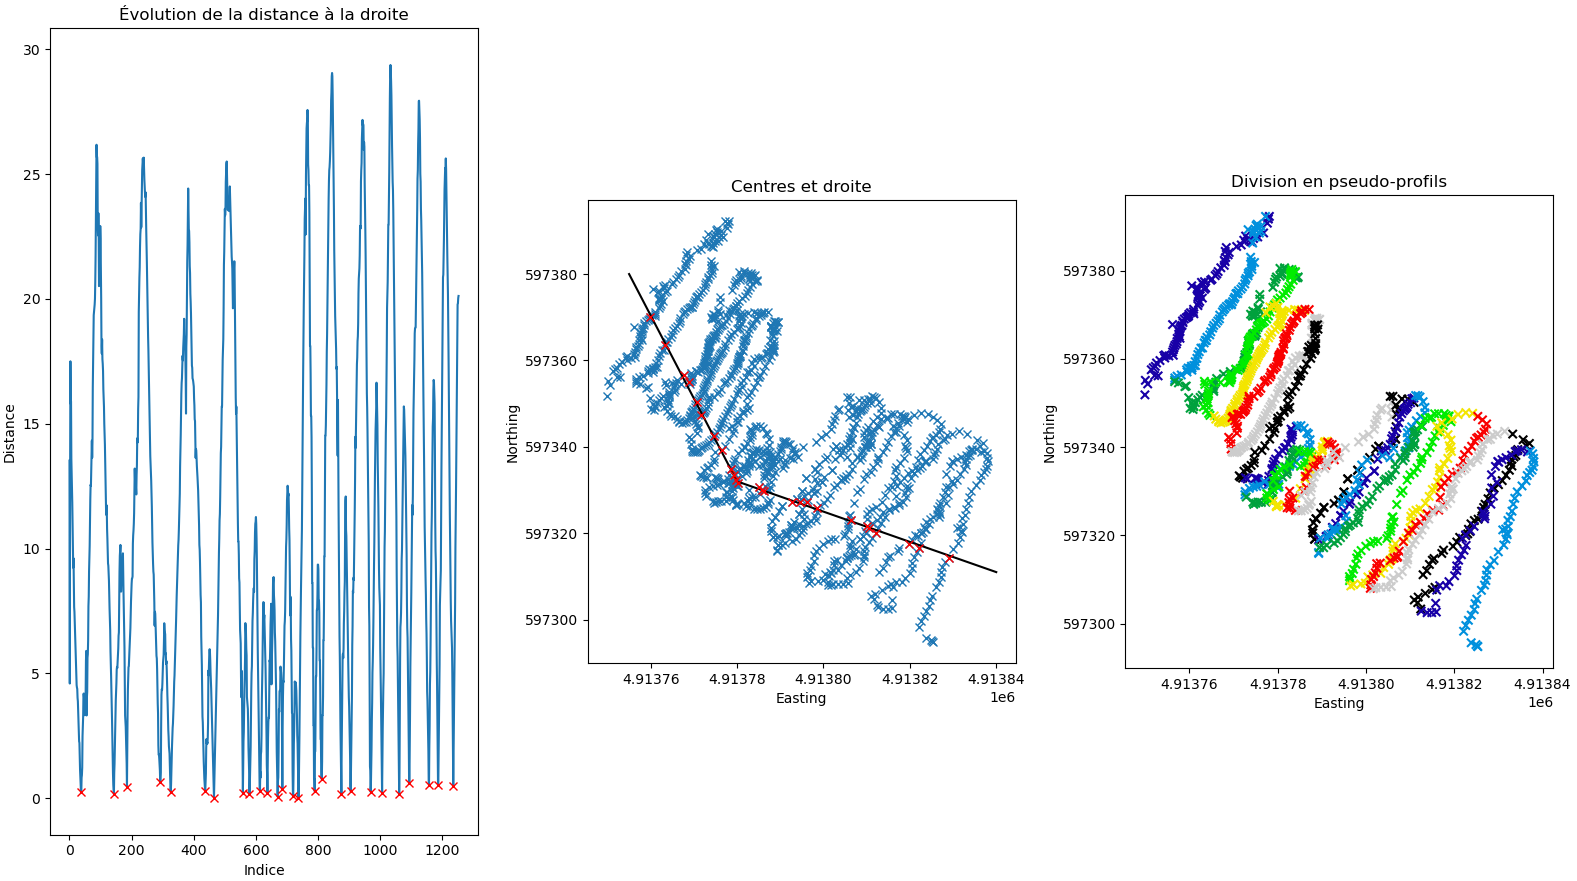
\includegraphics[width=\textwidth]{Images/PseudoProf_full_2_seg.png}  
        \caption{Découpage en pseudo-profils proposé, jeu 2.}
        \label{fig:2_pp_2_seg}
    \end{figure}

    \subsubsection{Remarques sur la procédure}

    Cet algorithme utilise des valeurs arbitraires pour retirer certains minimums locaux de la liste des centres. Les valeurs associées aux paramètres \texttt{tn}, \texttt{tn\_n} et \texttt{min\_conseq} ne peuvent pas couvrir tous les cas. Si le résultat est imparfait, on pourra les faire varier. Par exemple, si trop de centres sont retirés, il faut augmenter \texttt{tn} et/ou \texttt{tn\_n}.

    Sur la figure \ref{fig:2_pp_2_seg}, certains profils ne sont pas coupés en leur centre. Cependant, on associe à chaque point le centre trouvé \textit{le plus proche} dans le sens des indices lors de la numérotation des profils. Si un profil est coupé par le côté, le précédent et le suivant le sont aussi (selon toute probabilité). Or puisque les profils alternent de sens, le découpage reste tout aussi correcte.

    \begin{figure}[ht!]
        \centering
        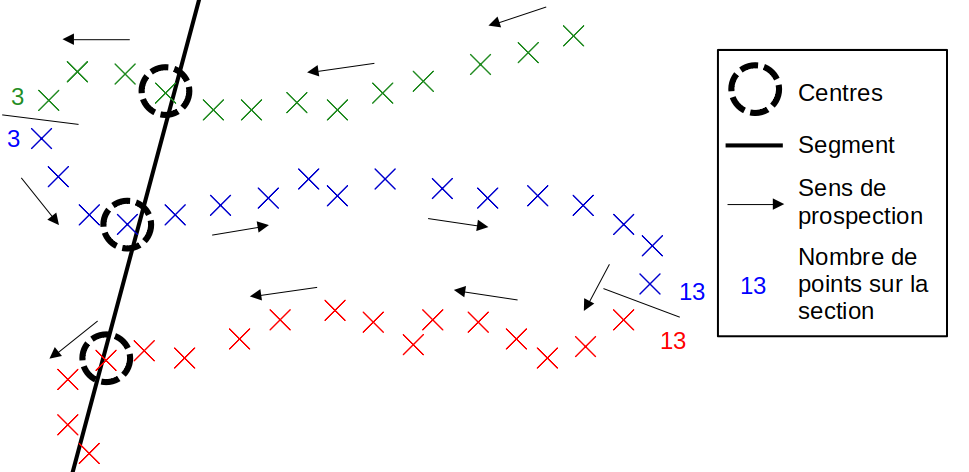
\includegraphics[width=\textwidth]{Images/PseudoProf_sch.png}  
        \caption{Stabilité de la procédure.}
    \end{figure}

    Lors de la construction de la droite ou des segments, il faut éviter de couper parallèlement à une partie d'un profil, au risque de créer pleins de centres . Dans ce cas, il est préférable de simplement changer la position des points des segments.
    
\newpage  
\subsection{Étalonnage des profils}\label{2-etal}
\subsubsection{Méthode utilisée pour l'étalonnage par base}

    \label{2_evol_base} Dans une partie précédente, nous avons tenté de corriger les erreurs entre différentes parcelles en se basant uniquement sur la frontière. Cela permet de répondre au problème de discontinuité, mais ne peut traiter les décalages survenant pendant la prospection d'une même parcelle, typiquement à cause de la dérive de instrumentent de mesure. Pour cela, on réalise des bases à des points fixes de l'espace qui serviront à uniformiser les données. Puisque qu'un même point doit donner la même valeur, on peut alors mesurer le décalage de l'appareil, à condition de revenir plusieurs fois dessus. Il s'agit d'une stratégie assez proche de celle de la frontière, mais au milieu d'une même prospection.

    Une base est constitué de plusieurs points, certains pris au sol (comme pour la prospection) ou en l'air (pour évaluer l'offset de l'appareil). On va d'abord s'ntéresser uniquement aux mesures en l'air. Tout comme les profils, une série de point en base fait partie d'une même base. Pour obtenir une valeur significative, on prendra la médiane de chaque base en compte. En parallèle, on va également calculer la médiane de chaque profil pour chaque variable observée.

    On rappelle les hypothèses du modèle :
    \begin{enumerate}
        \item[\textbf{(1)}] Plusieurs mesures de base, si situées au même endroit, doivent donner les mêmes résultat. Si ce n'est pas le cas, on considère que la différence trouvée doit être corrigée car elle vient de l'appareil.
        \item[\textbf{(2)}] Les profils et les bases au sein d'une même prospection sont établis à intervalle régulier.
        \item[\textbf{(3)}] La médiane d'un profil ou d'une base est suffisament repésentative pour pouvoir établir une évolution temporelle.
        \item[\textbf{(4)}] Un décalage survenant entre deux bases évolue de manière linéaire.
    \end{enumerate}

    \begin{figure}[ht!]
        \centering
        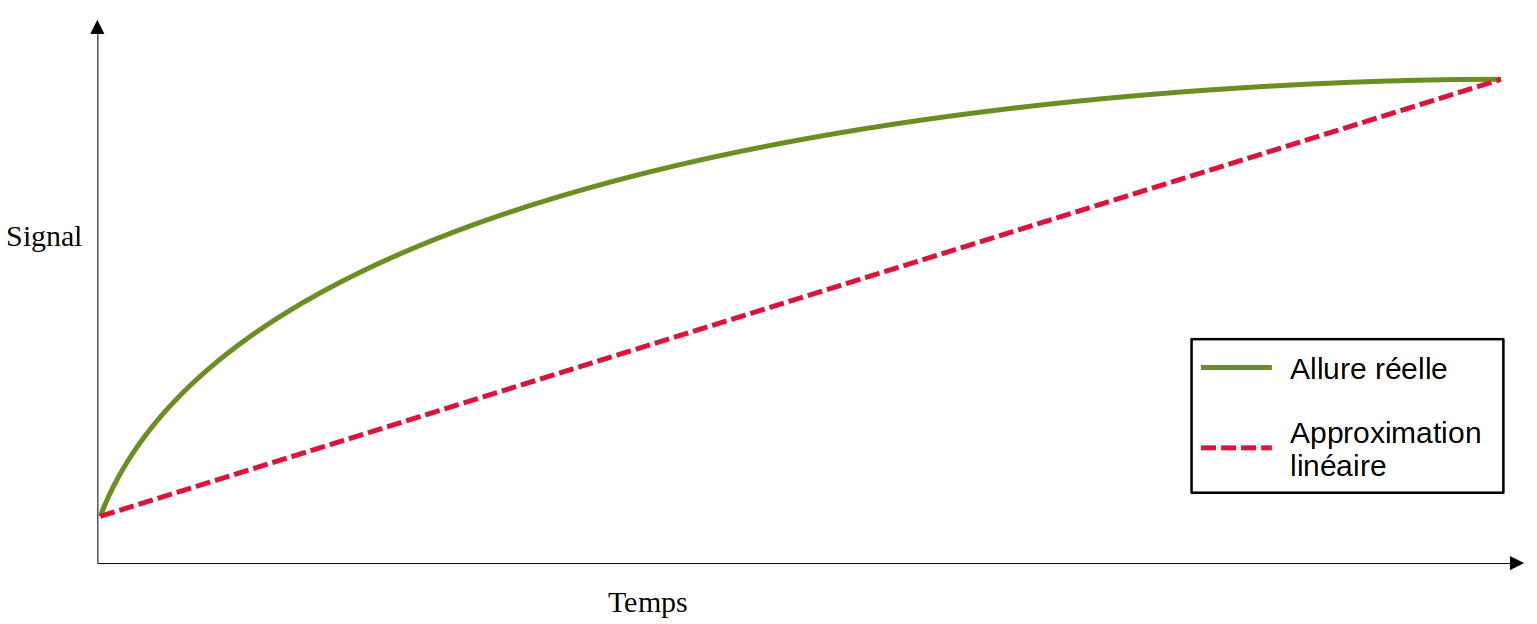
\includegraphics[width=\textwidth]{Images/Base_Vrai_Evol.png}  
        \caption{Allure de la variation théorique de la dérive de l'appareil au démarrage.}
    \end{figure}

    En réalité, le plus grand décalage est dû à un redémarrage de l'appareil. Dans ce cas, il faut attendre plusieurs minutes avant qu'il se stabilise, en suivant un évolution quadratique. On le remarque facilement sur l'inphase du jeu à parcelles carrées (\ref{2_detec_front_ex_in}). L'hypothèse \textbf{(4)} est donc imparfaite, mais plus simple à mettre en œuvre.

    Avec les hypothèse \textbf{(2)} et \textbf{(3)}, on va considérer que le numéro de chaque profil/base peut servir de marqueur temporel ; on peut donc tracer l'évolution des médianes. Pour faciliter la lecture, on prend une échelle de proportionalité car on ne s'intéresse qu'au rapport entre les médianes et non à leur valeur en brut.

\subsubsection{Ajustement des données par base (proportion)}

    \begin{figure}[ht!]
        \centering
        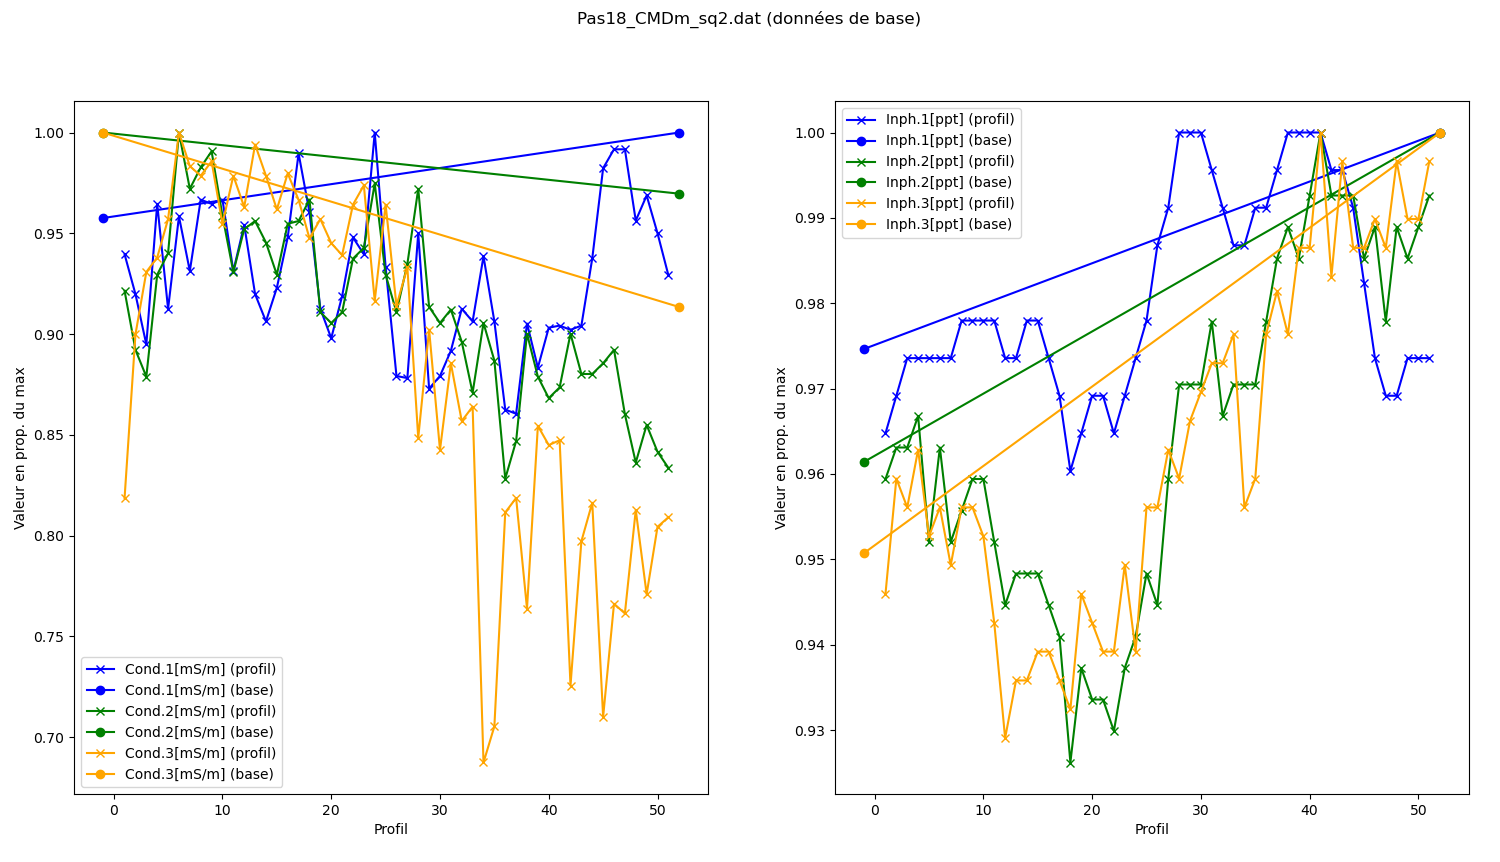
\includegraphics[width=\textwidth]{Images/Base_Avant_sq2.png}  
        \caption{Médiane des bases et profils en fonction de leur ordre chronologique.}
    \end{figure}

    En prenant un jeu avec seulement une base au début et à la fin, on se rend compte que l'évolution globale (décroissante pour \texttt{Cond.}, croissante pour \texttt{Inph.}) semble être suivie à la fois par les profils et par les bases. Selon l'hypothèse \textbf{(1)}, la différence de base témoigne d'un décalage de l'appareil, décalage intervenant donc également sur les profils. On peut donc estimer qu'au moins une partie de cette évolution provient d'une erreur matérielle, celle qu'on cherche à compenser.

    Pour cela on va rabattre la valeur de la base n+1 (à droite) sur celle de la base n (à gauche, en entraînant les profils situés entre de manière linéaire.

    \begin{figure}[ht!]
        \centering
        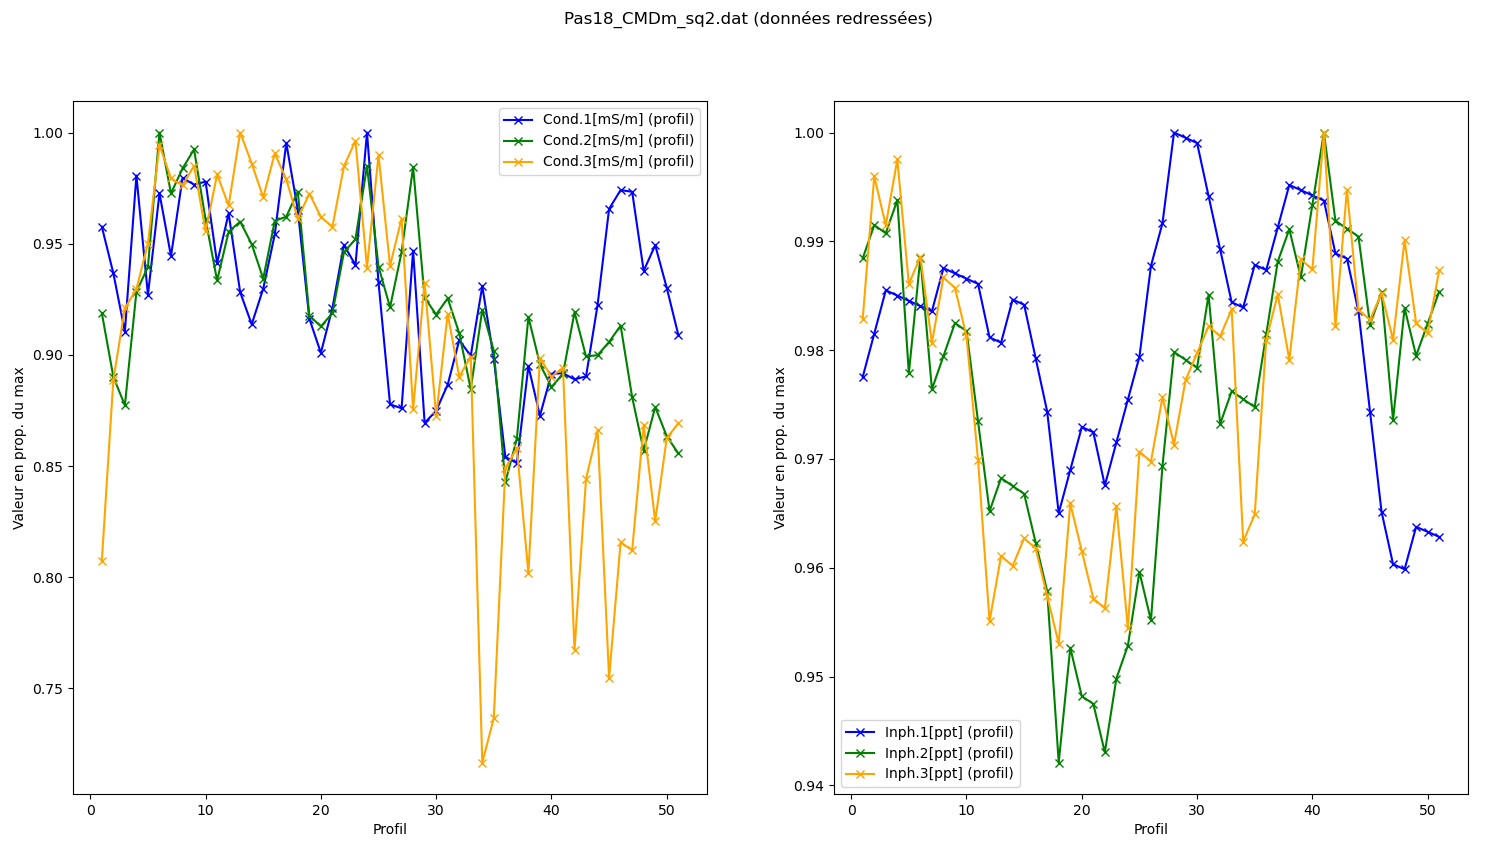
\includegraphics[width=\textwidth]{Images/Base_Apres_sq2.png}  
        \caption{Médiane des profils après ajustement.}
        \label{fig:2_evol_base_im}
    \end{figure}

    Suite à cette opération (figure \ref{fig:2_evol_base_im}), on remarque que la tendance en \texttt{Cond.} est conservée, bien qu'atténuée. Il est donc fort probable que cela viennent du terrain et soit représentatif du secteur. En revanche, \texttt{Inph.} suit désormais une évolution en N inversé, et reste plutôt stable aux extrémités. En s'en fiant aux bases, la tendance croissante était une déformation des mesures.

    \label{2_evol_base_ex_out} En suivant la même méthode, on peut extrapoler cet ajustement avec des jeux possédant des bases au milieu de la prospection (\ref{2_evol_base_ex_in}).

\newpage
\subsubsection{Ajustement des données par base (différence)}

    Dans la plupart des cas, on va préférer corriger le décalage en faisant la différence entre la base n et n+1. Ce choix est souvent plus proche du décalage du zéro de l'appareil. De cette manière, on ne modifie pas l'écart type du jeu. Le reste de la méthode est équivalente.

    \begin{figure}[ht!]
        \centering
        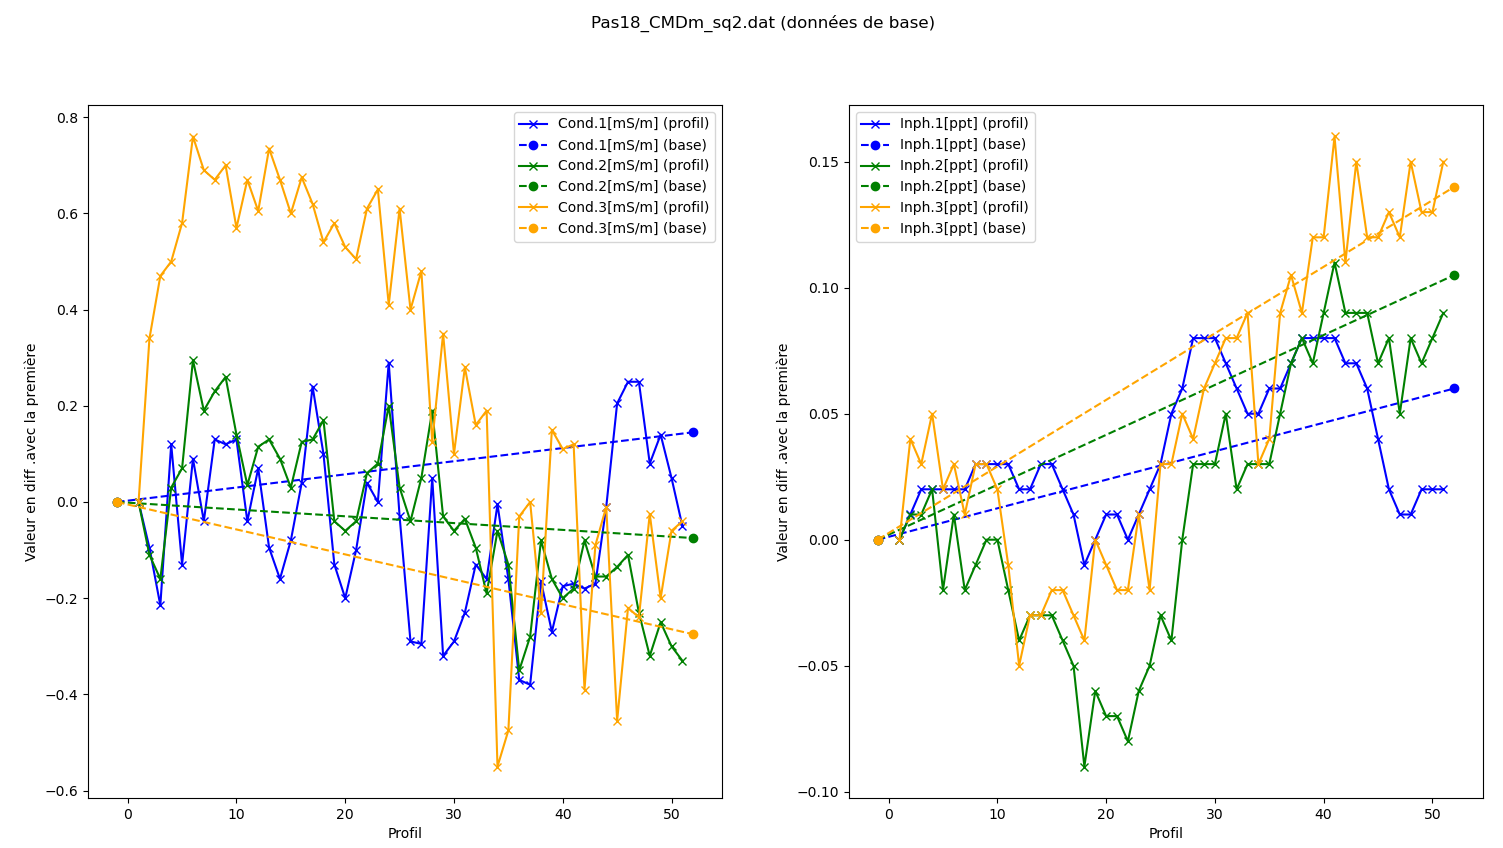
\includegraphics[width=0.8\textwidth]{Images/Base_diff_Avant_sq2.png}  
        \caption{Médiane des bases et profils en fonction de leur ordre chronologique.}
    \end{figure}

    \begin{figure}[ht!]
        \centering
        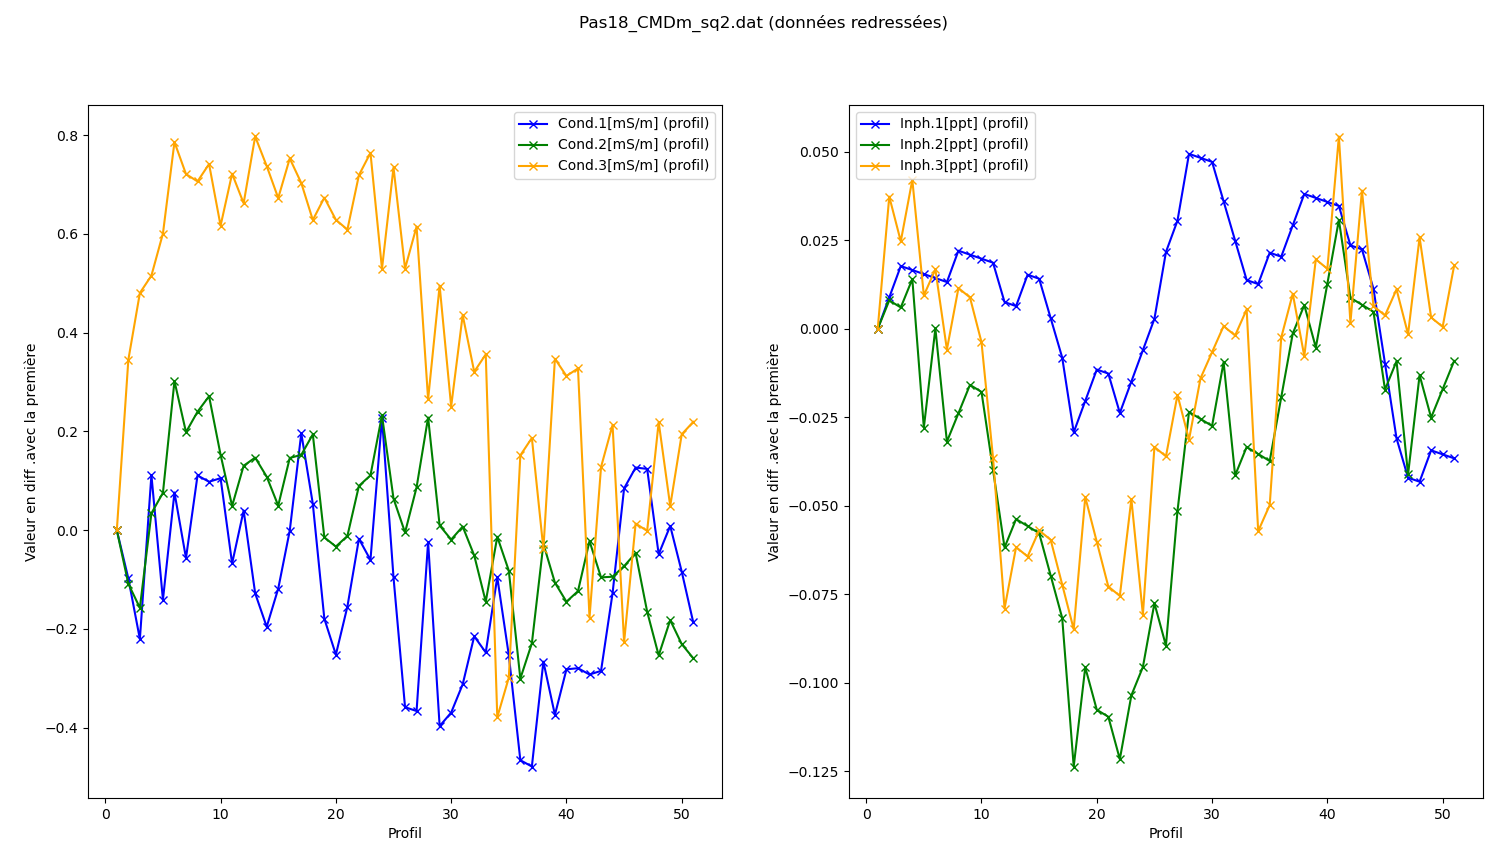
\includegraphics[width=0.8\textwidth]{Images/Base_diff_Apres_sq2.png}  
        \caption{Médiane des profils après ajustement.}
    \end{figure}

    On remarque que les ajustements ont la même allure, mais le référentiel est différent.

\subsubsection{Ajustement manuel}

    Il existe des déformations qui sont visuellement frappantes mais qui ne peuvent pas être traitées par les bases. Par exemple si aucune base n'est prise au milieu de la prospection, il est impossible de détecter le démarrage de l'appareil de cette façon. De plus on doit éviter de chercher à corriger ces déformations automatiquement, car un changement brutal dans les données n'est pas toujours dû à une erreur de l'appareil.

    Pour cela, on peut se servir du graphe des médianes. Si l'utilisateur sait qu'une déformation a eu lieue, il pourra repérer les numéros des profils concernés (en rouge). On appliquera la méthode d'ajustement en prenant les profils précédents et suivant comme "base" (en bleu) pour obtenir les points interpolés (en vert).

    \begin{figure}[ht!]
        \centering
        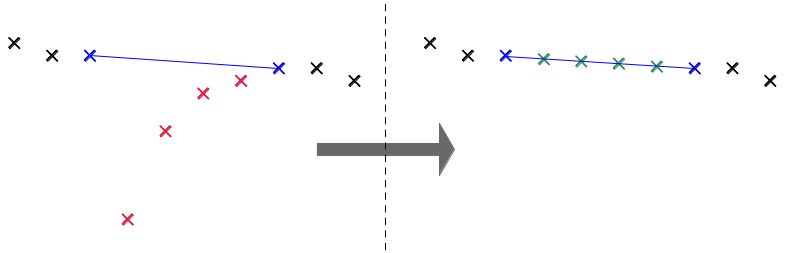
\includegraphics[width=0.8\textwidth]{Images/Base_Schema_of_all_time.png}  
        \caption{Schéma représentatif de la procédure d'ajustement manuel.}
    \end{figure}

    Par exemple, dans le jeu suivant, les failles situées vers le profil 20 et le profil 1 sont le fruit d'une erreur (figure \ref{fig:2_evol_base_man_a}). On cherchera donc à appliquer le correctif uniquement sur ces profils là, pour obtenir la figure \ref{fig:2_evol_base_man_b}. Pour cela, on choisit par exemple la donnée \texttt{Inph.1} sur les profils de 21 à 25. On applique ensuite une regression entre les profils 20 et 26, et on y projette les cinq profils\footnote{Le résultat n'est pas une droite car on arrondit les données à 0.01 près}. On reproduit la procédure autant de fois que nécessaire pour effectuer tous les changements. Si il n'existe pas de profils avant ou après le bloc choisi, on reporte les profils sur un plateau constant donné par la borne connue.
    
    On remarque ensuite que la procédure a bien supprimé (ou du moins atténué) les bandes problématiques sur les figures \ref{fig:2_evol_base_man_c} et \ref{fig:2_evol_base_man_d}.\\

    \begin{figure}[ht!]
        \centering
        \begin{subfigure}[b]{0.475\textwidth}
            \centering
            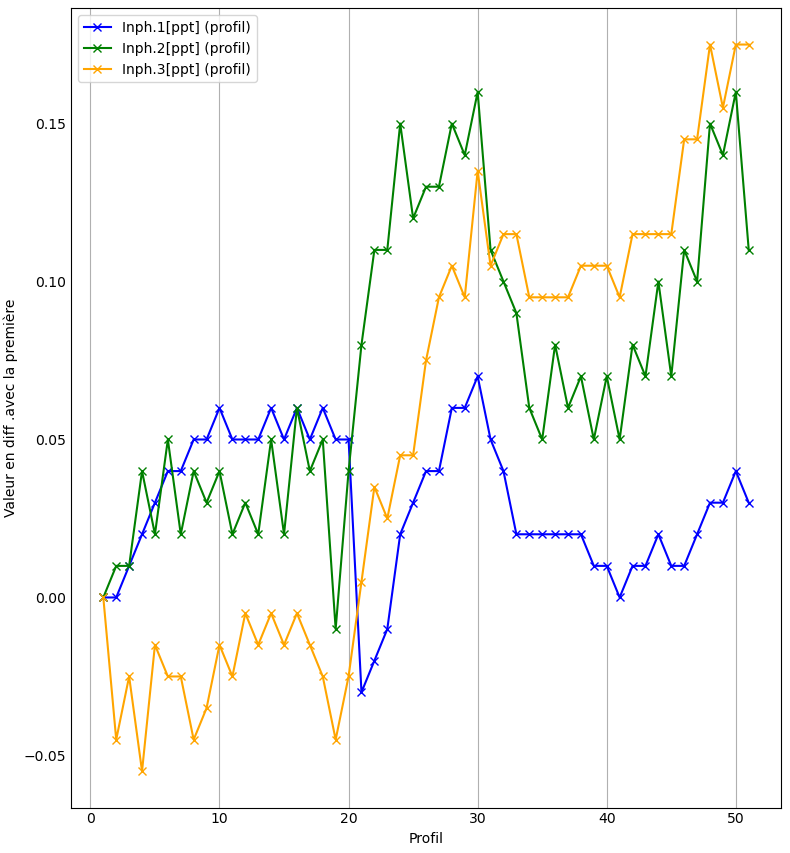
\includegraphics[width=\textwidth]{Images/Base_man_Avant_sq1.png}
            \caption[]%
            {{ \small Évolution des médianes, avant ajustement.}}
            \label{fig:2_evol_base_man_a}
        \end{subfigure}
        \hfill
        \begin{subfigure}[b]{0.475\textwidth}  
            \centering 
            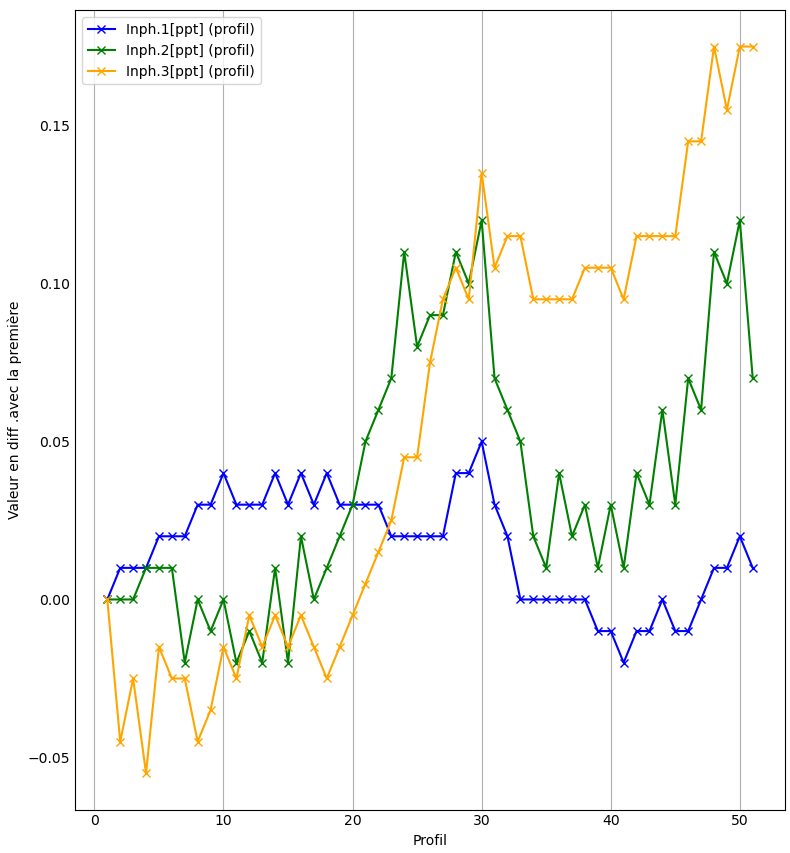
\includegraphics[width=\textwidth]{Images/Base_man_Apres_sq1.png}
            \caption[]%
            {{\small Évolution des médianes, après ajustement.}}
            \label{fig:2_evol_base_man_b}
        \end{subfigure}
        \centering
        \begin{subfigure}[b]{0.475\textwidth}
            \centering
            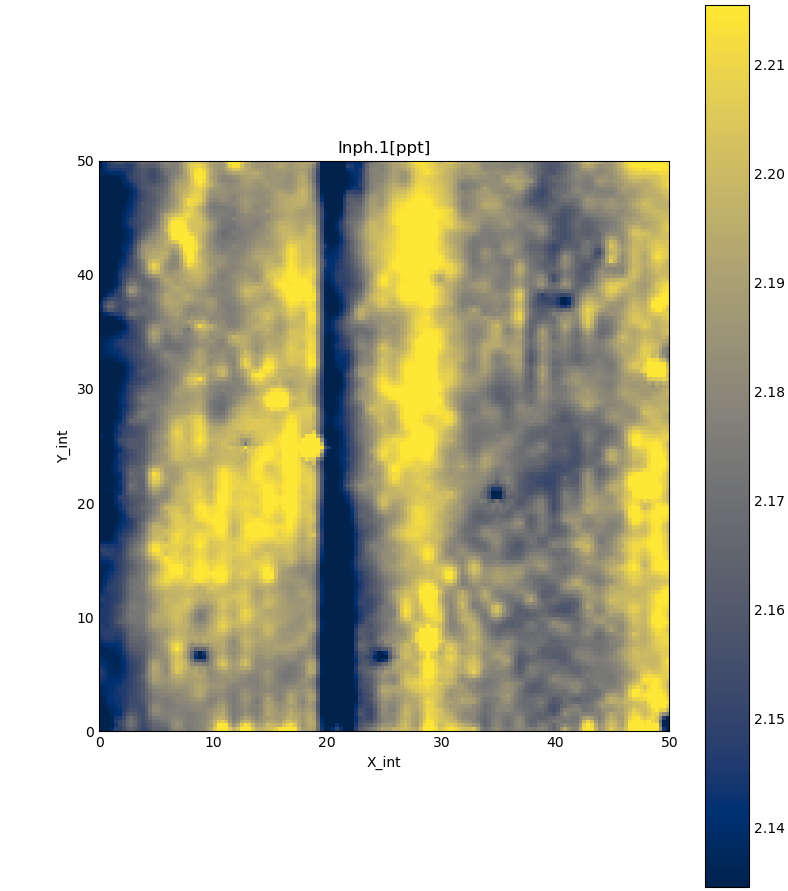
\includegraphics[width=\textwidth]{Images/Base_man_grid_Avant_sq1.png}
            \caption[]%
            {{ \small Affichage du jeu, avant ajustement.}}
            \label{fig:2_evol_base_man_c}
        \end{subfigure}
        \hfill
        \begin{subfigure}[b]{0.475\textwidth}  
            \centering 
            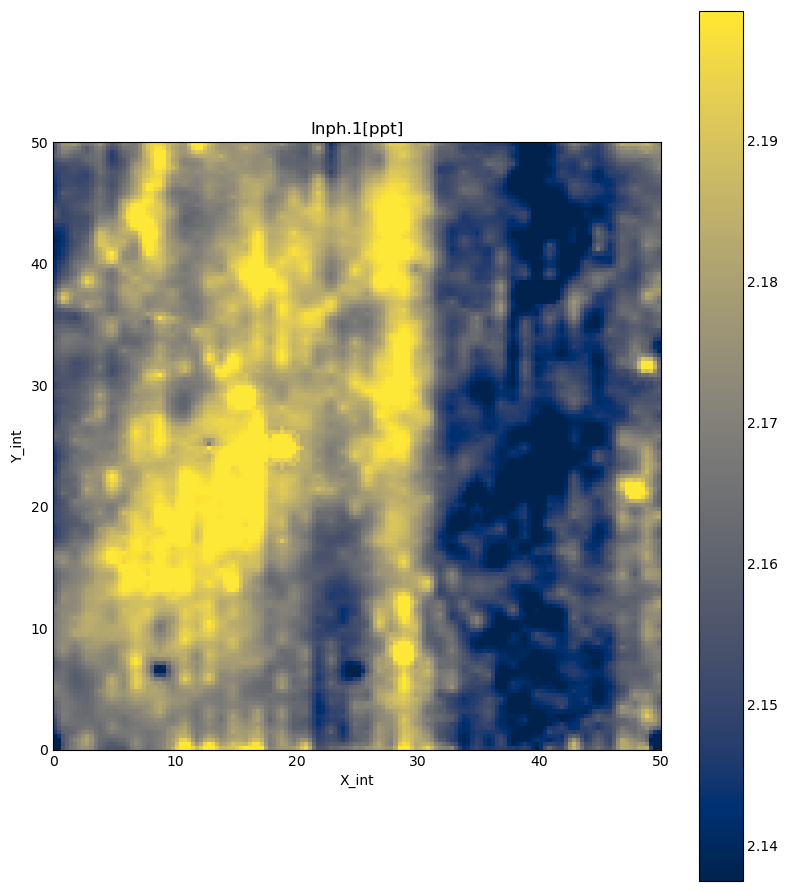
\includegraphics[width=\textwidth]{Images/Base_man_grid_Apres_sq1.png}
            \caption[]%
            {{\small Affichage du jeu, après ajustement.}}
            \label{fig:2_evol_base_man_d}
        \end{subfigure}
        \caption{Intérêt de l'ajustement manuel.}
    \end{figure}
    
    Les deux méthodes (base et manuel) sont complémentaires et utilisent beaucoup de calculs en commun, mais elles ont un but différent. Pour cette raison, on laisse la possibilité de n'en appliquer qu'une des deux si on a un but plus spécifique.

\newpage
\subsection{Affichage en grille}\label{2-3}

    Jusqu'à ici, on s'est intéressé à l'affichage du nuage de point que représente les données, brut ou interpolées. Cependant, pour faciliter la visualisation de la zone, on désire s'affranchir des points et se concentrer sur un découpage en grille. Chaque case de cette grille représente un intervalle de position, et sa couleur doit être représentative des points se trouvant à l'intérieur.

    On se place dans l'ensemble des contraintes suivantes :
    \begin{enumerate}
        \item[\textbf{(1)}] La méthode doit tenir compte de tous les points de l'ensemble, ou au minimum de la répartition globale du nuage de points.
        \item[\textbf{(2)}] La valeur de chaque case doit être cohérente avec celles de ses points, et non simplement un indice de variation quelconque. Par exemple, égale à la moyenne des mesures à l'intérieur.
        \item[\textbf{(3)}] Les cases en périphérie ne contenant aucun point ne doivent pas être colorées. On évitera alors d'évaluer des territoires hors de la prospection.
        \item[\textbf{(4)}] Le temps de calcul (et donc la complexité) doit être suffisament petit pour être applicable à tout jeu de données, sans craindre de crash ou de bloquer pendant des heures.
    \end{enumerate}

    Le méthode suggérée initialement est le \href{https://www.publichealth.columbia.edu/research/population-health-methods/kriging-interpolation#:~:text=Kriging%20is%20one%20of%20several,over%20a%20continuous%20spatial%20field.}{kriging}. C'est une technique statistique permettant grâce à un variogramme de projeter des données sur une grille de manière continue. La méthode de diffusion dépend du variogramme (gaussien, exponentiel, linéaire, sphérique...). Chaque point influence les cases autour, avec une intensité proportionnelle à leur distance.

    Il existe plusieurs librairies Python effectuant le krigeage, comme par exemple \href{https://gstlearn.org/}{gstlearn}. Malheureusement, il y a de nombreux problèmes avec cette application :

    \begin{enumerate}
        \item[$\bullet$] La librairie n'est qu'assez mal documentée car moins utilisée que d'autres librairies scientifiques, la plupart des informations provenant du \href{https://soft.mines-paristech.fr/gstlearn/courses-latest/python/}{site mines-paristech} notamment de \href{https://soft.mines-paristech.fr/gstlearn/doxygen-latest/}{la documentation officielle en C++} (heureusement équivalente à Python). Il est difficile de trouver la procédure que l'on recherche vraiment.
        \item[$\bullet$] Beaucoup de fonctionalités sont fortement adaptées voire réservées à un type de fichier qui leur est spécifique : le NeutralFile (.NF). Pratiquement tous leurs exemples tournent autour d'ailleurs. Cependant, les seuls semblant exister sont ceux donnés en exemple de la librairie ; et il n'existe pas de moyen d'en créer soi même\footnote{"A last solution is to import it directly from the set of demonstration files (provided together with the package and called fileNF) and stored in a specific format (Neutral file). These NF (or neutral file) are currently used for serialization of the gstlearn objects. They will probably be replaced in the future by a facility backuping the whole workspace in one step." (\href{https://soft.mines-paristech.fr/gstlearn/1.3.1/courses/r/02_Db.html}{source}) } Parmi les fonctionalités bloquées, on trouve la restriction de la grille aux points de l'ensemble. Il semble donc peu probable de répondre à l'exigence [3] automatiquement.
        \item[$\bullet$] La complexité de l'algorithme semble être fortement quadratique. Peu importe le variogramme utilisé il est long voire impossible avec mon ordinateur de dépasser plusieurs milliers de points, malgré une grille réduite.
    \end{enumerate}

    Cela ne signifie pas que le krigeage n'est pas applicable en l'état, mais seulement que des étapes supplémentaires doivent être trouvées.

\subsubsection{Découpage de la grille}

    Afin de préparer la grille d'interpolation, on définit une fonction effectuant les tâches suivantes :

    \begin{enumerate}
        \item[$\bullet$] Attribuer une valeur à chaque case en fonction des points s'y trouvant. Si la case est vide, on lui attribue la valeur spécifique $NaN$. Sinon, on indique la présence d'un point par un $0$.
        \item[$\bullet$] On ajuste le résultat trouvé en fonction des cases avoisinantes. Pour cela, on se sert d'un rayon \texttt{radius} où chaque case à l'intérieur du cercle est pondérée par un coefficient dérivé de sa distance au centre. On introduit un seuil \texttt{seuil}, servant à définir si une case précédemment vide doit être ajoutée quand même ; sinon on la laisse vide.
    \end{enumerate}

    Cette procédure permet de déterminer quelles sont les cases à exclure de l'interpolation, et donc répondre à l'exigeance \textbf{(3)}. Sa complexité est en $O(n)$ sur les données, $O(n^{2})$ sur la précision de la grille, $O(n^{2})$ sur le rayon (ce qui est optimal au vu des conditions). Le temps de calcul est raisonnable dans la majorité des cas, en général moins de dix secondes (exigeance \textbf{(4)}).

    La répartition des coefficients dépend d'une fonction polynomiale, où le paramètre \texttt{seuil} détermine la vitesse de décroissance (le degré du terme).

    Ainsi, plus le \texttt{seuil} est grand, plus on donne d'importance aux points très proche. Si \texttt{seuil} $= 0$ par exemple, on obtient une grille à coefficients constants. Il est aussi possible de considérer des \texttt{seuil}s négatifs, dans ce cas on prendra le cas \texttt{seuil} $= 0$ multiplié par $1 -$ \texttt{seuil} (pour ne pas créer d'incohérences). En l'occurence, on préférera des \texttt{seuil}s faibles (càd proches de 0) pour boucher les trous, car les cases à l'intérieur sont souvent à proximité de beaucoup de cases sans être nécessairement à 1 de distance. Cependant, si le jeu ne crée pas de trous, un fort \texttt{seuil} permet de découper plus violamment la frontière.

    \begin{figure}[ht!]
        \centering
        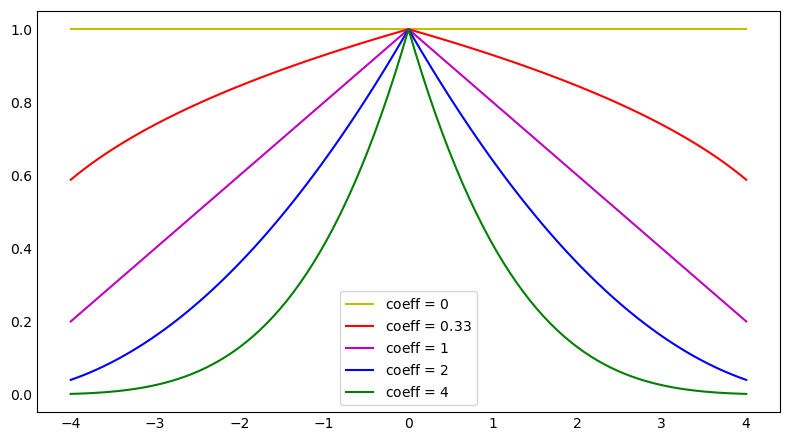
\includegraphics[width=0.8\textwidth]{Images/Grid_FirstAlg_CoeffCurve.png}
        \caption{Exemples de répartition des coefficients en fonction de la distance au centre.}
    \end{figure}

    \label{2_grid_firstalg_coeff_out} On peut ensuite appliquer cette loi 1D sur une grille 2D (\ref{2_grid_firstalg_coeff_in}).

\subsubsection{Heatmap}

    Afin de faciliter le choix du \texttt{seuil}, on propose de passer par une heatmap de densité de case. On affiche deux représentations :

    \begin{enumerate}
        \item[$\bullet$] À gauche, la heatmap attribuant un score de densité à chaque case.
        \item[$\bullet$] À droite, le découpage induit, où on ne prend que les cases avec 1 de score ou plus. On représente également les points de l'ensemble initial pour pouvoir juger de la pertinence du découpage.
    \end{enumerate}

    \begin{figure}[ht!]
        \centering
        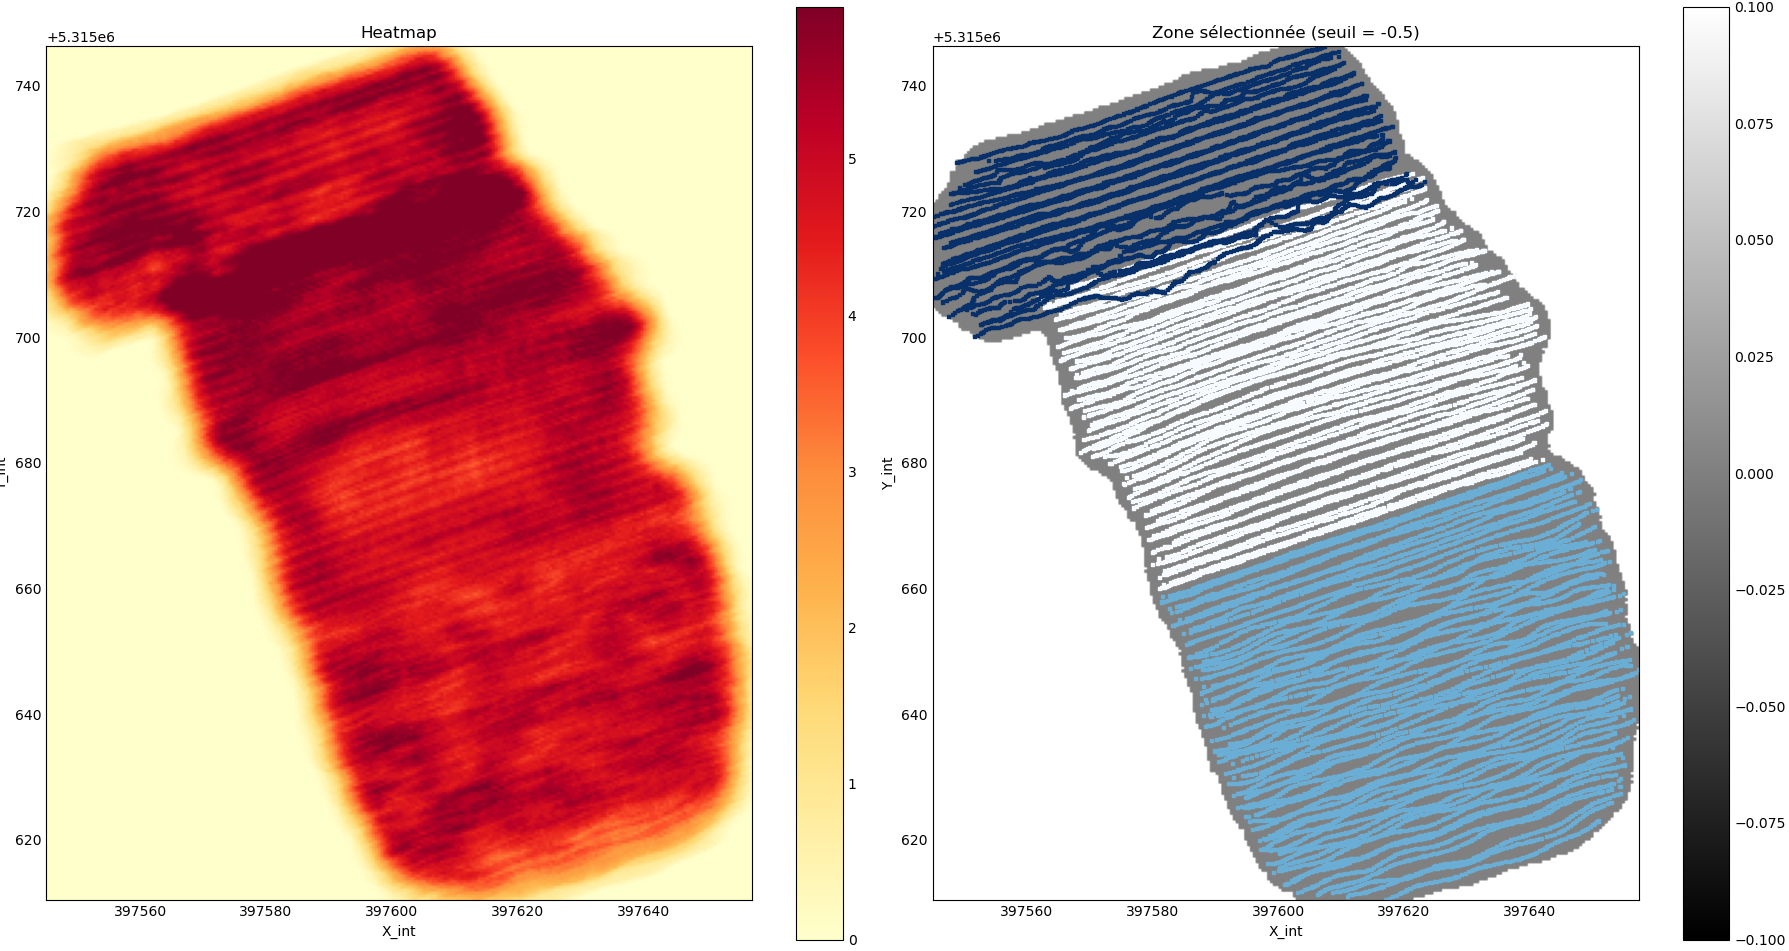
\includegraphics[width=\textwidth]{Images/Grid_Heatmap_p300.png}
        \caption{Heatmap et découpage, [\texttt{prec} = 300].}
    \end{figure}
    
    En faisant varier le \texttt{seuil}, on peut expérimenter plusieurs découpages, jusqu'à trouver celui qui correspond le mieux au jeu.

    Un fois fini, on pourra lancer une interpolation/krigeage avec le \texttt{seuil} trouvé.

    Il est important de noter que si l'on souhaite réaliser l'interpolation sur plusieurs voies d'une même prospection, on aura des coordonnées différentes. Cependant, la variation est en principe suffisament petite pour ne pas faire différer le découpage de manière significative. On peut alors se contenter d'afficher la heatmap pour le premier couple de position uniquement.

\newpage
\subsubsection{Découpage de la grille 2}

    Une autre solution pour le découpage est de s'intéresser à la direction dans laquelle se situent les points aux alentours. Par exemple, il n'y a pas forcément de différence sur le nombre de points dans l'entourage ou leur distance entre un trou (une zone vide enclavée) et le voisinage d'une frontière. En revanche un point situé dans un trou devrait avoir un voisinage tout autour de lui (à condition que le rayon de la fenêtre les détecte), contrairement à un bord de zone.

    Pour faire la distinction, on va utiliser trois arguments :
    \begin{enumerate}
        \item[\textbf{(1)}] Si le voisinage d'un point comprend moins de deux points, il est retiré (trop excentré).
        \item[\textbf{(2)}] On calcule le vecteur moyen de distance entre le point de la grille et les points du jeu de données dans la fenêtre. Si sa norme est plus grande que la moitié du rayon de la fenêtre, le point de la grille est retiré (points concentrés dans la même zone).
        \item[\textbf{(3)}] On note l'angle orienté formé par le point de la grille et chaque point du voisinage. On calcule ensuite le plus grand écart existant entre deux angles consécutif, c'est-à-dire le plus grand cône sans aucun point. Si celui-ci dépasse 180\textdegree le point de la grille est retiré (trop grande zone vide).
    \end{enumerate}

    Avant d'évaluer le résultat, discutons le choix de ces critères.

    Tout d'abord, le critère \textbf{(1)} concerne des cas déjà exclus par le critère \textbf{(3)}, mais il ne nécessite aucun calcul et permet d'exclure la plupart des cases en périphérie.

    Le critère \textbf{(2)} ne suffit pas forcément à exclure les points très proches de la frontière (ou dans un léger creux), car leur moyenne va être écrasée par leur proximité. Or si on veut être très précis, aucun point ne devrait dépasser du jeu.

    Le critère \textbf{(3)} inclut souvent les cas gérés par le critère \textbf{(2)}, mais il pourrait donner trop d'importance à un point isolé (peu représentatif), cassant un cône vide en deux.

\newpage
    Résultat :

    \begin{figure}[ht!]
        \centering
        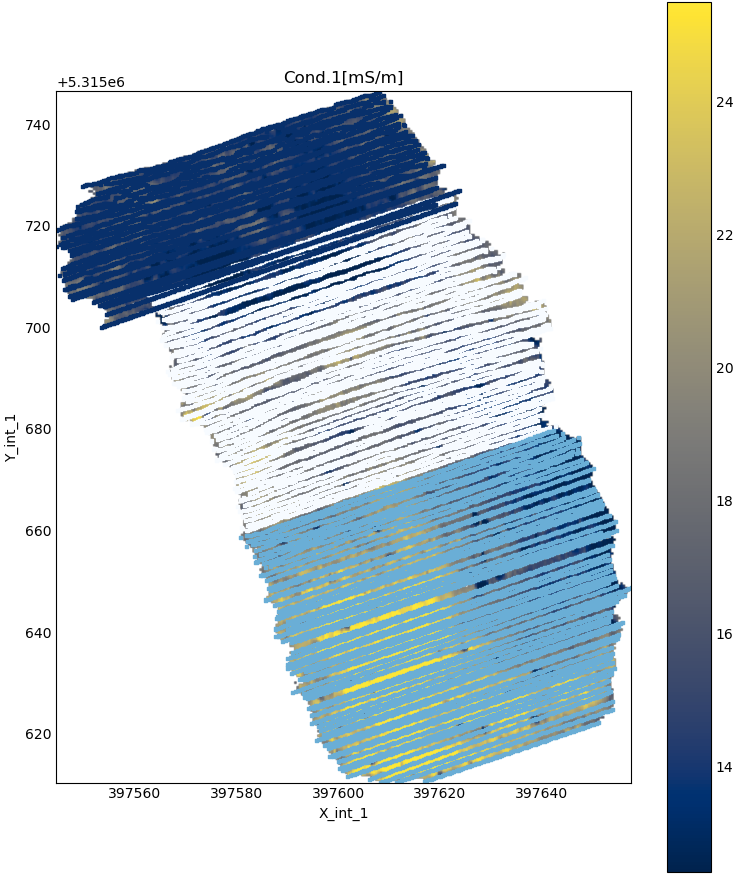
\includegraphics[width=\textwidth]{Images/Grid_SecondAlg_r4p300.png}
        \caption{Interpolation linéaire, [\texttt{prec} = 300, \texttt{radius} = 4].}
    \end{figure}

    Cette méthode rogne beaucoup mieux la frontière, mais a tendance à créer des protubérences dans les creux, car les points au centre détecte le haut et le bas du "U".

    \begin{figure}[ht!]
        \centering
        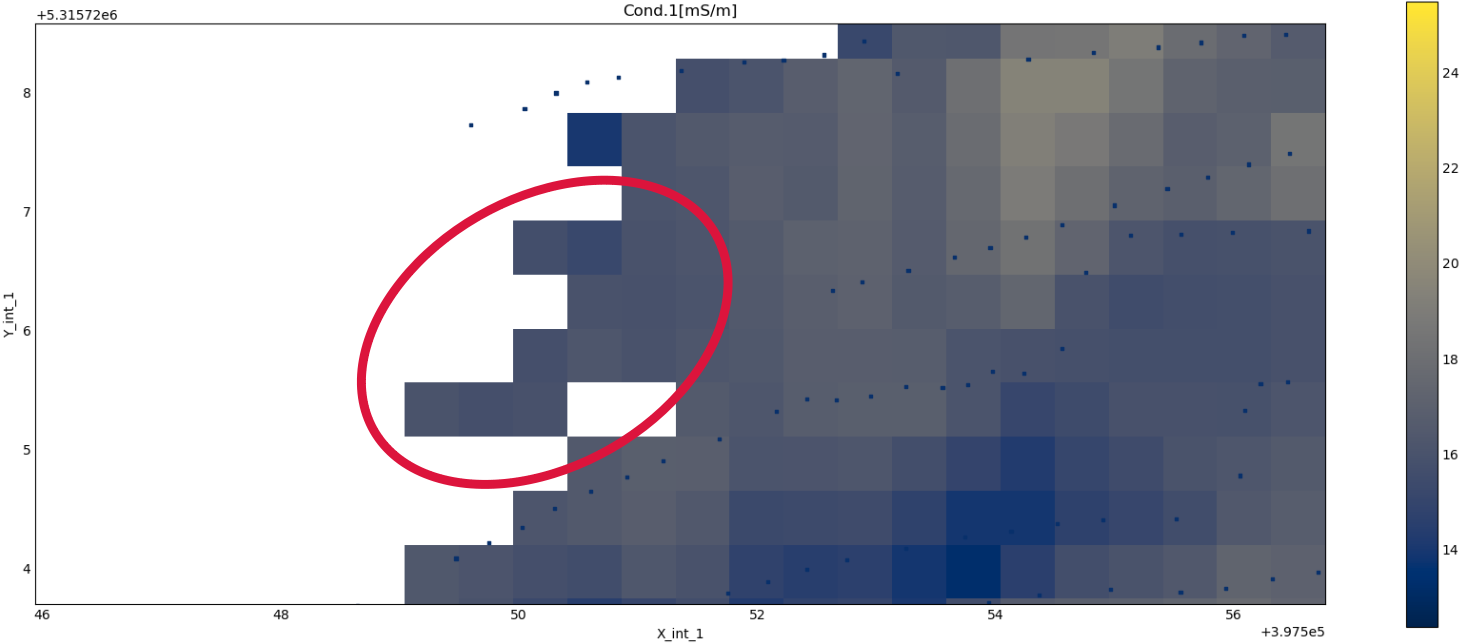
\includegraphics[width=\textwidth]{Images/Grid_SecondAlg_Hallucination.png}
        \caption{Bande sans point de données conservée.}
    \end{figure}

\newpage
\subsubsection{Interpolation classique}

    La solution la plus simple pour mettre en grille des données est de passer par un algorithme d'interpolation, comme fourni par la bibliothèque \href{https://docs.scipy.org/doc/scipy/reference/generated/scipy.interpolate.griddata.html}{scipy}. La fonction \texttt{griddata} propose trois types d'interpolateur : \texttt{nearest} (neighbor), \texttt{linear} et \texttt{cubic}. Leur utilisation est très rapide.

    \begin{figure}[ht!]
        \centering
        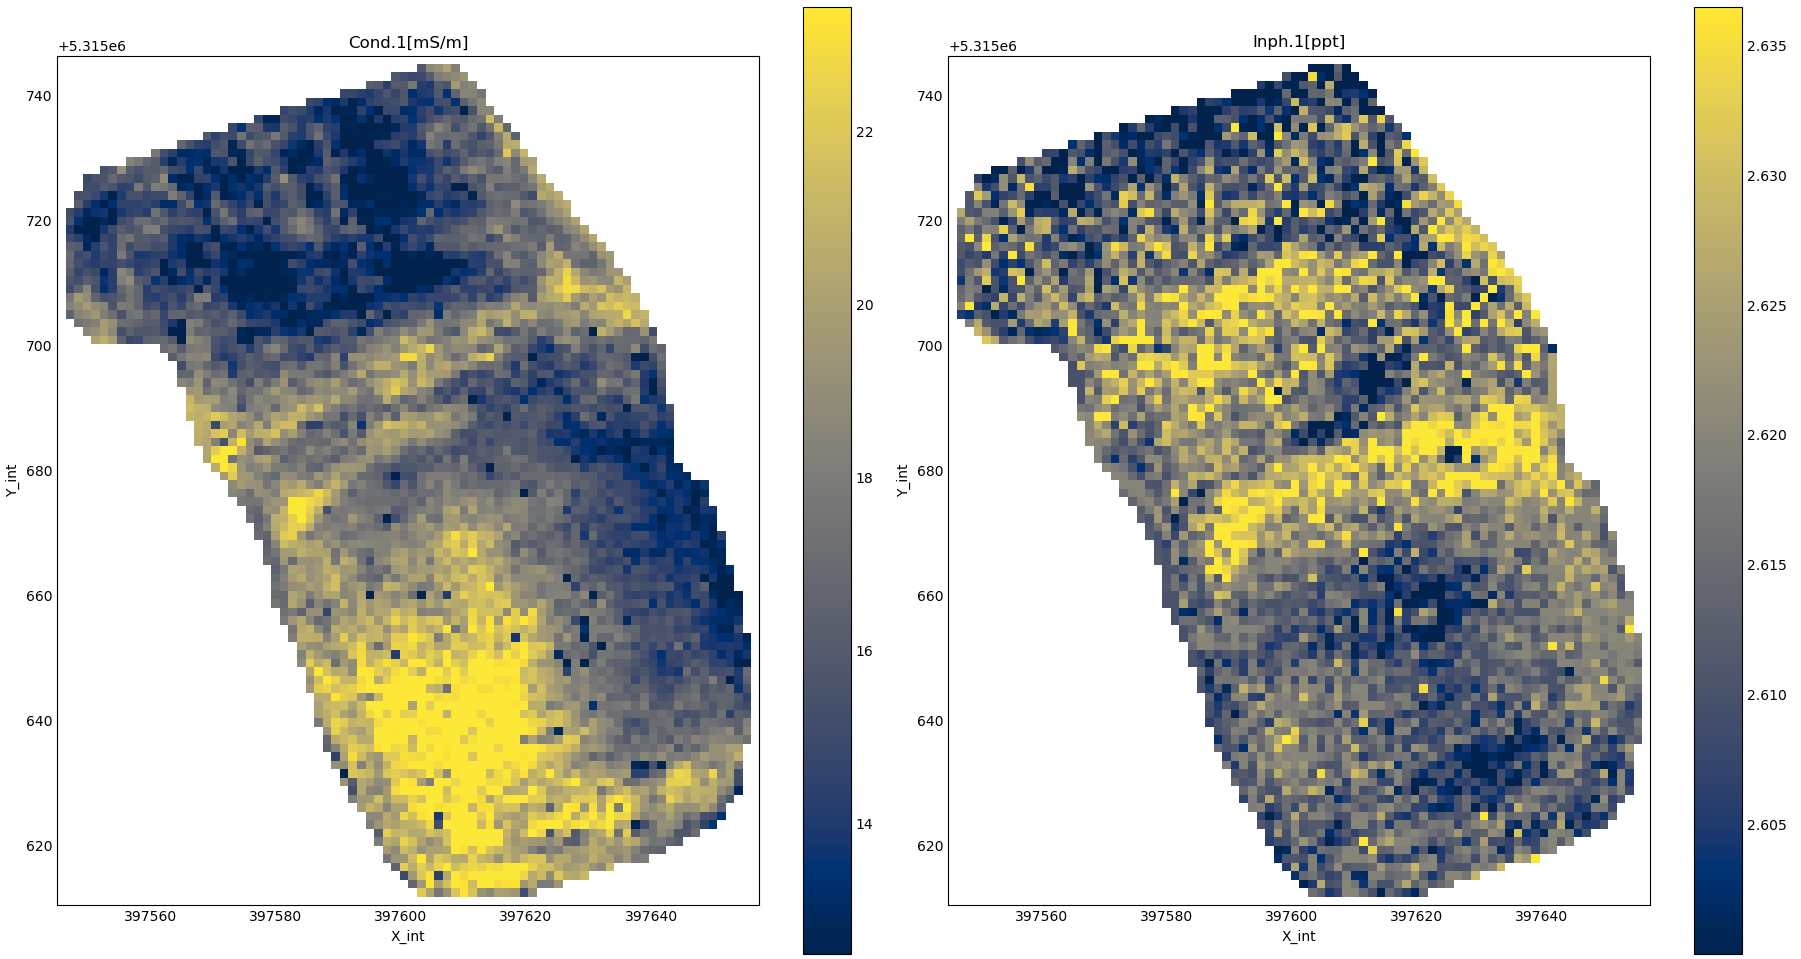
\includegraphics[width=0.8\textwidth]{Images/Grid_Interplin_r1c1p100.png}
        \caption{Interpolation linéaire, [\texttt{prec} = 100].}
    \end{figure}

    Il est important de noter que \texttt{scipy} possède automatiquement une option pour découper l'ensemble, mais elle ne le fait que de manière convexe. On crée donc de l'erreur.

    \begin{figure}[ht!]
        \centering
        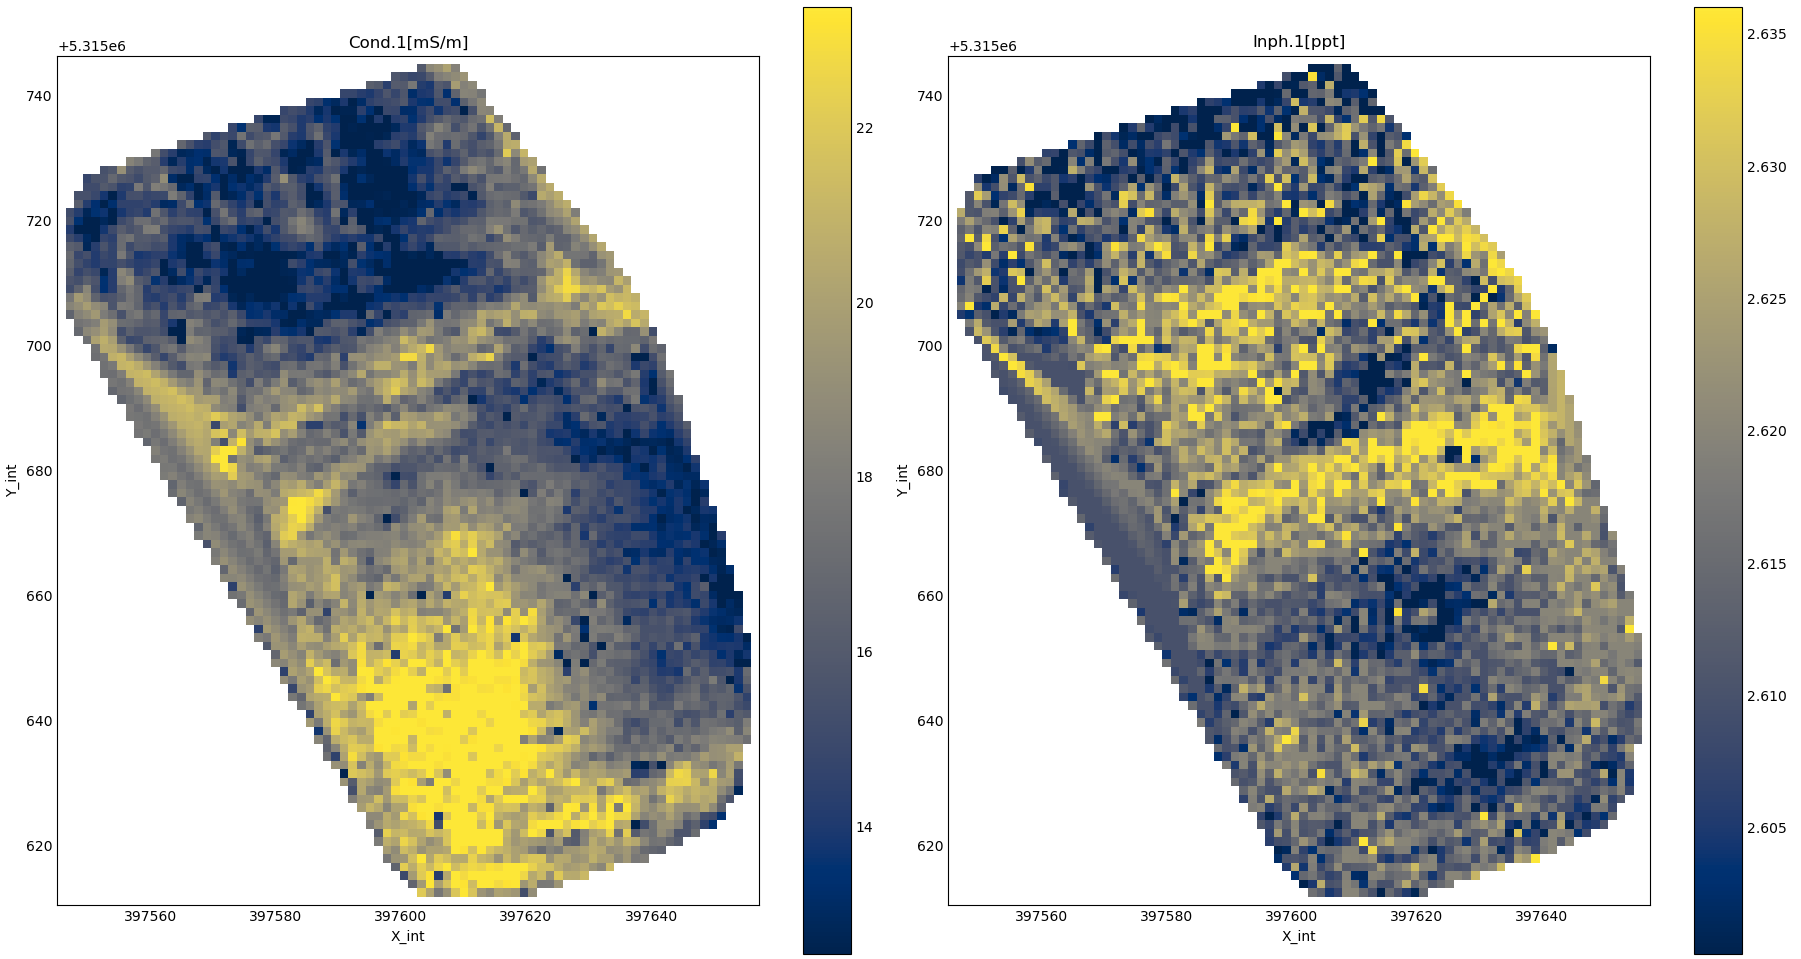
\includegraphics[width=0.8\textwidth]{Images/Grid_Interplin_r1c1p100_nocrop.png}
        \caption{Interpolation linéaire avec découpage convexe, [\texttt{prec} = 100].}
    \end{figure}

\subsubsection{Krigeage}

    On peut appliquer le kriging sur une grille vierge. On obtient alors une grille entièrement remplie comme celle ci (\ref{fig:2_grid_krex_im}):

    \begin{figure}[ht!]
        \centering
        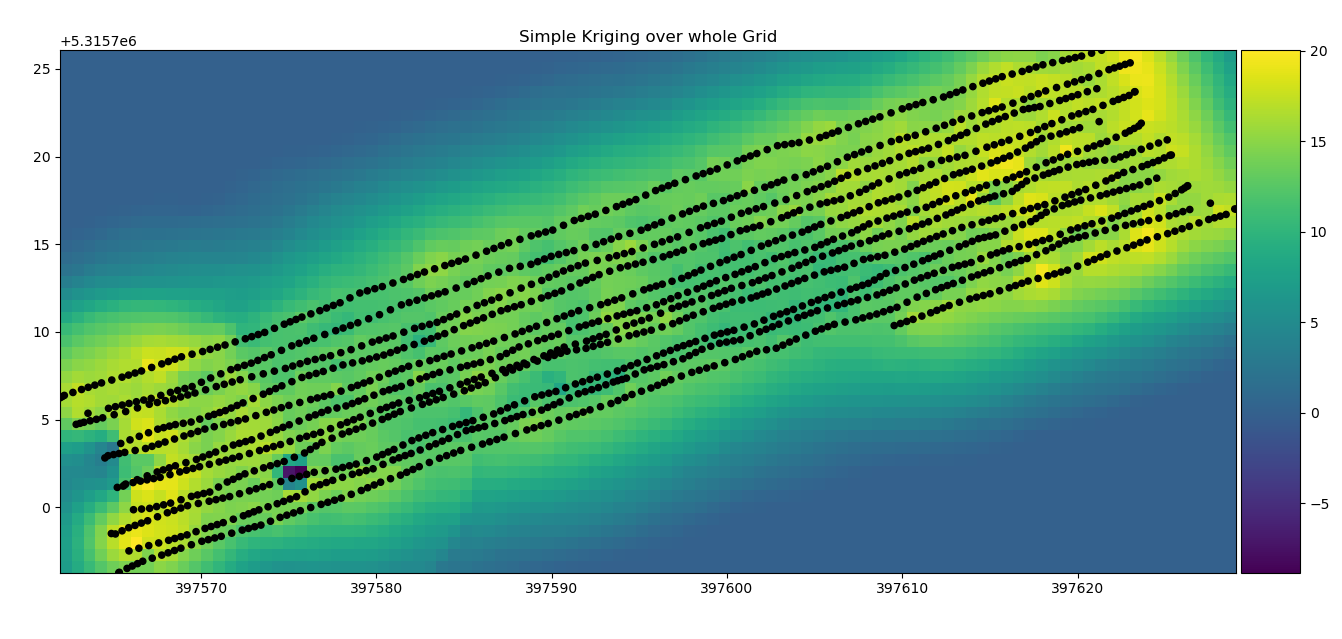
\includegraphics[width=0.8\textwidth]{Images/Grid_Kriging_ex.png}
        \caption{Exemple de kriging sur une section de 1000 points.}
        \label{fig:2_grid_krex_im}
    \end{figure}

    Il suffit alors de supprimer les bordures à l'aide de la grille de la premières étape pour obtenir le kriging restreint à l'ensemble de points.
    
    Cependant, le résultat (c'est-à-dire la valeur obtenue sur chaque case) dépend du choix du variogramme (\ref{fig:2_grid_kriging_variog}). Si il n'est pas adapté, le kriging ne rendra pas compte de l'ensemble correctement. D'abord, on choisit la manière de calculer le variogramme expérimental (nombre de directions, angle, distance, nombre d'intervalles). Pour chaque direction, on obtient à l'aide de covariances la correlation entre les points selon leur distance. Plus la valeur du variogramme est faible, plus il y a corrélation. Grâce à son allure on peut en déduire le modèle statistique qui l'approxime le mieux. Plus le modèle (en trait plein) se rapproche du variogramme expérimental (en pointillés), plus il sera efficace pour estimer la grille.

     \begin{figure}[ht!]
        \centering
        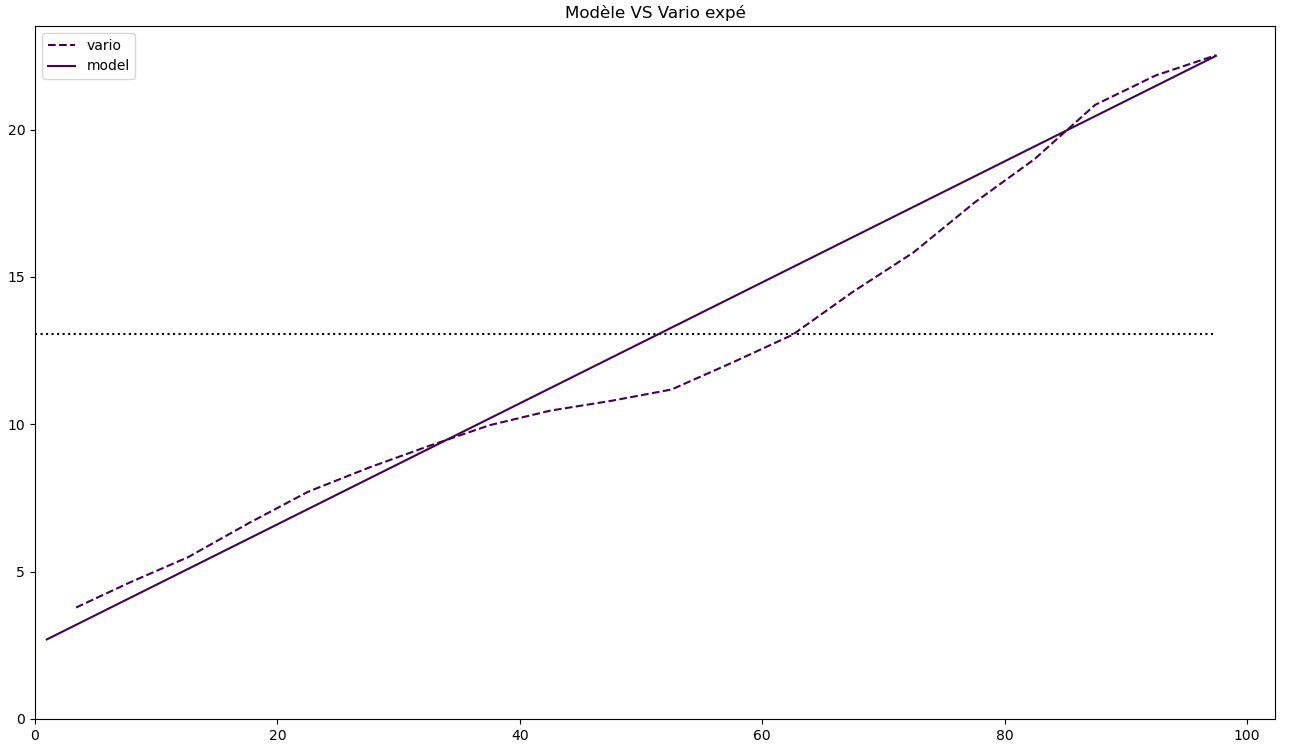
\includegraphics[width=0.6\textwidth]{Images/Grid_Kriging_Variog.png}  
        \caption{Variogramme expérimental VS Modèle.}
        \label{fig:2_grid_kriging_variog}
    \end{figure}

    Pour cela, on laisse à l'utilisateur le choix de la combinaison de modèles du variogramme, parmi ceux disponibles dans la librairie (gaussien, sphérique, exponentiel...).

    Sur l'exemple ci-dessus, on a utilisé un nugget effect couplé à un modèle linéaire.

    On constate facilement l'importance du choix lorsque celui-ci est mauvais. Dans ce cas, il n'est plus possible de correctement interpréter la prospection (\ref{fig:2_grid_kriging_im}).

    \begin{figure}[ht!]
        \centering
        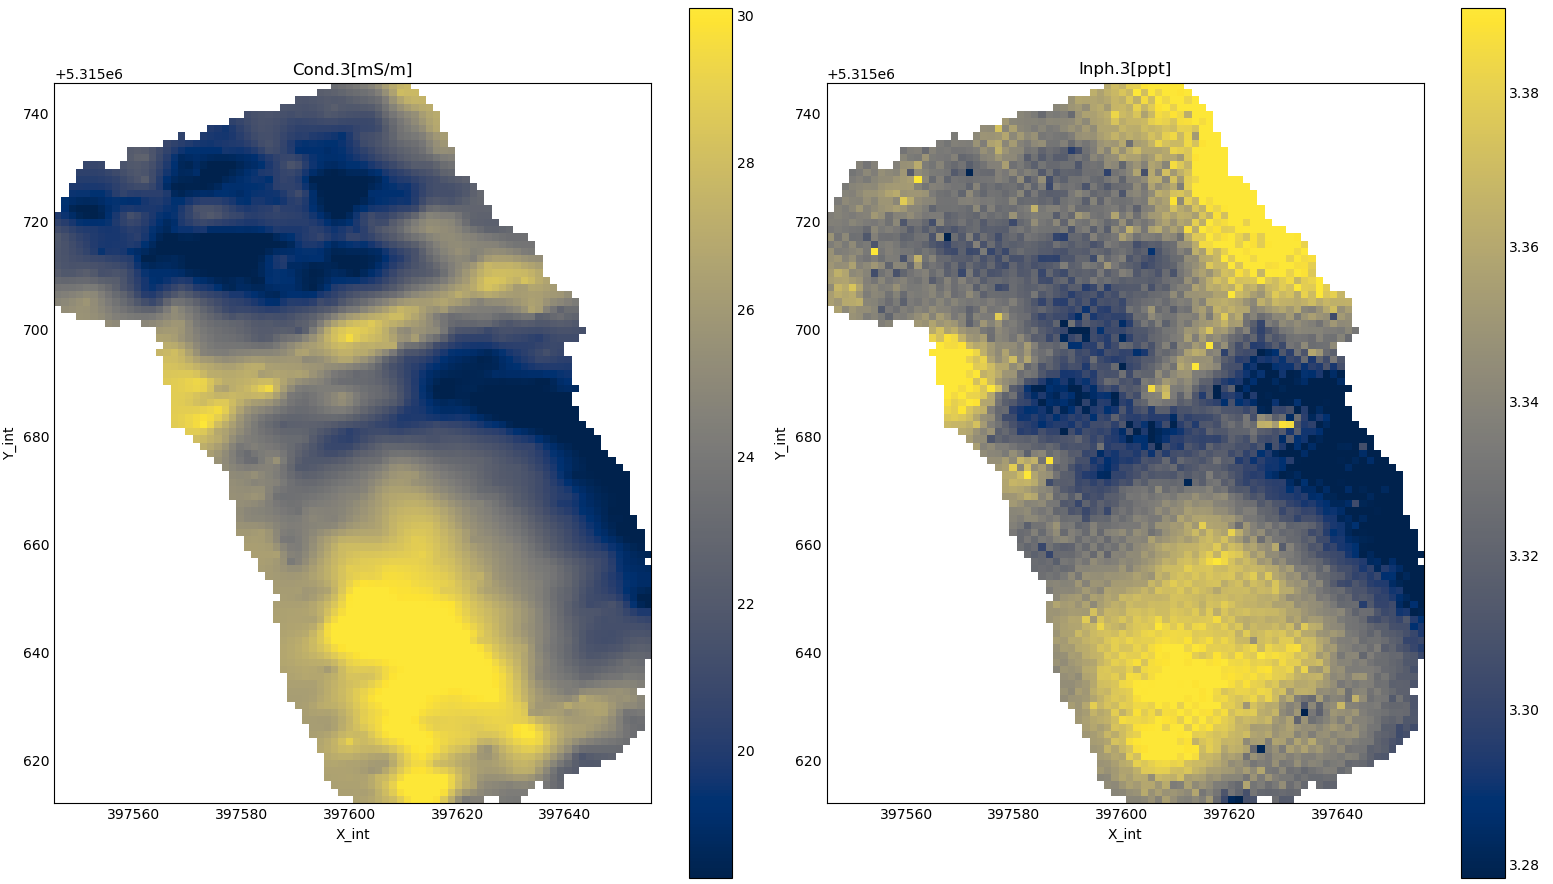
\includegraphics[width=0.8\textwidth]{Images/Grid_Kriging_r4c04p100_3.png}  
        \caption{Grille après kriging [\texttt{prec} = 100], réussi.}
        \label{fig:2_grid_kriging_im}
    \end{figure}

    \begin{figure}[ht!]
        \centering
        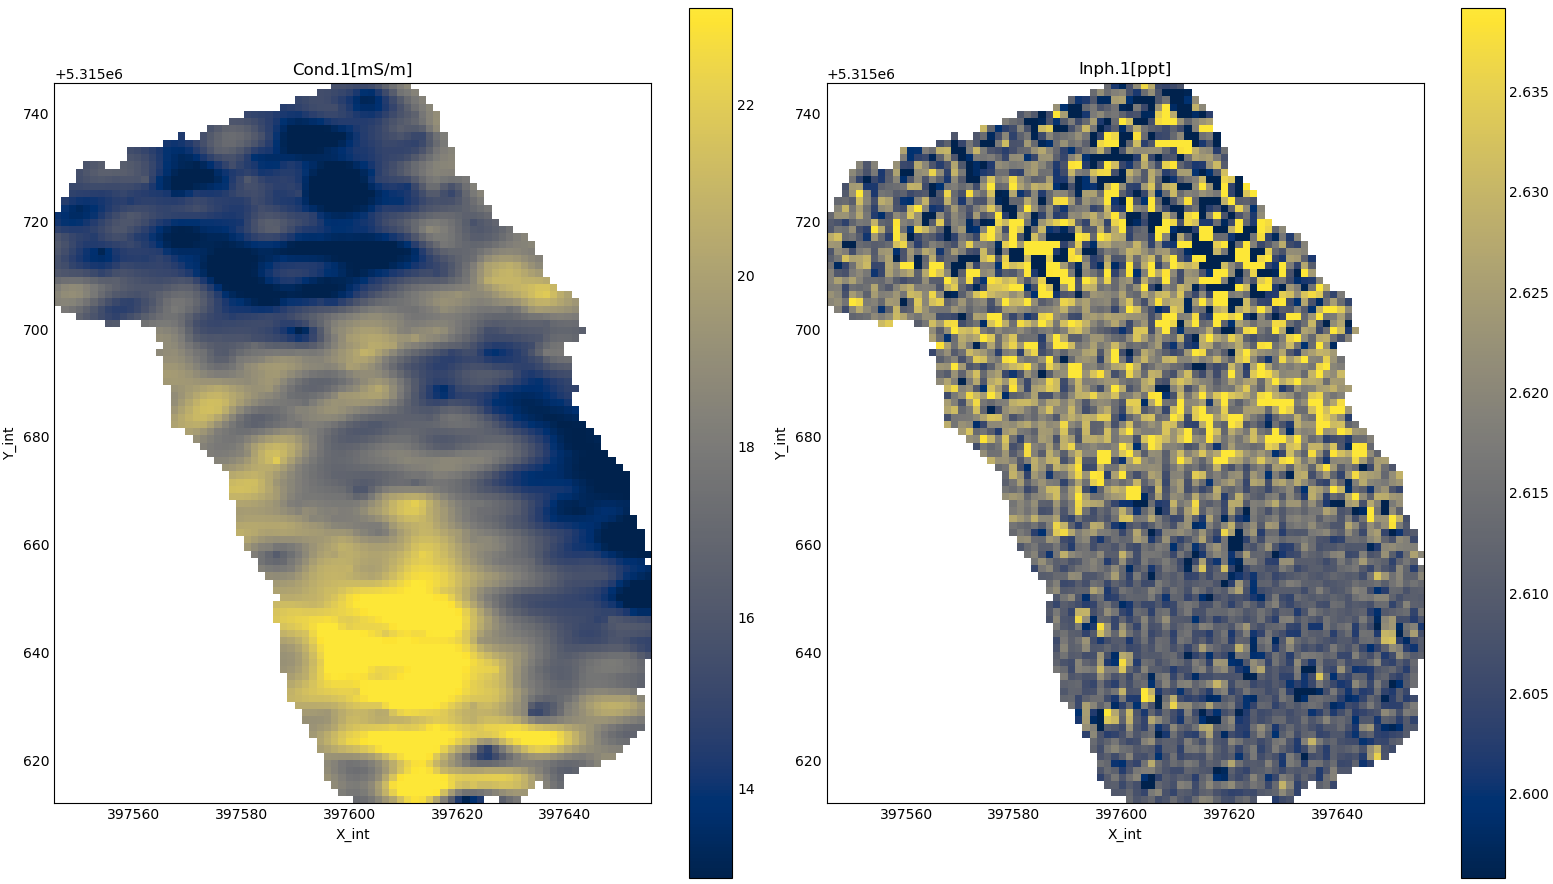
\includegraphics[width=0.8\textwidth]{Images/Grid_Kriging_r4c04p100.png}  
        \caption{Grille après kriging [\texttt{prec} = 100], raté.}
    \end{figure}

    Pour résumer, il peut être intéressant de se contenter de l'interpolation simple pour la visualisation, car elle possède de bien meilleurs performances en temps. Il est d'ailleurs préférable d'expérimenter le découpage parfait avant de passer au krigeage gràce à la heatmap, au risque de perdre un résultat sur la restriction de grille. De plus, son utilisation ne nécessite pas d'établir un variogramme cohérent, ce qui n'est pas trivial. Cependant, les techniques de diffusion sont constantes et ne s'adaptent pas au jeu.

    Le krigeage est intéressant lorsque le jeu ne possède qu'un faible nombre de points espacés, avec donc beaucoup de cases inconnues. Il permet de mieux diffuser la répartition de couleurs en gommant les valeurs extrêmes (points singuliers à valeur extrême). Sa forte necessité en calcul ne permet pas d'application sur des jeux denses (sauf en temps très long). C'est pourquoi on prendra automatiquement que 1000 points au maximum, répartis sur l'ensemble de sorte à conserver l'exigeance \textbf{(1)}. On pourra cependant forcer l'opération sur le jeu complet. De plus, le variogramme permet de répondre à des cas spécifiques où considérer des points éloignés peut être intéressant (par exemple si des couches homogènes de matériaux se répètent). Si on cherche à utiliser les données en grille lors d'un traîtement, le kriging couplé à un bon variogramme permet de minimiser l'erreur de diffusion.

\subsubsection{Format de stockage}

    Contrairement aux autres étapes du traitement, on peut avoir intérêt à conserver la grille sous forme matricielle plutôt que sous forme de dataframe, car elle permet l'affichage par la fonction \href{https://matplotlib.org/stable/api/_as_gen/matplotlib.pyplot.imshow.html}{\texttt{imshow}} (celle en grille). Cependant, si on souhaite utiliser par la suite les données pour d'autres opérations, on aura besoin du dataframe.

    Par conséquent, l'utilisateur doit pouvoir choisir dans lequel des deux formats enregistrer la grille. Pour cela on introduit le booléen \texttt{matrix}. À noter que le format grille est en réalité un \href{https://docs.python.org/3/tutorial/datastructures.html#dictionaries}{dictionnaire} comprenant en plus le nom des colonnes et les coos de la grille (min, max, pas, précision).

    On permet également de passer de l'un à l'autre via des fonctions annexes (\ref{3-5}). Les deux sont réciproques mais peuvent créer de légères erreurs d'arrondis.

    Remarque : le format en matrice est plus léger.

\subsubsection{Autres intérêts}

    Il existe des cas ou la visualisation classique (en nuage de points) ne soit pas adapté. Par exemple lors des prospections en carré on espace chaque profil d'un mètre, mais on prend un point tous les 20 centimètres. On a donc une densité verticale et horizontale bien différente, ce qui entraine des biais visuels linéaires (\ref{2_detec_front_ex_in}). On se sert de l'interpolation pour harmoniser les variations.

    De même manière, on peut effacer les variations en oscillation récurrentes, qui sont dûes à l'appareil plutôt qu'au terrain (même jeu, \texttt{Cond.1[mS/m]}).

\newpage
\subsection{Relation conductivité}

    Une fois que les données ont été corrigées par les méthodes précédentes, on cherche à déterminer [...].

    La relation entre les deux est quasi-linéaire. En particulier, on peut approximer la partie droite de la courbe par une droite, et donc par une simple relation linéaire. Cependant, appliquer cette transformation sur l'origine crée une erreur importante.
    \begin{figure}[ht!]
        \centering
        \includegraphics[width=0.8\textwidth]{Images/Relation_Allure.png}  
        \caption{Variation type entre le signal et sigma.}
    \end{figure}

    Par conséquent, si on a des valeurs dans la partie gauche de la courbe, on modélisera le tout par une relation de la forme :

    \begin{equation}
        \scalebox{1.5}{$y = a + bx + cx^{\frac{1}{2}} + dx^{\frac{1}{3}}$}
    \end{equation}
    avec $x$ le signal, $y$ [...] et $a,b,c,d$ des constantes à déterminer.

    De par les imprécisions des mesures, on a en entrée un nuage de points où chaque point peut subir une erreur sur x et sur y. On cherche donc à interpoler ce nuage sur une courbe de ce style. Cependant, cette équation n'est pas polynomiale, ce qui signifie qu'il n'y a pas de méthode directe pour interpoler.

\subsubsection{Résolution d'un modèle polynomial de degré 3}

    Si on s'intéresse à la symétrique de la courbe précédente par rapport à la droite $y = x$, on remarque une allure parabolique qu'on pourra estimer par un polynôme de degré 3. Cette transformation est gratuite, car il suffit d'échanger les deux axes.

    \begin{figure}[ht!]
        \centering
        \includegraphics[width=0.8\textwidth]{Images/Relation_AllureSym.png}  
        \caption{Symétrique de la courbe recherchée.}
    \end{figure}

    On effectue ensuite une \href{https://fr.statisticseasily.com/glossario/what-is-robust-regression/}{régression robuste} de degré 3. Pour cela, il existe plusieurs estimateurs utilisables \href{https://fr.statisticseasily.com/glossario/what-is-robust-regression/}{via la bibliothèque scikt-learn}; On s'intéressera aux estimateurs linéaire (\href{https://www.w3schools.com/PYTHON/python_ml_polynomial_regression.asp}{de numpy}), \href{https://en.wikipedia.org/wiki/Theil%E2%80%93Sen_estimator}{de Theil–Sen} et 
    \href{https://en.wikipedia.org/wiki/Huber_loss}{de Huber}.

    Leur temps de calcul est négligeable, on peut donc se permettre d'effectuer les trois. En revanche, on voudrait pouvoir identifier si l'une d'elles donne de meilleurs résultat afin de faciliter le processus.
    
    On peut comparer leur performance en regardant leur allure par rapport au nuage de points. 

    \begin{figure}[ht!]
        \centering
        \includegraphics[width=0.8\textwidth]{Images/Relation_ModelesVSPts.png}  
        \caption{Allure donnée par les trois estimateurs.}
    \end{figure}

    En général, sur une courbe de la forme recherchée, l'estimateur de Huber approxime le mieux la trajectoire. Par exemple, on remarque que les deux autres ont crée une courbe non bijective, ce qui fausse le calcul sur les extrémités lorsqu'on inverse les axes. On choisira donc par défaut l'estimateur de Huber, en laissant la possibilité de choisir parmi les autres si on le souhaite.

\subsubsection{Calcul des coefficients a,b,c,d}

    L'expression du modèle polynomial n'est pas suffisante, car elle exprime $x$ par rapport à $y$. Pour inverser la relation, on doit mettre en place une phase supplémentaire.

    \noindent\textbf{\underline{Solutions envisagées}} :
    \begin{enumerate}
        \item[$\bullet$] \textbf{Formule directe} : Le plus simple serait d'appliquer une relation mathématique directe à partir des coefficients du polynôme. Malheureusement il n'existe pas de méthode générale à priori, en partie car l'inverse d'une fonction n'est pas toujours bien définie.
        \item[$\bullet$] \textbf{Convergence} : On peut imaginer un algorithme itératif qui, à partir des points connus tirés du modèle polynomial, cherche à converger vers eux en minimisant l'écart. Après application (un peu laborieuse), les résultats obtenus étaient convaincants seulement dans certains cas. En particulier, si le terme de degré $\frac{1}{2}$ ou $\frac{1}{3}$ est très élevé, la convergence est presque instantanée. Dans le cas contraire, l'algorithme doit attendre des centaines de milliers d'itérations (plusieurs dizaines de secondes) pour un résultat insatisfaisant sur la partie gauche. En d'autres termes, il m'est impossible d'affirmer que cette solution n'est pas améliorable ou si la fonction ne converge de toute façon que très mal, mais elle ne répond que partiellement aux exigences.
        \item[$\bullet$] \textbf{Solveur non-linéaire} : La démarche semble naturelle au vu de la fonction, mais il n'est en réalité pas nécessaire de passer par là, car on peut se ramener à un système linéaire.(\ref{2_relation_no_d_out})
    \end{enumerate}
    \textbf{\underline{Solution choisie 1}} : \textbf{Système linéaire à 4 équations, 4 inconnus} : On cherche à déterminer quatres constantes sur une fonction, sur laquelle on peut déterminer une infinité de points car on connait sa réciproque (polynôme de degré 3).
    En d'autres termes, on peut évaluer la fonction en quatres points afin de créer un système à quatres équations. Il est ensuite trivial (avec la fonction \href{https://numpy.org/doc/2.2/reference/generated/numpy.linalg.solve.html}{numpy.linalg.solve} de trouver une approximation de la fonction sur l'intervalle. Pour renforcer la représentativité, on prendre un point sur chaque extrémité de l'intervalle et deux points à $\frac{1}{3}$ et $\frac{2}{3}$. Sa complexité est négligeable pour un si petit système.

    \begin{figure}[ht!]
        \centering
        \includegraphics[width=0.7\textwidth]{Images/Relation_InvVSRéel.png}  
        \caption{Modèle polynomial VS Estimation linéaire VS Modèle réel (initial).}
    \end{figure}

    La courbe du modèle obtenu (en jaune) épouse parfaitement le modèle polynomial inversé trouvé précedemment. En d'autres termes, on peut retrouver de manière très satisfaisante la bonne allure avec seulement 4 points du modèle. On remarque cependant que la réelle équation (en verte, celle ayant servi à construire le nuage de points) diffère légèrement des deux autres. En effet, l'erreur survient lors de la première estimation à cause du décalage des points.

    \label{2_relation_no_d_out} Malheureusement, il existe des cas où la méthode est trop peu efficace. Si on choisit des coefficient de départ $c$ et $d$ "petit" (par exemple plus petits que 5), on retrouve une erreur d'approximation (\ref{2_relation_no_d_in}). Cela semble indiquer que les fonctions à faibles coefficients souffrent d'une instabilité. On obtient néanmoins le même style de courbe (racine carrée puis linéaire) dans tous les cas. À noter que la divergence s'accentue si $d$ est négatif (cas en dehors du problème).
    
    \bigskip
    
    \textbf{\underline{Solution choisie 2}} : \label{conconvergence} \textbf{Convergence} : On peut imaginer un algorithme itératif qui, à partir des points connus tirés du modèle polynomial, cherche à converger vers eux en minimisant l'écart quadratique.

    On prend 50 points répartis sur la courbe de départ avec un critère quadratique, afin de placer plus de points au début de la courbe qu'à la fin. On préfère privilégier la bonne représentativité de cette portion car il s'agit de la partie non linéaire de la courbe.
    
    On divise la procédure en tours. À chaque tour, on tire aléatoirement un des quatres coefficients \texttt{a}, \texttt{b}, \texttt{c} ou \texttt{d} à faire varier. On l'augmente par pas de 1 jusqu'à ce que l'erreur quadratique augmente. Dans ce cas, on inverse le sens (on ne fera que s'éloigner si on continue à augmenter) et on divise le pas par deux. On réitère ainsi de suite tant que le pas dépasse 0.01. On aura alors obtenu un minimum local, et on termine le tour.

    \begin{figure}[ht!]
        \centering
        \includegraphics[width=0.8\textwidth]{Images/RelationInv_Step.png}  
        \caption{Exemple de minimisation (deux premiers pas).}
    \end{figure}

    Afin d'augmenter le nombre de minimums locaux différent à explorer, on utilise un critère probabiliste en exponentiel négatif pour savoir si on rejette ou non une constante moins bonne que celle déjà trouvée.
    
    Puisque la méthode doit minimiser l'erreur à partir de quatres coefficients, on effectue un grand nombre de tours. En l'occurence, l'algorithme prend comme base un maximum de 25 cycles de 1000 tours. À la fin d'un cycle, si le meilleur \texttt{mse} est inférieur à une valeur cible (noté \texttt{fin\_mse}), on considère que l'algorithme s'est suffisament approché du modèle quadratique. Le choix de cette valeur cible est à ce jour complètement arbitraire, mais doit être faible pour ne pas stopper l'algorithme sur un résultat passable. Dans le pire des cas, les 25000 tours prennent en général quelques secondes.

    \begin{figure}[ht!]
        \centering
        \includegraphics[width=0.8\textwidth]{Images/Relation_Conv_InvVSRéel.png}  
        \caption{Modèle polynomial VS Estimation linéaire VS Modèle réel (initial).}
    \end{figure}

    Cette méthode est beaucoup plus précise que la précédente lorsque la regression quadratique représente mal le modèle. Par exemple, l'estimateur (en bleu) colle mal à l'équation réelle (en vert). En particulier, les extrémités divergent complètement. L'algorithme de convergence se base sur la courbe bleue pour calculer l'erreur quadratique à minimiser, mais de par sa formule similaire à la verte, elle retombe finalement à proximité.

    Cependant, cette méthode ne se termine pas si le signal (axe X) est négatif, car il ne peut pas exister de racine carrée pour les négatifs (on se restreint aux réels).
    
    \subsubsection{Note sur l'usage}

    Après modélisation des différentes courbes (celles provenant des relations utiles au calibrage CMD), aucune ne suit d'évolution en racine carrée, contrairement à ce qui était supposé à la base. On peut garder un modèle linéaire ou quadratique de degré 3 classique.

    Par conséquent, cette procédure existe dans le code mais n'est pas utilisée.
    
\newpage
\subsection{Base d'appareils en JSON} \label{2-app}

    Dans l'optique d'automatiser le processus de traitement, les informations importantes de l'appareil de mesure sur les données choisies sont stockées dans un ficher en format .JSON\footnote{Le format JSON est un standard utilisant un ensemble d'attributs (ou étiquettes) associés à des valeurs. Les attributs peuvent aussi s'organiser en plusieurs niveaux d'inclusions et de hiérarchie , comme les dossiers d'un ordinateur.}. On peut ainsi lister les différents appareils connus et leurs attributs afin de les restituer facilement avec Python.

    On s'intéresse en particulier aux informations suivantes :
    \begin{enumerate}
        \item[$\bullet$] [ASSIGNÉ] \textbf{app\_id} : Identifiant unique, permettant d'associer chaque appareil à un numéro pour facliter l'utilisation.
        \item[$\bullet$] \textbf{app\_name} : Nom de l'appareil, en général du modèle.
        \item[$\bullet$] \textbf{config} : \href{https://fr.wikipedia.org/wiki/G%C3%A9ophysique_appliqu%C3%A9e#Prospection_%C3%A9lectromagn%C3%A9tique}{Orientation des bobines} servant à récolter les données géophysiques. Il existe plusieurs configurations classiques (HCP, VCP, PERP...).
        \item[$\bullet$] \textbf{config\_angles} : Dans le cas où la configuration ne correspond à aucun modèle typique (CUS), spécifie la valeur de l'orientation de chaque bobine.
        \item[$\bullet$] \textbf{GPS} : Utilisation ou non de données GPS.
        \item[$\bullet$] \textbf{GPS\_dec} : Dans le cas d'un GPS, précise l'excentricité de l'antenne par rapport à l'appareil. Sert à appliquer le décalage des voies.
        \item[$\bullet$] \textbf{nb\_ecarts} : Nombre de bobines réceptrices.
        \item[$\bullet$] \textbf{TR\_l} : Distance de chaque bobine réceptrice de la bobine emettrice, axe latéral.
        \item[$\bullet$] \textbf{TR\_t} : Distance de chaque bobine réceptrice de la bobine emettrice, axe transversal.
        \item[$\bullet$] [CALCULÉ] \textbf{TR} : Distance de chaque bobine réceptrice de la bobine emettrice, total.
        \item[$\bullet$] \textbf{height} : Hauteur à laquelle l'appareil doit se trouver du sol. Cette hauteur peut dépendre de l'utilisation, mais dans ce cas on préférera créer un nouvel appareil.
        \item[$\bullet$] \textbf{freq\_list} : Listes de fréquences émises par l'appareil.
        \item[$\bullet$] \textbf{bucking\_coil} : Indice de la bucking coil (entre 1 et \texttt{nb\_ecarts}). Sinon on met 0.
        \item[$\bullet$] \textbf{coeff\_c\_ph} : Coefficient d'appareil sur la phase, calculé notamment avec l'étalonnage à la boule.
        \item[$\bullet$] \textbf{coeff\_c\_qu} : Coefficient d'appareil sur la quadrature, donné par le constructeur.
    \end{enumerate}

    L'utilisateur peut alors soit lancer le traitement avec un appareil connu en spécifiant son identifiant, soit en créer un nouveau en rentrant les paramètres requis.

\subsection{Base de constantes en JSON}
    Les données relatives à l'appareil ne suffisent pas pour toutes les phases du traitement, et certaines constantes de conductivité doivent être calculées. Elles dépendent des champs \texttt{config}, \texttt{TR}, \texttt{height} et \texttt{freq\_list} (\texttt{TR} étant la distance calculé à partir de \texttt{TR\_l} et \texttt{TR\_t}). On cherche à éviter de les recalculer à chaque fois, en particulier lorsque les appareils utilisés sont souvent les mêmes.

    Un second fichier JSON enregistre donc toutes les configurations testées ainsi que leurs constantes associés déjà testées au moins une fois par le programme. La hiérarchie est plus complexe car elle est entièrement imbriquée.

\newpage
\section{Interface shell/terminal}

    L'utilisation du programme doit respecter les critères suivant :
    \begin{enumerate}
        \item[$\bullet$] \textbf{Modulable} : L'utilisateur doit pouvoir rentrer les paramètres des fonctions sans modifier le code.
        \item[$\bullet$] \textbf{Documenté} : Les fonctionnalités doivent être facilement accessibles, et leur utilisation claire. En particulier, on peut au minimum avoir accès au rôle de chaque fonction et à leurs paramètres requis.
        \item[$\bullet$] \textbf{Accessible} : Le programme doit pouvoir être utilisé sans connaissances particulières en programmation. On s'attend cependant à ce l'utilisateur soit géophysicien ou au minimum conscient des notions scientifiques  s'y rattachant.
        \item[$\bullet$] \textbf{Rapide} : Rentrer les données nécessaires au traitement doivent prendre le moins de temps possible.
    \end{enumerate}

    La première étape est de créer un interface sur terminal, qui pourra par la suite être utilisé par un interface graphique.

    Il doit pouvoir fournir le maximum d'information utile à l'utilisateur, et le moins d'information superflues propres au code.

    Via le terminal, il est possible d'exécuter un script python avec des paramètres. Il suffit de compléter la commande \texttt{python3 script.py} par une série chaine de caratères séparés par des espaces, comme par exemple \texttt{python3 script.py 9 argument "[0,1]"}. L'ordre de ces arguments est important. Les paramètres optionnels doivent être déclarés en dernier ; leur ordre peut être quelconque mais il faut préciser leur nom : \texttt{arg1=0}. La nomenclature tente de s'approcher le plus possible d'une fonction python.

    En général, la format d'un appel se construit comme suit :
    
    \texttt{python3 Traitement\_CMD\_vX.py [nom\_fonction] [args\_principaux] [args\_optionnels]}.

    Si on souhaite simuler un appel de script depuis un shell IPython, on peut utiliser la commande \texttt{runfile} :
    
    \texttt{runfile('Traitement\_CMD\_vX.py',args='[nom\_fonction] [args\_principaux] [args\_opts]')}

    De plus, il est toujours possible d'appeler les fonctions python depuis le shell, ou alors d'utiliser les fonctions dans un script séparé. Dans ce cas, il vaut mieux se référer à la documentation interne au code (\textit{docstring}) pour avoir tous les bons arguments.

\subsection{Aide et documentation}

    Si aucun argument est spécifié lors de l'exécution, le programme propose de donner la documentation pour une fonction au choix, ou de toute les fonctions disponibles. Elle comprend un court résumé de son utilité, la liste des paramètres (obligatoires ou optionnels) ainsi que leur type et rôle, puis des exemples d'utilisation.

    En appelant la fonction d'aide \texttt{CMD\_help} et en spécifiant une fonction ou un numéro, seule celle sélectionnée sera affichée.

\subsection{Fonctions de traitement}

    Pour lancer le traitement global, il existe deux méthodes.
    \begin{enumerate}
        \item[$\bullet$] \textbf{CMD\_exec\_known\_device} : On peut utiliser un appareil enregistré dans la base JSON. Dans ce cas , il suffit d'indiquer son identifiant.
        \item[$\bullet$] \textbf{CMD\_exec\_new\_device} : Dans le cas contraire, il faut compléter ses paramètres en entrée de fonction. On pourra alors choisir d'enregistrer la configuration ou non.
    \end{enumerate}
    
    Peut importe le choix, on peut préciser la liste des fichiers .dat à prendre en compte dans le traitement. Sinon, on prend tous les fichiers du répertoire courant par défaut. Il est aussi possible de supprimer ou redresser les données défectueuses (incomplètes), ou d'effectuer une régression sur les profils pour palier à d'éventuelles déformations GPS.

    On laisse également à disposition des plus petites portions du traitement accessibles séparément, à condition que les données en entrée soient au bon format (déja interpolées par exemple) :

    \begin{enumerate}
        \item[$\bullet$] \textbf{CMDEX\_ball\_calibr} : À l'aide d'un fichier d'étalonnage à la boule, permet de calculer les coefficients de l'appareil en phase.
        \item[$\bullet$] \textbf{CMDEX\_init} : On effectue les procédures initiales sur le jeu. Cela comprend :
        \begin{enumerate}
            \item[$\star$] Mise à jour du temps, si GPS.
            \item[$\star$] Détection profils/bases.
            \item[$\star$] Interpolation des position.
            \item[$\star$] [Optionnel] Complétion des NaN et linéarisation des profils (\ref{2-don_manq})
            \item[$\star$] Décalage GPS et bobines en n voies.
        \end{enumerate}
        \item[$\bullet$] \textbf{CMDEX\_evol\_profils} : On effectue le redressement par base sur des données interpolées et/ou la correction manuelle des profils (\ref{2-etal}).
        \item[$\bullet$] \textbf{CMDEX\_frontiere} : On ajuste les ensembles frontaliers (\ref{2-front}).
        \item[$\bullet$] \textbf{CMDEX\_grid} : Propose plusieurs méthodes d'interpolation des données en grille.
        \item[$\bullet$] \textbf{CMDEX\_calibration} : Permet de corriger le signal en phase et en quadrature par rapport aux lois physiques. À faire en dernier.
    \end{enumerate}
    
\subsection{Fonctions pour la base JSON}

    Des fonctions permettent de modifier la base d'appareils sans directement rentrer dans le fichier à la main.
    
    \begin{enumerate}
        \item[$\bullet$] \textbf{JSON\_print\_devices} : On peut afficher sur le terminal la liste des appareils connus, avec leur identifiant et leur caractéristiques.
        \item[$\bullet$] \textbf{JSON\_add\_device} : L'ajout d'appareil par spécification des ses paramètres. Il est alors ajouté en fin de liste.
        \item[$\bullet$] \textbf{JSON\_remove\_device} : Le retrait d'appareil se fait par identifiant. À noter que la suppression décale les identifiants des appareils situés derrière.
        \item[$\bullet$] \textbf{JSON\_modify\_device} : On modifie certains champs d'un appareil déjà ajouté.
    \end{enumerate}

\subsection{Fonctions pour les fichiers DAT}

    À fin de s'assurer du bon fonctionnement du programme dans le cas où des fichiers de données n'est pas conforme, il est possible de modifier certains champs à l'avance.

    \begin{enumerate}
        \item[$\bullet$] \textbf{DAT\_change\_date} : Si la date récupérée lors du traitement est incorrecte.
        \item[$\bullet$] \textbf{DAT\_pop\_and\_dec} : Il peut arriver que des entêtes de colonnes soient présente dans un fichier, sans donnée associée. Pour éviter de décaler tous les champs suivants, on le retire.
        \item[$\bullet$] \textbf{DAT\_switch\_cols} : On échange les données associées à deux colonnes.
        \item[$\bullet$] \textbf{DAT\_remove\_cols} : On supprime des colonnes du fichier afin de l'alléger ou d'améliorer la lisibilité.
        \item[$\bullet$] \textbf{DAT\_remove\_data} : Si la plupart des disfonctionnements amènent à une absence de données, il peut y arriver que les champs soient remplies avec de fausses données. Par exemple, des coordonnées très éloignées du point de départ. Pour ne pas les confondre avec le reste, on préférera vider les champs correspondants et les considérer comme manquants. On pourra ensuite les ajuster.
        \item[$\bullet$] \textbf{DAT\_stats} : Pour indentifier plus facilement où se trouve les données dites extrêmes (celles qui sont susceptibles de provenir d'erreurs de mesure), on affiche les \texttt{n} lignes minimales et maximales pour des colonnes données. On affiche aussi un histogramme pour chaque colonne.
        \item[$\bullet$] \textbf{DAT\_light\_format} : Pour les jeux ayant subi au minimum les étapes initiales du traitement (fonction \texttt{CMDEX\_init}),on garde les colonnes suivantes dans cet ordre : 
        
        \texttt{X\_int\_1|Y\_int\_1|Donnée1|Donnée2|...|X\_int\_2|...|Num fich|b et p|Base|Profil}. On supprime les autres, qui ne sont normalement plus utiles pour la suite.
        \item[$\bullet$] \textbf{DAT\_change\_sep} : On modifie le caractère de séparation d'un fichier. Lors d'un même traitement, tous les fichiers doivent avoir le même.
        \item[$\bullet$] \textbf{DAT\_no\_gps\_pos} : Si la prospection est réalisée sans GPS, les positions seront identiques pour tout point d'un profil. Une ligne en fin de profil permet d'indiquer la coordonnée d'arrivée. On peut donc faire une régression linéaire pour attribuer la "vraie" position relative au jeu.
        \item[$\bullet$] \textbf{DAT\_fuse\_data} : On fusionne plusieurs fichiers dans un nouveau. 
        \item[$\bullet$] \textbf{DAT\_fuse\_bases} : Si la prospection sépare les bases d'avant et après les profils, on peut les réunir tout en précisant leur position dans l'ordre des profils (premier et dernier). Ce format est essentiel pour faire un réajustement des données par base (\ref{2_evol_base}).
    \end{enumerate}

    Suite au changement, un nouveau fichier est créé suivi du préfixe \texttt{\_corr}. On peut aussi choisir de remplacer l'original.

\subsection{Fonctions annexes} \label{3-5}

    Enfin, on propose quelques autres fonction pour des tâches diverses.

    \begin{enumerate}
        \item[$\bullet$] \textbf{TRANS\_df\_to\_matrix} : Passage du format dataframe au format matrice (grille).
        \item[$\bullet$] \textbf{TRANS\_matrix\_to\_df} : Passage du format matrice au format dataframe (grille).
        \item[$\bullet$] \textbf{TRANS\_matrix\_to\_grd} : Passage du format matrice à un format \href{https://surferhelp.goldensoftware.com/gridmisc/grid_files.htm}{Surfer} lisible par certains logiciels.
        \item[$\bullet$] \textbf{TRANS\_grd\_to\_matrix} : Passage du format \href{https://surferhelp.goldensoftware.com/gridmisc/grid_files.htm}{Surfer} au format matrice.
        \item[$\bullet$] \textbf{FIG\_display\_fig} : On peut réouvrir une figure matplotlib, à condition qu'elle soit sauvegardée.
        \item[$\bullet$] \textbf{FIG\_plot\_data} : Pour plot des données en nuage de points, sans passer par un quelconque traitement.
        \item[$\bullet$] \textbf{FIG\_plot\_grid} : Pour plot les grilles de données. Nécessite le format en matrice.
        \item[$\bullet$] \textbf{FIG\_plot\_pos} : Pour plot les positions de chaque voies (\ref{2-divpos}).
        \item[$\bullet$] \textbf{EXEC} : Lorsqu'une fonction est exécutée et se termine sans erreur, on stocke les paramètres avec lesquelles elle a été appelée dans un fichier (\texttt{\_cmd\_.txt} dans le dossier \texttt{EXEC}). On peut ensuite via cette fonction répliquer l'appel en lisant ce dit fichier. On pourra aussi créer un fichier personnalisé.
    \end{enumerate}

\newpage
\section{Interface graphique}

    En parallèle du terminal, il est possible d'utiliser un interface graphique simpliste pour ne pas taper les commandes à la main.

    \label{3_intgr_out} Il comprend plusieurs menus (\ref{3_intgr_in}) répertoriant toutes les fonctions du terminal, groupées à par type (préfixes). Chaque écran de fonction (\ref{fig:4_k}) comporte les éléments suivants :

    \begin{enumerate}
        \item[$\bullet$] Un espace pour rentrer la valeur de chaque variable. On précise le nom du paramètre, son type et sa valeur par défaut. Un paramètre requis est indiqué par une asterisque rouge.

        \item[$\bullet$] Un bouton exécutant la commande en ouvrant un terminal. Cette opération ne vérifie pas la validité des paramètres et laisse cette tâche au terminal.

        \item[$\bullet$] Si la fonction produit un résultat graphique, un bouton permet d'afficher la sortie stockée dans le dossier \texttt{Output}. Le dossier est vidé avant chaque exécution via fenêtre graphique. Par défaut, l'affichage produit les figures mpl (en fenêtres séparées) et les images. Il est ensuite possible de naviguer entre les images avec des boutons numérotés. À noter que l'affichage est indépendant de l'exécution, il est donc possible de prendre un résultat obtenu par d'autres moyens.

        \item[$\bullet$] Si la fonction produit un résultat graphique, un bouton permet de fermer les figures matplotlib. Puisque les figures ouvertes pendant l'exécution sont inactives, la croix ne marche pas.

        \item[$\bullet$] Le rôle de la fonction, tel qu'il est présenté dans l'aide.

        \item[$\bullet$] Un bouton pour afficher l'aide de la fonction dans un terminal. Un bouton pour quitter le menu. Un boutons pour afficher et modifier les options (voir ci-dessous).
    \end{enumerate}

    À côté de ça, certaines options sont paramétrables sur toutes les fenêtres à partir de la roue dentée :

    \begin{enumerate}
        \item[$\bullet$] \textbf{garder les fenêtres ouvertes [False]} : Permet de conserver chaque écran. Permet de garder plusieurs fenêtres pour des fonctions différentes en même temps, mais peut être contraignant car il faut toutes les fermer à la main.

        \item[$\bullet$] \textbf{garder le terminal ouvert [False]} : Permet de conserver le terminal d'exécution. Cette option est de toute manière active si la fonction repose sur l'affichage cmd. N'est pas compatible avec macOS.

        \item[$\bullet$] \textbf{afficher les figures mpl [True]} : Produit les figures originales en plus des images, dans des fenêtres séparées. Cependant, il n'est pas possible de les fermer pendant l'exécution avec la croix, seulement avec le bouton dédié.

        \item[$\bullet$] \textbf{effacer les anciens résultats [True]} : Vide le dossier \texttt{Output} si la fonction produit une sortie graphique. En réalité, l'interface graphique ne connaît pas la provenance exacte des figures, uniquement la fonction qui les a produites. Autrement dit, en laissant les anciennes figures, on peut se retrouver à afficher un autre résultat. Si on produit 6 figures puis 3 avec la même fonction (écrasant les 3 premières), l'affichage prendra en compte les 6. À désactiver si ce cas de figure n'intervient pas.

        \item[$\bullet$] \textbf{activer les fenêtres graphiques pour les choix [True]} : Ouvre des fenêtres graphiques à la place des inputs terminal lorsque l'utilisateur doit intervenir. On pourra aussi forcer ce paramètre pour des appels classiques (via terminal).

        \item[$\bullet$] \textbf{activer les fenêtres graphiques bloquantes [False]} : Les figures bloquent temporairement l'exécution (avant leur fermeture), mais sont interactibles pendant l'exécution.
    \end{enumerate}

    Changer la valeur de l'option pendant l'exécution n'impacte que l'exécution en cours. Si on veut modifier sa valeur définitivement, on pourra le faire via le fichier \texttt{CONFIG.py}.

    \begin{figure}[ht!]
        \centering
        \includegraphics[width=\textwidth]{Images/IntGraph_CMDEX_k.png}
        \caption{Exemple d'écran de fonction de traitement.}
        \label{fig:4_k}
    \end{figure}

\newpage
\section{Librairie python}
\subsection{Migration du code en module python}

    Un des objectifs du stage est de reporter l'ensemble des procédures dans la librairie python \texttt{geophpy}. Il s'agit d'une librairie créé et maintenue par un groupe informel dont font partie Éveha et Metis. Elle regroupe plusieurs procédures pour traiter des données géophysiques.

    Cependant, due à son ancienne date de création, elle n'utilise pas toutes les librairies usuelles comme \texttt{pandas}. De plus, son organisation interne doit être changée. Au vu de ma méconnaissance des fonctionalités déjà présentes, je n'ai fait qu'ajouter en l'état mes fonctions sans me soucier de copier la structure déjà existante.

    Pour lister les principaux changements dû au format :
    \begin{enumerate}
        \item[$\bullet$] Changements appliqués à l'ancien et au nouveau format :

        \begin{enumerate}
            \item[$\star$] Toutes les fonctions ou procédures reposant sur un interface dynamique (intervention utilisateur) doivent être automatisables. Pour cela, des paramètres spéciaux sont ajoutés auxquelles on peut préciser à l'avance les valeurs que l'interface demande.

            Pour l'interface de la frontière, la solution n'est que partiellement satisfaisante car l'ajustement fait intervenir une part d'aléatoire.

            \item[$\star$] Les fonctions sont commentées en français (privé).

            \item[$\star$] Les documentations (docstrings) sont rédigées en anglais (public).
        \end{enumerate}
        
        \item[$\bullet$] Changements uniquement appliqués au nouveau format :

        \begin{enumerate}
            \item[$\star$] Les messages d'erreurs customs sont remplacés par des erreurs python (\texttt{raise}).

            \item[$\star$] Les nom des fonctions perdent leur préfixe.

            \item[$\star$] Les noms de variables en français sont migrées en anglais, en particulier les noms des colonnes des dataframes.

            \item[$\star$] Retrait des options liées à l'interface graphique ou à la sauvegarde des figures.
        \end{enumerate}
    \end{enumerate}

\newpage
\subsection{Rédaction de notebooks}
    Afin de contextualiser et de mettre en évidence le fonctionnement des fonctions, plusieurs notebooks mettent en application des exemples. L'avantage de ce format est que les résultats sont sauvegardés, ce qui signifie qu'un utilisateur n'a pas besoin de l'exécuter pour observer les figures. De plus, cela permet d'insérer des cellules de texte autour du code.

    \begin{enumerate}
        \item[$\bullet$] Un notebook construit le déroulé entier du traitement en suivant un exemple simple. Cela permet d'exposer la manière la plus rapide de procéder, qui pourra être reprise telle quelle.

        \item[$\bullet$] Un notebook détaille certains ajustements dans des cas compliqués. En particulier, il explique certaines structures de code qui réduisent le nombre d'erreurs sur les procédures d'ajustement (frontières, manuelles) ainsi que certains algorithmes alternatifs (pseudo-profils par exemple).

        \item[$\bullet$] Un notebook présente plusieurs fonctionnalités plus petites appelées par les procédures principales. Il s'agit de fractionner le traitement afin d'avoir un plus grand contrôle sur le déroulé.
        
        \item[$\bullet$] Un notebook propose d'utiliser certaines opérations sur fichiers de données bruts, dans le cas où des erreurs forcent à modifier certains champs en amont du traitement.

        \item[$\bullet$] Un notebook expose les méthodes autour de la création et la gestion d'un dictionnaire d'appareil. Cet objet contient tous les champs pouvant être importants (écartements des bobines, configuration, antenne GPS...) et est requis par certaines procédures.
    \end{enumerate}

\newpage
\section{Notes}

    Cette section est dédiée à une liste de points connexes à l'utilisation du programme.

    \begin{enumerate}
        \item[$\bullet$] Versions des librairies non standardes utilisées (ou sujettes à incompatibilité):

        \begin{enumerate}
            \item[$\star$] \texttt{numpy} v 2.2.5
            \item[$\star$] \texttt{matplotlib} v 3.10.1
            \item[$\star$] \texttt{pandas} v 2.2.3
            \item[$\star$] \texttt{tkinter (tk)} v 8.6.13
            \item[$\star$] \texttt{gstlearn} v 1.7.0
            \item[$\star$] \texttt{scipy} v 1.15.2
            \item[$\star$] \texttt{pickle (pickleshare)} v 0.7.5
            \item[$\star$] \texttt{conda} v 25.5.1
            \item[$\star$] \texttt{ipython} v 8.35.0
        \end{enumerate}
    
        \item[$\bullet$] Les fonctions sont accessibles via quatre voies possibles : l'interface graphique, l'invite de commande, le shell d'un logiciel ou un script. Toutes ces voies n'ont pas exactement les mêmes restrictions.
        
        \begin{enumerate}
            \item[$\star$] Spyder (et vraisemblablement IPython en général) utilise la commande suivante pour exécuter un fichier .py avec des arguments : \texttt{runfile("fichier.py", args='arg1 arg2 arg3 "arg4" ...')} où chaque argument est séparé par un espace. Cependant, il est impossible de rentrer un paramètre contenant un espace, même entouré de guillemets car la chaîne de caractère totale \texttt{args} est de toute manière divisée par l'espace. Pour utiliser le shell, il faut donc éviter de mettre des espaces dans les noms des dossiers/fichiers, sans quoi ils ne seront pas utilisables par cette voie. Le terminal ne possède pas cette restriction.

            \item[$\star$] Appeler une fonction directement depuis le shell ne recharge pas le fichier dans la console. Par conséquent, si on modifie le fichier appelé entre temps, les modifications seront ignorées pendant l'exécution.
            
            \item[$\star$] L'interface graphique lance un nouveau terminal à chaque exécution, et ne garde pas en mémoire les paramètres rentrées après fermeture. Il est donc préférable de passer par un terminal si on compte utiliser souvent les mêmes fonctions avec les mêmes paramètres. Une solution peut être de noter la valeur des paramètres dans un fichier pour les avoir à portée de main, ou d'utiliser la fonction \texttt{EXEC}.

            \item[$\star$] Le terminal ferme toutes les figures matplotlib si la commande se termine. Pour cette raison, le programme attend un input utilisateur avant de se fermer avec la fonction \texttt{keep\_plt\_for\_cmd} (appelée automatiquement).

            \item[$\star$] La liste des couleurs au début du fichier \texttt{EM\_CMD.py} n'a pas le même effet sur tous les terminaux. Elle dépendent du thème, et certaines ne fonctionnent pas toujours. Le cas échéant, le texte est affiché en blanc. Il est possible d'obtenir plus d'informations avec la commande \texttt{man dir colors} (Linux), ou via le lien \href{https://stackoverflow.com/questions/2048509/how-to-echo-with-different-colors-in-the-windows-command-line}{Windows}.

            \item[$\star$] Certaines fonctions ne sont pas accessibles avec un dataframe déjà chargé. Cela peut être parce que son utilité n'a plus de sens (DAT\_change\_sep) ou parce qu'une fonction existe déjà pour le faire (DAT\_fuse\_data avec pd.concat).
        \end{enumerate}

        \item[$\bullet$] La fonction \texttt{gp.varmod} de la bibliothèque \texttt{gstlearn} peut créer une erreur (indiquée par un message spécial). Ce n'est pas dû au code directement, et survient parfois lors de la première exécution. Si l'erreur persiste, on pourra mettre à jour python (conda par exemple) ou matplotlib.

        \item[$\bullet$] La méthode \texttt{Index.diff()} de la bibliothèque \texttt{pandas} peut créer une \texttt{AttributeError} si la version de \texttt{pandas} est inférieur à 2.1.0.

        \item[$\bullet$] Pour l'interface graphique, il est possible que le nom des environnements doive être changé. Le "screen name", pointé par la variable \texttt{sc\_name} est obtenu avec la commande \texttt{echo \$DISPLAY}. La valeur \texttt{":1"} correspond à un environnement virtuel. Vous devrez changer cette valeur si vous recever l'erreur suivante : \texttt{TclError: couldn't connect to display ":1"}. Le terminal utilisé est le \texttt{\href{https://help.gnome.org/users/gnome-terminal/stable/}{gnome-terminal}} (Linux), le \texttt{\href{https://learn.microsoft.com/fr-fr/windows-server/administration/windows-commands/cmd}{cmd}} (Windows) et \texttt{\href{https://learn.microsoft.com/fr-fr/windows-server/administration/windows-commands/cmd}{Terminal}} via \texttt{\href{https://ss64.com/mac/osascript.html}{osascript}} (macOS). Si vous utilisez un autre terminal (sur Linux par exemple), il faudra modifier les lignes en question. À noter que je réalise mes tests sur Linux. La version du programme utilisé doit aussi être spécifiée dans le fichier \texttt{CONFIG.py}.

        \item[$\bullet$] Les figures mpl ouvertes via l'interface graphique sont figées, c'est-à-dire qu'on ne peut interagir avec que si toutes les fenêtres principales sont fermées (fin d'exécution). Un solution pour passer outre est d'utiliser la fonction \texttt{FIG\_display\_fig}, et de laisser le terminal ouvert.

        \item[$\bullet$] Toute figure mpl ouverte pendant l'exécution, c'est-à-dire celles qui servent à décider de la valeur des inputs utilisateur, prend un certain temps à être chargée. En l'occurence, \texttt{matplotlib} est souvent plus optimisé sur Linux. Pour charger ces images, on fait appel à la fonction \texttt{plt.pause(temps)}, où \texttt{temps} correspond au temps consacré à charger la figure. Si celle-ci n'a pas fini de charger à la fin du temps, elle ne sera pas affichée (elle restera blanche). Il est donc primordiale d'augmenter ce temps dans ce cas, avec le paramètre \texttt{fig\_render\_time} de \texttt{CONFIG.py}. Attention, on ne pourra pas rentrer de réponse avant que ce temps se termine. Il ne sert donc à rien de mettre 10000 secondes juste pour être sûr. Tant que tout s'affiche correctement, il est recommandé de ne pas changer ce paramètre.
    \end{enumerate}

\newpage
\section{Annexe}

    Les annexes sont divisées par section. Il est possible de retourner à l'extrait lié à la ressource en cliquant sur le numéro en cyan.

    \label{2_detec_front_in} (\ref{2_detec_front_out}) Frontières
    
\begin{lstlisting}
# Trouve un duo de points (l'un dans l'ensemble 1, l'autre dans le 2) le plus proche possible (excepté dans les sous-ensembles excl)

def CMD_appr_border(x1,x2,y1,y2,i_max,j_max,i_excl,j_excl):
    """ [TA]\n
    Find one point of each dataframe that are close to each other.\n
    They may not be included in the exclusion lists ``i_excl`` and ``j_excl`` to avoid duplicates.
    
    Notes
    -----
    This function does not provide the global minimum of distance, it converges to a fair enough pair.\n
    It runs through both lists and remove far points one by one (linear complexity).\n
    Starting points are taken randomly.
    
    Parameters
    ----------
    x1 : list of float
        X coordinates of first dataframe.
    x2 : list of float
        X coordinates of second dataframe.
    y1 : list of float
        Y coordinates of first dataframe.
    y2 : list of float
        Y coordinates of second dataframe.
    i_max : int
        Number of points of first dataframe.
    j_max : int
        Number of points of second dataframe.
    i_excl : list of int
        Exclusion list (indexes) of points of first dataframe.
    j_excl : list of int
        Exclusion list (indexes) of points of second dataframe.
    
    Returns
    -------
    i_min : int
        Selected point (index) of first dataframe.
    j_min : int
        Selected point (index) of second dataframe.
    d_min : float
        Distance between ``i_min`` and ``j_min``.
    
    See Also
    --------
    ``CMD_calc_frontiere``
    """
    i_dec = np.random.randint(0, i_max)
    j_dec = np.random.randint(0, j_max)
    while i_dec in i_excl:
        i_dec = np.random.randint(0, i_max)
    while j_dec in j_excl:
        j_dec = np.random.randint(0, j_max)
    i_min = i_dec
    j_min = j_dec
    i = 0
    j = 0
    i_ = i_dec - i_max
    j_ = j_dec - j_max
    #print("i_ = ",i_," | j_ = ",j_)
    d_min = (x1[i_min]-x2[j_min])**2 + (y1[i_min]-y2[j_min])**2
    turn = True
    
    # On parcourt les ensembles dans l'ordre de l'index à partir de points de départ aléatoires p1 et p2.
    # On parcourt le premier jeu jusqu'à trouver un point plus proche de p2 que p1. Dans ce cas, il devient p1, et on itère sur l'autre jeu.
    # La démarche est identique avec p2.
    # On continue jusqu'à avoir exploré une fois tous les points des ensembles.
    # Complexité : O(n)
    while i < i_max or j < j_max:
        if turn:
            d = (x1[i_]-x2[j_min])**2 + (y1[i_]-y2[j_min])**2
            if d < d_min and i_%(i_max+1) not in i_excl:
                if j != j_max:
                    turn = False
                d_min = d
                i_min = i_%(i_max+1)
            elif i == i_max:
                turn = False
            else:
                i+=1
                i_+=1
        else:
            d = (x1[i_min]-x2[j_])**2 + (y1[i_min]-y2[j_])**2
            if d < d_min and j_%(j_max+1) not in j_excl:
                if i != i_max:
                    turn = True
                d_min = d
                j_min = j_%(j_max+1)
            elif j == j_max:
                turn = True
            else:
                j+=1
                j_+=1
    return i_min,j_min,d_min\end{lstlisting}

\newpage
    \label{2_detec_front_ex_in} (\ref{2_detec_front_ex_out}) Frontières (exemple avec 6 parcelles carrées)

    \begin{figure}[ht!]
        \centering
        \begin{subfigure}[b]{\textwidth}
            \centering
            \includegraphics[width=0.95\textwidth]{Images/Frontiere_ex_1.png}
            \caption[]%
            {{ \small Avant ajustement.}}    
        \end{subfigure}
        \centering
        \begin{subfigure}[b]{\textwidth}  
            \centering 
            \includegraphics[width=0.95\textwidth]{Images/Frontiere_ex_1_aj.png}
            \caption[]%
            {{\small Après ajustement.}}    
        \end{subfigure}
        \caption{Jeu 2018\_CMDm\_zone1, 1ère bobine.}
    \end{figure}
\newpage
    \begin{figure}[ht!]
        \centering
        \begin{subfigure}[b]{\textwidth}
            \centering
            \includegraphics[width=0.95\textwidth]{Images/Frontiere_ex_2.png}
            \caption[]%
            {{ \small Avant ajustement.}}    
        \end{subfigure}
        \centering
        \begin{subfigure}[b]{\textwidth}  
            \centering 
            \includegraphics[width=0.95\textwidth]{Images/Frontiere_ex_2_aj.png}
            \caption[]%
            {{\small Après ajustement.}}    
        \end{subfigure}
        \caption{Jeu 2018\_CMDm\_zone1, 2ème bobine.}
    \end{figure}
\newpage
    \begin{figure}[ht!]
        \centering
        \begin{subfigure}[b]{\textwidth}
            \centering
            \includegraphics[width=0.95\textwidth]{Images/Frontiere_ex_3.png}
            \caption[]%
            {{ \small Avant ajustement.}}    
        \end{subfigure}
        \centering
        \begin{subfigure}[b]{\textwidth}  
            \centering 
            \includegraphics[width=0.95\textwidth]{Images/Frontiere_ex_3_aj.png}
            \caption[]%
            {{\small Après ajustement.}}    
        \end{subfigure}
        \caption{Jeu 2018\_CMDm\_zone1, 3ème bobine.}
    \end{figure}

\newpage
    \label{2_detec_front_ex2_in} (\ref{2_detec_front_ex2_out}) Frontières avec choix manuel (exemple avec 5 parcelles carrées)

    \begin{figure}[ht!]
        \centering
        \begin{subfigure}[b]{\textwidth}
            \centering
            \includegraphics[width=0.85\textwidth]{Images/Frontiere_ex2_1.png}
            \caption[]%
            {{ \small Avant ajustement.}}    
        \end{subfigure}
        \centering
        \begin{subfigure}[b]{\textwidth}  
            \centering 
            \includegraphics[width=0.85\textwidth]{Images/Frontiere_ex2_1_aj.png}
            \caption[]%
            {{\small Après ajustement.}}    
        \end{subfigure}
        \caption{Jeu 2018\_CMDm\_zone2, 1ère bobine.}
    \end{figure}
\newpage
    \begin{figure}[ht!]
        \centering
        \begin{subfigure}[b]{\textwidth}
            \centering
            \includegraphics[width=0.9\textwidth]{Images/Frontiere_ex2_2.png}
            \caption[]%
            {{ \small Avant ajustement.}}    
        \end{subfigure}
        \centering
        \begin{subfigure}[b]{\textwidth}  
            \centering 
            \includegraphics[width=0.9\textwidth]{Images/Frontiere_ex2_2_aj.png}
            \caption[]%
            {{\small Après ajustement.}}    
        \end{subfigure}
        \caption{Jeu 2018\_CMDm\_zone2, 2ème bobine.}
    \end{figure}
\newpage
    \begin{figure}[ht!]
        \centering
        \begin{subfigure}[b]{\textwidth}
            \centering
            \includegraphics[width=0.9\textwidth]{Images/Frontiere_ex2_3.png}
            \caption[]%
            {{ \small Avant ajustement.}}    
        \end{subfigure}
        \centering
        \begin{subfigure}[b]{\textwidth}  
            \centering 
            \includegraphics[width=0.9\textwidth]{Images/Frontiere_ex2_3_aj.png}
            \caption[]%
            {{\small Après ajustement.}}    
        \end{subfigure}
        \caption{Jeu 2018\_CMDm\_zone2, 3ème bobine.}
    \end{figure}

\newpage
    \label{2_Na_compl_in} (\ref{2_Na_compl_out}) Complétion NaN

\begin{lstlisting}
# Estime la position et le temps des points défectueux à l'aide d'une régression linéaire des points de même profil.

def CMD_XY_Nan_completion(don,x_col="X_int",y_col="Y_int"):
    """ [TA]\n
    Estimates ``NaN`` points coordinates by linear regression on associated profile.
    Others are left unchanged.
    
    Notes
    -----
    Procedure is cancelled if NaN on X and Y are from different positions (should be an issue of column splitting).\n
    Profiles of only one known point can't be interpolated.
    Profiles of only two known point are handled by creating a third middle point (otherwise glitchy).\n
    Interpolation also corrects time.
    
    Parameters
    ----------
    don : dataframe
        Active dataframe.
    ``[opt]`` x_col : str, default : ``"X_int"``
        X column label
    ``[opt]`` y_col : str, default : ``"Y_int"``
        Y column label
    
    Returns
    -------
    don : dataframe
        Output dataframe.
    
    See Also
    --------
    ``CMD_init, CMD_pts_rectif``
    """
    X = don[x_col]
    Y = don[y_col]
    indXNan=X.index[X.isna()]
    indYNan=Y.index[Y.isna()]
    if len(indXNan)<1:
        print('Aucune valeur à interpoler')
        return don.copy()
    if np.all(indXNan==indYNan):
        indc=indXNan.copy()
    else:
        MESS_warn_mess("[DEV] NaN en X et NaN en Y n'ont pas les même position dans le tableau (pas d'effet)")
        return don.copy()
    
    # Nécessite une version plutôt récente de pandas
    try:
        ind_aux = indc[indc.diff()!=1.]-1
    except AttributeError:
        MESS_err_mess("ERREUR PANDAS : nécessite au minimum la version 2.1.0 (et python 3.10).")
    
    for i_d in ind_aux:
        prof = don.loc[i_d,'b et p']
        bloc = don.loc[don['b et p'] == prof]
        bloc_notna = bloc.dropna(subset = [x_col,y_col])
        bloc_na = bloc.loc[bloc.index.difference(bloc.dropna(subset = [x_col,y_col]).index)]
        bloc_notna_l = bloc_notna.shape[0]
        
        if bloc_notna_l == 1:
            MESS_warn_mess("Un des profils ne possède qu'un unique point connu : régression impossible.")
        else:
            lin_tab_i = np.array(bloc_notna.index)
            lin_tab1 = np.array(bloc_notna["temps (s)"])
            lin_tab2 = np.array(bloc_notna[x_col])
            lin_tab3 = np.array(bloc_notna[y_col])
            # La régression ne marche pas avec deux points, mais on peut en créer un troisième
            if bloc_notna_l == 2:
                lin_tab1 = np.concatenate([lin_tab1,[sum(lin_tab1[:,1])/len(lin_tab1[:,1])]])
                lin_tab2 = np.concatenate([lin_tab2,[sum(lin_tab2[:,1])/len(lin_tab2[:,1])]])
                lin_tab3 = np.concatenate([lin_tab3,[sum(lin_tab3[:,1])/len(lin_tab3[:,1])]])
            
            # On fait toutes les régressions par rapport à l'indice, car il est représentatif d'un pas de temps régulier sur un même profil
            lin_reg1 = linregress(lin_tab_i,lin_tab1)
            lin_reg2 = linregress(lin_tab_i,lin_tab2)
            lin_reg3 = linregress(lin_tab_i,lin_tab3)

            for index, row in bloc_na.iterrows():
                c = lin_reg1.intercept + lin_reg1.slope*index
                don.loc[index, "temps (s)"] = c
                c = lin_reg2.intercept + lin_reg2.slope*index
                don.loc[index, x_col] = c
                c = lin_reg3.intercept + lin_reg3.slope*index
                don.loc[index, y_col] = c
        
    print('Valeurs remplacées : {}'.format(len(indXNan)))
    return don.copy()\end{lstlisting}

\newpage
    \label{2_Na_compl_solo_in} (\ref{2_Na_compl_solo_out}) Complétion NaN sans profils

\begin{lstlisting}
# Estime la position et le temps des points défectueux à l'aide de ses voisins, si aucun profil n'a pu être détecté.

def CMD_XY_Nan_completion_solo(don,x_col="X_int",y_col="Y_int"):
    """ [TA]\n
    Estimates ``NaN`` points coordinates by linear regression from neighbors.
    Others are left unchanged.
    
    Notes
    -----
    Procedure is cancelled if NaN on X and Y are from different positions (should be an issue of column splitting).\n
    Is meant to be used if the prospection is not splitted in profiles. Otherwise, see ``CMD_XY_Nan_completion``.
    Interpolation also corrects time.
    
    Parameters
    ----------
    don : dataframe
        Active dataframe.
    ``[opt]`` x_col : str, default : ``"X_int"``
        X column label
    ``[opt]`` y_col : str, default : ``"Y_int"``
        Y column label
    
    Returns
    -------
    don : dataframe
        Output dataframe.
    
    See Also
    --------
    ``CMD_init, CMD_XY_Nan_completion``
    """
    X = don[x_col]
    Y = don[y_col]
    indXNan=X.index[X.isna()]
    indYNan=Y.index[Y.isna()]
    if len(indXNan)<1:
        print('Aucune valeur à interpoler')
        return don.copy()
    if not np.all(indXNan==indYNan):
        MESS_warn_mess("[DEV] NaN en X et NaN en Y n'ont pas les même position dans le tableau (pas d'effet)")
        return don.copy()
    
    full_na = don.iloc[indXNan,:]
    bloc_na_list = [d for _, d in full_na.groupby(full_na.index - np.arange(len(full_na)))]
    
    # Complétion faite pour chaque bloc de donnée manquant
    for bloc_na in bloc_na_list:
        bnai = bloc_na.index
        l_n = bnai.size
        if bnai[0] == 0: # Bloc au début
            row1 = don.iloc[bnai[-1]+1]
            row2 = don.iloc[bnai[-1]+2]
            pas_x = row2[x_col] - row1[x_col]
            pas_y = row2[y_col] - row1[y_col]
            new_x = [row1[x_col] - pas_x*i for i in range(1,l_n+1,-1)]
            new_y = [row1[y_col] - pas_y*i for i in range(1,l_n+1,-1)]
        elif bnai[-1] == len(don)-1: # Bloc à la fin
            row1 = don.iloc[bnai[0]-2]
            row2 = don.iloc[bnai[0]-1]
            pas_x = row2[x_col] - row1[x_col]
            pas_y = row2[y_col] - row1[y_col]
            new_x = [row2[x_col] + pas_x*i for i in range(1,l_n+1)]
            new_y = [row2[y_col] + pas_y*i for i in range(1,l_n+1)]
        else: # Cas général
            row1 = don.iloc[bnai[0]-1]
            row2 = don.iloc[bnai[-1]+1]
            pas_x = (row2[x_col] - row1[x_col]) / (l_n+1)
            pas_y = (row2[y_col] - row1[y_col]) / (l_n+1)
            new_x = [row1[x_col] + pas_x*i for i in range(1,l_n+1)]
            new_y = [row1[y_col] + pas_y*i for i in range(1,l_n+1)]
        don.loc[bnai, x_col] = new_x
        don.loc[bnai, y_col] = new_y
    
    print('Valeurs remplacées : {}'.format(len(indXNan)))
    return don.copy()\end{lstlisting}

\newpage
    \label{2_regr_compl_in} (\ref{2_regr_compl_out}) Régression totale

\begin{lstlisting}
# Estime la position de tous les points à l'aide d'une régression linéaire. On considère alors que la trajectoire lors d'un passage est toujours linéaire.
# Sert à corriger les erreurs en cosinus du GPS. Attention, part du principe qu'aucun point n'est NaN.
   
def CMD_pts_rectif(don,ind_deb=None,ind_fin=None):
    
    ind_aux = []
    cpt = -1
    for index, row in don.iterrows():
        if row["b et p"] != cpt:
            cpt = row["b et p"]
            ind_aux.append(index)

    for i_d in ind_aux[ind_deb:ind_fin]:
        prof = don.loc[i_d,'b et p']
        bloc = don.loc[don['b et p'] == prof]
        bloc_l = bloc.shape[0]
        
        if bloc_l == 1:
            CMD_warn_mess("Un des profils ne possède qu'un unique point connu : régression impossible.")
        else:
            lin_tab2 = np.array([[index, row["X_int"]] for index, row in bloc.iterrows()])
            lin_tab3 = np.array([[index, row["Y_int"]] for index, row in bloc.iterrows()])
            # La régression ne marche pas avec deux points, mais on peut en créer un troisième
            if bloc_l == 2:
                lin_tab2 = np.concatenate([lin_tab2,[[sum(lin_tab2[:,0])/len(lin_tab2[:,0]),sum(lin_tab2[:,1])/len(lin_tab2[:,1])]]])
                lin_tab3 = np.concatenate([lin_tab3,[[sum(lin_tab3[:,0])/len(lin_tab3[:,0]),sum(lin_tab3[:,1])/len(lin_tab3[:,1])]]])
            
            lin_reg2 = linregress(lin_tab2)
            lin_reg3 = linregress(lin_tab3)
            
            for index, row in bloc.iterrows():
                c = lin_reg2.intercept + lin_reg2.slope*index
                don.loc[index, "X_int"] = c
                c = lin_reg3.intercept + lin_reg3.slope*index
                don.loc[index, "Y_int"] = c
    
    return don.copy()\end{lstlisting}

\newpage
    \label{2_pseudoprof_in} (\ref{2_pseudoprof_out}) Construction des pseudo-profils

\begin{lstlisting}
# Estime des pseudo-profils dans le cas où les autres méthodes ne marchent pas

def CMD_detect_pseudoprof(don,x_col,y_col,l_p=None,tn=10,tn_c=20,min_conseq=8,verif=False):
    """ [TA]\n
    Given a database with continuous timestamps, estimate profiles by finding one point (called `center`) per profile, possibly at the center.\n
    Each prospection point is then assigned to the closest center in term of index to form pseudo-profiles.\n
    By default, perform a linear regression and select the closest points as centers. For more flexibility, one can set a range of points which will create segments with ``l_p``.\n
    This procedure is to be used only if no other profile detection method has been successful.
    
    Notes
    -----
    It is advised to check if the result is coherent by setting ``verif = True``.\n
    If many centers are missing, raise ``tn`` and / or ``tn_c``. On the contrary, lowering them also works.\n
    If you can expect profiles of less than 8 points, try lowering ``min_conseq``. If some profiles are detected twice, you can raise it.\n
    Profiles found this way are not neccesarely straight.
    
    Parameters
    ----------
    don : dataframe
        Profile dataframe.
    x_col : str
        Name of X column.
    y_col : str
        Name of Y column.
    ``[opt]`` l_p : ``None`` or list of [float, float], default : ``None``
        List of points coordinates for segments. If ``None``, perform a linear regression instead.
    ``[opt]`` tn : int, default : ``10``
        Number of nearest points used to determinate the max distance treshold.
    ``[opt]`` tn_c : int, default : ``20``
        Multiplier of median distance of the ``tn`` nearest points used to determinate the max distance treshold.
    ``[opt]`` min_conseq : int, default : ``8``
        Minimal index distance that is allowed between two found centers.
    ``[opt]`` verif : bool, default : ``False``
        Enables plotting.

    Returns
    -------
    don : dataframe
        Updated profile dataframe
    
    Raises
    ------
    * ``l_p`` vector too small.
    
    See also
    --------
    ``CMD_init, CMD_detect_profil_carre, CMD_detect_chgt`` 
    """
    # Pour être propre, on enlève les anciennes colonnes obsolètes
    for label in ["Profile","Base","b et p"]:
        try:
            don.drop(columns=label)
        except:
            pass
    
    # Colonnes position manquantes
    try:
        don[x_col], don[y_col]
    except KeyError:
        MESS_err_mess('Les colonnes "{}" et/ou "{}" n\'existent pas'.format(x_col,y_col))
    
    nb_pts = len(don)
    # Si aucun point n'est spécifié, on prendra la droite de régression comme référence
    regr = (l_p == None)
    
    dist_list = []
    
    # Régression
    if regr:
        lin_tab_i = np.array(don.index)
        lin_tab_x = np.array(don[x_col])
        lin_tab_y = np.array(don[y_col])
        # X par rapport à l'indice
        lin_reg_x = linregress(lin_tab_i,lin_tab_x)
        # Y par rapport à l'indice
        lin_reg_y = linregress(lin_tab_i,lin_tab_y)
        
        # Coefficients trouvés par les régressions
        eq = [lin_reg_x.slope, lin_reg_x.intercept, lin_reg_y.slope, lin_reg_y.intercept]
        
        # Expression de la distance entre un point et la droite, à une constante multiplicative près (bon pour les rapports)
        for index, row in don.iterrows():
            dist_list.append(np.abs(eq[2]*(row[x_col]-eq[1]) - eq[0]*(row[y_col]-eq[3])))
    # Distance aux segments
    else:
        l_p = np.array(l_p)
        # Il faut au moins deux poins pour construire un segment
        if len(l_p) < 2:
            MESS_err_mess("Le vecteur de points 'l_p' doit au moins en contenir 2 pour créer un segment")
        # Pour chaque point c/p3 du jeu de données...
        for index, row in don.iterrows():
            d_l = []
            # Pour chaque segment, on prend ses deux extrémités a/p1 et b/p2
            for p1,p2 in zip(l_p,l_p[1:]):
                p3 = np.array([row[x_col],row[y_col]])
                ba = p1 - p2
                lba = np.linalg.norm(ba)
                bc = p3 - p2
                lbc = np.linalg.norm(bc)
                angle_1 = np.degrees(np.arccos(np.dot(ba, bc) / (lba * lbc)))
                # Si l'angle cba >= 90°, alors la distance est simplement égale à [cb]
                if angle_1 >= 90.0:
                    d_l.append(lbc)
                    continue
                ac = p3 - p1
                lac = np.linalg.norm(ac)
                ab = -ba
                lab = lba
                angle_2 = np.degrees(np.arccos(np.dot(ab, ac) / (lab * lac)))
                # Si l'angle cab >= 90°, alors la distance est simplement égale à [ca]
                if angle_2 >= 90.0:
                    d_l.append(lac)
                    continue
                # Sinon, on calcule la distance entre c et la droite (ab)
                d_l.append(np.abs(np.cross(ab,ac)/lba))
            dist_list.append(min(d_l))
    
    ### Sélection des centres des pseudo-profils ###
    # Filtre 1 : Sélection des minimums locaux de la droite des distances
    m1_list = []
    up = True
    for ic,d in enumerate(dist_list[:-1]):
        new_up = (d < dist_list[ic+1])
        if new_up and not up:
            m1_list.append(ic)
        up = new_up
    
    # Filtre 2 : Suppression des minimums locaux trop éloignés, à partir de la distance des meilleurs points
    m2_list = []
    top_n = sorted([dist_list[i] for i in m1_list], key = lambda x: x, reverse = False)[:tn]
    min_med = sum(top_n)/tn * tn_c
    
    for m in m1_list:
        if dist_list[m] <= min_med:
            m2_list.append(m)
    
    # Filtre 3 : Suppression des points doubles (quasi-adjacentsdans l'ordre), et ajout de points pour découper les profils trop gros (l_p == None uniquement)
    min_list = []
    if regr:
        max_conseq = (2*nb_pts)//len(m2_list)
    else:
        max_conseq = np.inf
    l_min = len(m2_list)
    i = 0
    j = 1
    while j < l_min:
        d = m2_list[j] - m2_list[i]
        if d > max_conseq:
            min_list.append(m2_list[i])
            nb_new_points = int(d*2//max_conseq)-1
            for n in range(1,nb_new_points+1):
                min_list.append(m2_list[i]+((m2_list[j]-m2_list[i])*n)//(nb_new_points+1))
            i = j
            j += 1
        if d < min_conseq:
            if dist_list[m2_list[j]] < dist_list[m2_list[i]]:
                min_list.append(m2_list[j])
                i = j
            elif m2_list[i] not in min_list:
                min_list.append(m2_list[i])
            j += 1
        else:
            if m2_list[i] not in min_list:
                min_list.append(m2_list[i])
            i = j
            j += 1
    if i == l_min-1:
        min_list.append(m2_list[-1])
    
    # Pour chaque point du jeu, attribue le centre le plus proche par index
    # Chaque centre correspond à un pseudo-profil
    don["Profil"] = 0
    don["Base"] = 0
    l_min = len(min_list)
    for index, row in don.iterrows():
        ind = -1
        for ic, m in enumerate(min_list[1:]):
            if m > index:
                if m-index > index-min_list[ic]:
                    ind = ic+1
                else:
                    ind = ic+2
                break
        if ind == -1:
            ind = l_min
        don.loc[index,"Profil"] = ind   
    don["b et p"] = don["Profil"]
    
    # Plot du résultat
    if verif:
        print(min_list)
        index_list = range(nb_pts)
        fig,ax = plt.subplots(nrows=1,ncols=3,figsize=(CONFIG.fig_width,CONFIG.fig_height),squeeze=False)
        # Axe 1 : Évolution de la distance en fonction de l'index et affichage des centres trouvés
        ax[0][0].plot(index_list,dist_list,'-')
        ax[0][0].plot([index_list[i] for i in min_list],[dist_list[i] for i in min_list],'xr')
        ax[0][0].set_xlabel("Index")
        ax[0][0].set_ylabel("Distance")
        ax[0][0].set_title("Évolution de la distance à la droite")
        # Axe 2 : Affichage du nuage de point des données, droite/segments et des centres trouvés
        ax[0][1].plot(don[x_col],don[y_col],'x')
        if regr:
            ax[0][1].plot([eq[0]*i+eq[1] for i in index_list],[eq[2]*i+eq[3] for i in index_list],'-k')
        else:
            ax[0][1].plot(l_p[:,0],l_p[:,1],'-k')
        ax[0][1].plot([don[x_col][index_list[i]] for i in min_list],[don[y_col][index_list[i]] for i in min_list],'xr')
        ax[0][1].set_aspect('equal')
        ax[0][1].set_xlabel(x_col)
        ax[0][1].set_ylabel(y_col)
        ax[0][1].set_title("Centres et droite")
        ax[0][1].ticklabel_format(useOffset=False)
        # Axe 2 : Affichage des pseudo-profils finaux, par couleur
        ax[0][2].scatter(don[x_col],don[y_col],marker='x',c=don["Profil"]%8, cmap='nipy_spectral')
        ax[0][2].set_aspect('equal')
        ax[0][2].set_xlabel(x_col)
        ax[0][2].set_ylabel(y_col)
        ax[0][2].set_title("Division en pseudo-profils")
        ax[0][2].ticklabel_format(useOffset=False)
        plt.show(block=False)
        plt.pause(CONFIG.fig_render_time) # À augmenter si la figure ne s'affiche pas, sinon on pourra le baisser pour accélérer la vitesse de l'input
    
    return don.copy()\end{lstlisting}

\newpage
    \label{2_evol_base_ex_in} (\ref{2_evol_base_ex_out}) Ajustement à base multiples

    \begin{figure}[ht!]
        \centering
        \begin{subfigure}[b]{\textwidth}
            \centering
            \includegraphics[width=0.93\textwidth]{Images/Base_Avant_Tr3.png}
            \caption[]%
            {{ \small Avant ajustement.}}    
        \end{subfigure}
        \centering
        \begin{subfigure}[b]{\textwidth}  
            \centering 
            \includegraphics[width=0.93\textwidth]{Images/Base_Apres_Tr3.png}
            \caption[]%
            {{\small Après ajustement.}}    
        \end{subfigure}
        \caption{Jeu hcpmini-Tr3, 3ème bobine.}
    \end{figure}

\newpage
    \label{2_grid_firstalg_coeff_in} (\ref{2_grid_firstalg_coeff_out}) Fenêtre de découpage

    \begin{figure}[ht!]
        \centering
        \includegraphics[width=\textwidth]{Images/Grid_FirstAlg_Coeff.png}  
        \caption{Grilles de coefficients, [$radius=4$,$seuil=1$] et [$radius=3$,$seuil=2$].}
    \end{figure}

\newpage
    \label{2_relation_no_d_in} (\ref{2_relation_no_d_out}) Estimation de modèle

    \begin{figure}[ht!]
        \centering
        \includegraphics[width=0.85\textwidth]{Images/Relation_InvVSRéelErr.png}  
        \caption{Modèle polynomial VS Estimation linéaire VS Modèle réel (initial), erreur.}
    \end{figure}

    \label{3_intgr_in} (\ref{3_intgr_out}) Interface graphique
    \begin{figure}[ht!]
        \centering
        \includegraphics[width=0.85\textwidth]{Images/IntGraph_mm.png}
        \caption{Écran principal.}
    \end{figure}

\end{document}

